\chapter{CƠ SỞ LÝ THUYẾT}

\startcontents[chapters]
\printmyminitoc{
Chương này trình bày nền tảng lý thuyết của thống kê mô tả, các loại biểu đồ trực quan hóa, các phương pháp xử lý và chuẩn hóa dữ liệu, cùng các mô hình học máy dùng trong toàn bộ báo cáo. Các khái niệm lý thuyết được gắn liền với ví dụ minh họa cụ thể để làm rõ ý nghĩa trước khi áp dụng trên các nhóm dữ liệu A, B và C ở các chương tiếp theo.}

Trong chương này, các nội dung về số đo thống kê, biểu đồ trực quan hóa, phương pháp xử lý và chuẩn hóa dữ liệu, cũng như các mô hình học máy được trình bày dưới góc nhìn lý thuyết kết hợp với ví dụ minh họa cụ thể. Để đảm bảo tính nhất quán trong toàn bộ chương, các ví dụ minh họa sử dụng bộ dữ liệu \textit{Heart Disease} (nhóm A), chứa thông tin lâm sàng của 303 bệnh nhân liên quan đến nguy cơ mắc bệnh tim mạch.

Trong số các biến của bộ dữ liệu, biến \texttt{chol} (cholesterol huyết thanh, đơn vị mg/dL) được lựa chọn làm ví dụ xuyên suốt cho các phần minh họa, vì đây là chỉ số có vai trò quan trọng trong chẩn đoán bệnh tim mạch, đồng thời thỏa mãn nhiều tiêu chí phù hợp cho phân tích thống kê, trực quan hóa, xử lý dữ liệu và xây dựng mô hình học máy. Bảng \ref{tab:chapter1_chol_reason} trình bày các lý do cụ thể cho việc lựa chọn biến này:

\begin{table}[H]
\centering
\caption{Lý do lựa chọn biến \texttt{chol} làm ví dụ xuyên suốt chương}
\label{tab:chapter1_chol_reason}
\small
\begin{tabular}{p{0.30\textwidth}p{0.62\textwidth}}
\toprule
Tiêu chí & Lý do phù hợp \\
\midrule
Biến liên tục, định lượng & Có thể dùng cho mọi số đo thống kê mô tả (mean, median, variance, v.v.) và vẽ histogram, boxplot \\
Ý nghĩa y học rõ ràng & Cholesterol huyết thanh phản ánh mỡ máu, liên quan mật thiết đến bệnh tim mạch \\
Có giá trị ngoại lệ thực tế & Tồn tại một số bệnh nhân cholesterol rất cao (tới 564 mg/dL), phù hợp minh họa phát hiện và xử lý dữ liệu bất thường \\
Phân biệt được nhóm bệnh & Phân bố \texttt{chol} khác biệt giữa nhóm có bệnh và không bệnh tim, có giá trị làm input phân lớp \\
Thích hợp dùng làm input ML & Dạng số, phù hợp để minh họa chuẩn hóa dữ liệu trước khi huấn luyện mô hình \\
Không phải biến danh mục & Dữ liệu liên tục, phù hợp minh họa các bước xử lý biến định lượng \\
\bottomrule
\end{tabular}
\end{table}

Bên cạnh đó, nội dung chương còn sử dụng thêm một số biến khác có tính đại diện, nhằm làm rõ hơn các kỹ thuật xử lý dữ liệu trong thực tiễn. Cụ thể:

\begin{itemize}[leftmargin=1.6em,label=\textbullet]
 \item Biến \texttt{thalach} (nhịp tim tối đa) là biến định lượng liên tục thứ hai, được dùng để so sánh đối chiếu với \texttt{chol} trong các công thức thống kê, minh họa cách phân tích mối quan hệ giữa các biến và tính số đo theo nhóm mục tiêu.
 \item Biến \texttt{oldpeak} (ST depression trong test gắng sức) là biến định lượng có nhiều giá trị 0, được dùng để minh họa các hạn chế của một số số đo (như geometric mean hay CV) khi dữ liệu chứa giá trị không.
 \item Biến \texttt{cp} (loại đau ngực) là biến định tính điển hình, được sử dụng để minh họa số đo tần suất, mode, bảng chéo và các kỹ thuật mã hóa biến phân loại như one-hot encoding.
 \item Biến \texttt{Appliances} (mức tiêu thụ điện của bộ dữ liệu Appliances Energy Prediction, nhóm B) được dùng trong phần minh họa tính toán chi tiết để đối chiếu cách chọn số đo thống kê phù hợp cho dữ liệu chuỗi thời gian so với dữ liệu dạng bảng.
\end{itemize}

\section{Các số đo xu hướng trung tâm}

Sau khi đã nắm được nguồn dữ liệu và biến mục tiêu, bước tiếp theo của phân tích dữ liệu khám phá (EDA) là tìm một giá trị đại diện cho từng biến. Nhóm số đo xu hướng trung tâm (central tendency) trả lời câu hỏi: ``giá trị đại diện của biến nằm ở đâu?''. Đây là lớp phân tích đầu tiên của thống kê mô tả: tóm tắt dữ liệu thô thành các đại lượng dễ đọc, hỗ trợ phát hiện độ lệch, dữ liệu bất thường, mất cân bằng và tạo cơ sở chọn biểu đồ hoặc mô hình. Mục này trình bày các công thức cho những số đo trung tâm thường dùng trong báo cáo. Cần lưu ý rằng không có một số đo nào luôn đúng cho mọi dữ liệu; mean, median, mode và percentiles cần được chọn theo kiểu biến, hình dạng phân phối và mục tiêu phân tích. Các mục con dưới đây lần lượt giới thiệu từng số đo, công thức tính, ý nghĩa, trường hợp sử dụng, hạn chế và ví dụ minh họa trên dữ liệu Heart Disease.

\subsection{Mean (Trung bình cộng)}

Mean (số trung bình cộng) là giá trị nhận được khi cộng tất cả các quan sát lại rồi chia đều cho số quan sát. Đây là cách hiểu ``chia đều'' đơn giản nhất: nếu lấy tổng giá trị phân phát đều cho mỗi quan sát thì mỗi quan sát nhận đúng mean -- giống như chia đều tổng thu nhập của một nhóm cho mọi người để ra ``thu nhập mỗi người'' nếu mọi người đều bằng nhau. Công thức mean là công thức thống kê mô tả cơ bản được trình bày trong các tài liệu học phần \cite{Sahay2021Essentials,DeMauro2021DataAnalytics}. Với mẫu gồm $n$ quan sát $x_1, x_2, \ldots, x_n$, trung bình mẫu được tính như sau:

\begin{equation}
\bar{x} = \frac{1}{n}\sum_{i=1}^{n}x_i = \frac{x_1+x_2+\cdots+x_n}{n}
\end{equation}

Trong đó:
\begin{itemize}[leftmargin=1.6em,label=\textbullet]
 \item $x_i$: giá trị quan sát thứ $i$;
 \item $n$: số quan sát hợp lệ;
 \item $\bar{x}$: mean.
\end{itemize}

Mean phù hợp với biến định lượng liên tục hoặc rời rạc khi phân phối tương đối cân bằng, ít dữ liệu bất thường và cần một giá trị đại diện tổng quát. Mean đặc biệt hữu ích khi so sánh trung bình giữa các nhóm, ví dụ cholesterol trung bình của nhóm có bệnh và không bệnh tim. Trường hợp sử dụng phổ biến gồm: tính tuổi trung bình bệnh nhân, mức tiêu thụ năng lượng trung bình theo ngày, độ sáng trung bình của ảnh hoặc giá trị trung bình của đặc trưng đầu vào trước khi chuẩn hóa.

\textbf{Hạn chế.} Mean nhạy với dữ liệu bất thường và phân phối lệch mạnh: chỉ vài giá trị cực trị cũng đủ kéo lệch kết quả. Mean không dùng cho biến định tính; khi dữ liệu lệch cần đọc kèm median, IQR và boxplot.

\textbf{Ví dụ.} Bảng \ref{tab:chapter1_mean_example} minh họa mean trên nhiều đặc tính Heart Disease. Với \texttt{chol}, $\bar{x}=74748/303=246.69$; sau xử lý dữ liệu bất thường, mean giảm còn 245.58, cho thấy mean bị ảnh hưởng bởi giá trị cholesterol rất cao.

\begin{table}[H]
\centering
\caption{Bảng ví dụ Mean trên một số đặc tính Heart Disease}
\label{tab:chapter1_mean_example}
\small
\begin{tabular}{lrrrr}
\toprule
Đặc tính & $n$ & Mean toàn cục & Mean target=0 & Mean target=1 \\
\midrule
\texttt{age} -- tuổi & 303 & 54.44 & 52.59 & 56.63 \\
\texttt{trestbps} -- huyết áp nghỉ & 303 & 131.35 & 129.13 & 133.96 \\
\texttt{chol} -- cholesterol & 303 & 245.58 & 241.04 & 250.94 \\
\texttt{thalach} -- nhịp tim tối đa & 303 & 149.65 & 158.38 & 139.36 \\
\texttt{oldpeak} -- ST depression & 303 & 1.02 & 0.59 & 1.54 \\
\bottomrule
\end{tabular}
\end{table}

\textbf{Nhận xét kết quả Mean.} Bảng \ref{tab:chapter1_mean_example} cho biết ``giá trị đại diện'' của từng đặc tính, đồng thời bổ sung hai cột phân nhóm theo \texttt{target\_binary} để đối sánh trực quan. Nhóm có bệnh (\texttt{target}=1) có tuổi, cholesterol, huyết áp nghỉ và \texttt{oldpeak} trung bình cao hơn; ngược lại \texttt{thalach} trung bình thấp hơn rõ rệt (139.36 so với 158.38). Các cột phân nhóm này được tạo từ \texttt{outputs/tables/chapter2\_table\_2\_2\_mean\_by\_target.csv}.

\subsection{Median (Trung vị)}

Median (số trung vị) là giá trị đứng ngay chính giữa sau khi xếp tất cả các quan sát theo thứ tự từ nhỏ đến lớn: một nửa dữ liệu nhỏ hơn hoặc bằng median, nửa còn lại lớn hơn hoặc bằng median. Cách dễ hình dung là xếp 303 bệnh nhân thành một hàng dài theo tuổi tăng dần, rồi chọn người đứng ở giữa hàng -- tuổi của người đó chính là median. Đây là số đo trung tâm bền vững được khuyến nghị dùng khi dữ liệu lệch hoặc có ngoại lệ \cite{Sahay2021Essentials,DeMauro2021DataAnalytics}. Gọi $x_{(1)} \le x_{(2)} \le \cdots \le x_{(n)}$ là dãy đã sắp xếp. Median được tính như sau:

\begin{equation}
Median =
\begin{cases}
 x_{\left(\frac{n+1}{2}\right)}, & \text{nếu} n \text{ lẻ} \\
 \frac{x_{\left(\frac{n}{2}\right)} + x_{\left(\frac{n}{2}+1\right)}}{2}, & \text{nếu} n \text{ chẵn}
\end{cases}
\end{equation}

Trong đó:
\begin{itemize}[leftmargin=1.6em,label=\textbullet]
 \item $x_{(j)}$: giá trị tại vị trí thứ $j$ sau khi sắp xếp.
\end{itemize}

Median phù hợp khi dữ liệu có dữ liệu bất thường, phân phối lệch hoặc cần mô tả giá trị trung tâm bền vững. Median thường được dùng với thu nhập, giá nhà, chi phí y tế, cholesterol hoặc năng lượng tiêu thụ khi có vài giá trị rất lớn. Trường hợp sử dụng điển hình là báo cáo mức cholesterol đại diện khi có bệnh nhân ngoại lệ, mô tả ngày tiêu thụ điện điển hình trong chuỗi Appliances, hoặc chọn giá trị giữa của độ sáng ảnh khi ảnh có vùng quá tối/quá sáng. Trong tiền xử lý, median cũng thường được dùng để điền khuyết cho biến định lượng có dữ liệu bất thường.

\textbf{Hạn chế.} Median bỏ qua độ lớn của hầu hết quan sát nên mất thông tin biến động; hai bộ dữ liệu có median giống nhau vẫn phân tán rất khác nhau. Median cũng kém thuận tiện hơn mean trong các công thức tối ưu hóa.

\textbf{Ví dụ.} Bảng \ref{tab:chapter1_median_example} minh họa median trên nhiều đặc tính. Với \texttt{chol}, $n=303$ là số lẻ nên vị trí median là $(303+1)/2=152$; giá trị tại vị trí này là 241. Median giữ nguyên trước và sau tiền xử lý, cho thấy cấu trúc trung tâm ít bị ảnh hưởng bởi điểm cực trị.

\begin{table}[H]
\centering
\caption{Bảng ví dụ Median trên một số đặc tính Heart Disease}
\label{tab:chapter1_median_example}
\small
\begin{tabular}{lrrrr}
\toprule
Đặc tính & $n$ & Median toàn cục & Median target=0 & Median target=1 \\
\midrule
\texttt{age} -- tuổi & 303 & 56.00 & 52.00 & 58.00 \\
\texttt{trestbps} -- huyết áp nghỉ & 303 & 130.00 & 130.00 & 130.00 \\
\texttt{chol} -- cholesterol & 303 & 241.00 & 234.50 & 249.00 \\
\texttt{thalach} -- nhịp tim tối đa & 303 & 153.00 & 161.00 & 142.00 \\
\texttt{oldpeak} -- ST depression & 303 & 0.80 & 0.20 & 1.40 \\
\bottomrule
\end{tabular}
\end{table}

\textbf{Nhận xét kết quả Median.} Khoảng cách giữa mean và median là dấu hiệu độ lệch phân phối. Với \texttt{chol}, mean toàn cục lớn hơn median toàn cục $\Rightarrow$ \textit{lệch phải}. Khi đọc theo nhóm, median của \texttt{chol} ở nhóm có bệnh là 249.00, cao hơn nhóm không bệnh 234.50; \texttt{thalach} lại thấp hơn ở nhóm có bệnh (142.00 so với 161.00). Bảng phân nhóm này lấy từ \texttt{outputs/tables/chapter2\_table\_2\_3\_median\_by\_target.csv}.

\subsection{Mode (Giá trị xuất hiện nhiều nhất)}

Mode (sốt mode, hay giá trị xuất hiện nhiều nhất) là giá trị lặp lại nhiều lần nhất trong dữ liệu -- đơn giản là ``giá trị nào đếm được nhiều nhất thì đó là mode''. Ví dụ trong lớp có nhiều học sinh 16 tuổi nhất thì 16 là mode của tuổi. Đây là số đo duy nhất trong nhóm số đo trung tâm dùng được trực tiếp cho biến định tính (nhãn, nhóm), nên thường được dùng trong mô tả biến phân loại và phân phối tần suất \cite{Sahay2021Essentials,DeMauro2021DataAnalytics}:

\begin{equation}
Mode = \arg\max_v f(v), \quad f(v)=\sum_{i=1}^{n} I(x_i=v)
\end{equation}

Trong đó:
\begin{itemize}[leftmargin=1.6em,label=\textbullet]
 \item $v$: một giá trị hoặc một lớp cần xét;
 \item $f(v)$: tần suất của $v$;
 \item $I(\cdot)$: hàm chỉ báo (nhận 1 nếu điều kiện đúng, 0 nếu sai).
\end{itemize}

Mode phù hợp nhất với biến định tính như \texttt{cp}, \texttt{sex}, \texttt{dx}, \texttt{Diagnosis}; cũng dùng được với biến định lượng rời rạc như tuổi hoặc số mạch máu. Trường hợp sử dụng cụ thể gồm xác định loại đau ngực phổ biến nhất trong Heart Disease, lớp tổn thương da xuất hiện nhiều nhất trong HAM10000, nhãn chẩn đoán chiếm ưu thế trong Breast Cancer hoặc mức đánh giá sức khỏe phổ biến trong CDC Diabetes. Trong tiền xử lý, mode thường được dùng để điền khuyết cho biến phân loại vì nó giữ lại nhóm phổ biến nhất.

\textbf{Hạn chế.} Mode không duy nhất: một biến có thể có nhiều mode hoặc không có mode rõ ràng. Mode kém ổn định với biến liên tục; chỉ phản ánh giá trị phổ biến nhất, không cho biết trung tâm số học hay mức phân tán.

\textbf{Ví dụ.} Dựa trên dữ liệu Heart Disease, có thể xác định mode cho nhiều đặc tính khác nhau như Bảng \ref{tab:chapter1_mode_example}. Bảng này cho thấy mode không chỉ dùng cho biến phân loại như \texttt{cp}, \texttt{sex}, \texttt{slope}, mà còn dùng được cho biến định lượng rời rạc hoặc đã làm tròn như \texttt{age}, \texttt{ca}, \texttt{oldpeak}.

\begin{table}[H]
\centering
\caption{Bảng tổng hợp ví dụ kết quả Mode trên một số đặc tính Heart Disease}
\label{tab:chapter1_mode_example}
\small
\begin{tabular}{lrrrr}
\toprule
Đặc tính & $n$ & Mean & Median & Mode \\
\midrule
\texttt{age} -- tuổi & 303 & 54.44 & 56.00 & 58 \\
\texttt{sex} -- giới tính & 303 & 0.68 & 1.00 & 1 \\
\texttt{cp} -- loại đau ngực & 303 & 3.16 & 3.00 & 4 \\
\texttt{trestbps} -- huyết áp nghỉ & 303 & 131.69 & 130.00 & 120 \\
\texttt{chol} -- cholesterol & 303 & 246.69 & 241.00 & 197, 204, 234 \\
\texttt{thalach} -- nhịp tim tối đa & 303 & 149.61 & 153.00 & 162 \\
\texttt{oldpeak} -- ST depression & 303 & 1.04 & 0.80 & 0.0 \\
\texttt{slope} -- độ dốc ST & 303 & 1.60 & 2.00 & 2 \\
\texttt{ca} -- số mạch máu & 303 & 0.67 & 0.00 & 0 \\
\bottomrule
\end{tabular}
\end{table}

\textbf{Nhận xét kết quả Mode.} Khác với mean/median luôn cho một giá trị, mode có thể \textbf{không duy nhất}: với \texttt{chol}, ba giá trị 197, 204, 234 có cùng tần suất cao nhất (\textit{đa mode}) -- đây là lý do mode kém phù hợp với biến liên tục. Mode hữu ích cho biến định tính/rời rạc: \texttt{cp}=4 (không triệu chứng) chiếm 144/303 bệnh nhân, \texttt{sex}=1, \texttt{ca}=0. Với \texttt{age}, mean $<$ median $<$ mode $\Rightarrow$ dấu hiệu \textit{lệch trái} nhẹ.

\subsection{Percentiles (Phân vị)}

Percentile (bách phân vị) trả lời câu hỏi: ``một giá trị nằm ở vị trí thứ mấy trong tổng số, tính theo tỷ lệ phần trăm?''. Cụ thể, percentile thứ $k$ (ký hiệu $P_k$) là một ngưỡng sao cho khoảng $k\%$ số quan sát có giá trị nhỏ hơn hoặc bằng ngưỡng này. Ví dụ nếu $P_{90}$ của điểm thi là 8, nghĩa là khoảng 90\% học sinh đạt 8 điểm trở xuống (tức là chỉ 10\% học sinh đạt trên 8). Đây là số đo thường được dùng để xây dựng quartiles, IQR và boxplot \cite{Sahay2021Essentials,DeMauro2021DataAnalytics}. Gọi $P_k$ là percentile thứ $k$, có thể hiểu $P_k$ là ngưỡng sao cho xấp xỉ $k\%$ quan sát có giá trị nhỏ hơn hoặc bằng ngưỡng đó. Với dãy đã sắp xếp tăng dần, vị trí percentile thường được xác định gần đúng bằng:

\begin{equation}
pos_k = \frac{k}{100}(n+1)
\end{equation}

Sau đó $P_k$ được lấy tại vị trí $pos_k$ hoặc nội suy giữa hai vị trí lân cận nếu $pos_k$ không nguyên. Trong đó:
\begin{itemize}[leftmargin=1.6em,label=\textbullet]
 \item $k$: mức phần trăm cần tính;
 \item $n$: số quan sát;
 \item $pos_k$: vị trí lý thuyết trong dãy đã sắp xếp.
\end{itemize}

Percentiles phù hợp khi cần mô tả phân bố theo ngưỡng, đánh giá nhóm thấp/trung bình/cao hoặc xác định vùng dữ liệu trung tâm. Percentile thứ 25, 50 và 75 lần lượt là $Q_1$, median và $Q_3$. Trong dữ liệu y tế, percentiles giúp xác định nhóm bệnh nhân có chỉ số quá thấp hoặc quá cao; trong chuỗi thời gian, percentiles giúp phân biệt ngày tiêu thụ bình thường và ngày tiêu thụ bất thường; trong dữ liệu ảnh, percentiles của độ sáng pixel giúp mô tả ảnh tối/sáng. Trường hợp sử dụng thực tế gồm đặt ngưỡng cảnh báo cholesterol ở nhóm 10\% cao nhất, chia bệnh nhân theo nhóm tuổi, xác định mức tiêu thụ điện bất thường trên $P_{95}$ hoặc cắt ngưỡng pixel khi chuẩn hóa ảnh.

\textbf{Hạn chế.} Percentile phụ thuộc cách nội suy và kích thước mẫu; với mẫu nhỏ ngưỡng phân vị có thể không ổn định. Percentile chỉ cho biết vị trí tương đối, không giải thích nguyên nhân.

\textbf{Mối liên hệ giữa Tứ phân vị (Quartiles) và Bách phân vị (Percentiles).} Cần lưu ý rằng Tứ phân vị không phải là một khái niệm độc lập mà thực chất là \textbf{trường hợp đặc biệt} của Bách phân vị: nếu Percentile chia dữ liệu đã sắp xếp thành 100 phần bằng nhau thì Quartile chỉ là cách chia thành 4 phần bằng nhau, tức chỉ dùng ba ngưỡng phân vị cụ thể. Nói cách khác, ba quartile lần lượt trùng với ba percentile tương ứng: $Q_1=P_{25}$, $Q_2=P_{50}$ (= median) và $Q_3=P_{75}$. Nhờ liên hệ này, mọi công thức tính percentile (vị trí $pos_k=\tfrac{k}{100}(n+1)$, nội suy giữa hai giá trị lân cận) đều áp dụng được luôn cho quartile; và mọi kết luận về độ lệch, vùng trung tâm hay dữ liệu bất thường ở mục IQR dưới đây đều có thể đọc trên cùng một hệ trục phân vị với median.

\textbf{Ví dụ.} Bảng \ref{tab:chapter1_percentile_example} minh họa percentiles trên nhiều đặc tính. Với \texttt{chol}, $P_{25}=211$, $P_{50}=241$ và $P_{75}=275$, nghĩa là khoảng 75\% bệnh nhân có cholesterol không vượt quá 275.

\begin{table}[H]
\centering
\caption{Bảng ví dụ Percentiles trên một số đặc tính Heart Disease}
\label{tab:chapter1_percentile_example}
\small
\begin{tabular}{lrrr}
\toprule
Đặc tính & Toàn cục $P_{25}/P_{50}/P_{75}$ & Target=0 & Target=1 \\
\midrule
\texttt{age} -- tuổi & 48.00/56.00/61.00 & 44.75/52.00/59.00 & 52.00/58.00/62.00 \\
\texttt{trestbps} -- huyết áp nghỉ & 120.00/130.00/140.00 & 120.00/130.00/140.00 & 120.00/130.00/145.00 \\
\texttt{chol} -- cholesterol & 211.00/241.00/275.00 & 208.75/234.50/267.25 & 217.50/249.00/283.50 \\
\texttt{thalach} -- nhịp tim tối đa & 133.50/153.00/166.00 & 148.75/161.00/172.00 & 125.00/142.00/156.50 \\
\texttt{oldpeak} -- ST depression & 0.00/0.80/1.60 & 0.00/0.20/1.03 & 0.55/1.40/2.50 \\
\bottomrule
\end{tabular}
\end{table}

\textbf{Nhận xét kết quả Percentiles.} Percentiles cho phép đọc phân phối theo nhiều ngưỡng cùng lúc. Với \texttt{chol}, 50\% bệnh nhân toàn bộ mẫu nằm trong khoảng 211--275 mg/dL; khi tách nhóm, khoảng giữa của nhóm có bệnh dịch lên 217.50--283.50, cao hơn nhóm không bệnh 208.75--267.25. Với \texttt{thalach}, toàn bộ ba phân vị của nhóm có bệnh đều thấp hơn nhóm không bệnh, củng cố nhận xét từ mean và median. Bảng này được sinh từ \texttt{outputs/tables/chapter2\_table\_2\_5\_percentiles\_by\_target.csv}.

\subsection{Trimmed Mean (Trung bình cắt ngọn)}

Mean và median thể hiện sự đánh đổi điển hình giữa hiệu quả và tính bền vững: mean tận dụng toàn bộ dữ liệu nhưng nhạy với dữ liệu bất thường, còn median bền vững nhưng bỏ qua độ lớn của hầu hết quan sát. Trimmed mean (trung bình cắt ngọn) là lựa chọn trung gian giữa hai số đo trên: nó vẫn là một dạng trung bình cộng (như mean) nhưng trước khi tính thì ``cắt bỏ'' một tỷ lệ nhỏ các giá trị ở hai đầu -- những giá trị rất nhỏ và rất lớn nhất -- để chúng không còn kéo lệch kết quả. Cách hình dung: xếp 303 bệnh nhân theo cholesterol từ thấp đến cao, bỏ đi 30 người có giá trị thấp nhất và 30 người có giá trị cao nhất, rồi tính trung bình cộng của 243 người còn lại. Đây là số đo trung tâm bền vững được John W. Tukey giới thiệu trong công trình nền tảng về phân tích dữ liệu khám phá \cite{Tukey1977EDA}. Với tỷ lệ cắt $\alpha$ ($0 \le \alpha < 0.5$), trimmed mean loại bỏ $\alpha n$ giá trị nhỏ nhất và $\alpha n$ giá trị lớn nhất sau khi sắp xếp rồi tính trung bình phần còn lại:

\begin{equation}
\bar{x}_{\alpha} = \frac{1}{n - 2\lfloor \alpha n \rfloor}\sum_{i=\lfloor \alpha n \rfloor+1}^{n-\lfloor \alpha n \rfloor} x_{(i)}
\end{equation}

Trong đó:
\begin{itemize}[leftmargin=1.6em,label=\textbullet]
 \item $x_{(1)} \le x_{(2)} \le \cdots \le x_{(n)}$: dãy đã sắp xếp;
 \item $\lfloor \alpha n \rfloor$: số quan sát bị cắt ở mỗi đầu;
 \item $\bar{x}_{\alpha}$: trung bình của phần giữ lại.
\end{itemize}

Trimmed mean phù hợp khi dữ liệu định lượng có phân phối hơi lệch hoặc vài giá trị cực trị, nhưng người phân tích vẫn muốn một số đo trung tâm dạng trung bình số học thay vì median thuần túy. Trường hợp sử dụng thực tế gồm báo cáo cholesterol đại diện bền vững cho Heart Disease khi có vài bệnh nhân có giá trị rất cao, tóm tắt mức tiêu thụ điện điển hình của chuỗi Appliances Energy loại trừ vài ngày đỉnh điểm, hoặc ước lượng độ sáng đại diện của ảnh khi có vùng quá sáng cục bộ.

\textbf{Hạn chế.} Trimmed mean loại bỏ thông tin ở hai đầu phân phối, không thích hợp khi giá trị cực trị cần giữ (ví dụ ngày tiêu thụ điện đỉnh). Việc chọn $\alpha$ có phần chủ quan.

\textbf{Ví dụ.} Bảng \ref{tab:chapter1_trimmed_example} so sánh mean, median và trimmed mean trên các đặc tính Heart Disease. Với \texttt{chol}, mean thường là 246.69 nhưng trimmed mean 10\% chỉ còn 243.97, tiệm cận median 241.00; sự chênh lệch này khẳng định mean bị kéo lên bởi một số bệnh nhân cholesterol rất cao. Ngược lại, với \texttt{age}, mean (54.44), trimmed mean (54.62) và median (56.00) rất gần nhau, phù hợp với phân phối tuổi khá cân bằng của mẫu bệnh nhân.

\begin{table}[H]
\centering
\caption{So sánh Mean, Trimmed Mean và Median trên một số đặc tính Heart Disease}
\label{tab:chapter1_trimmed_example}
\small
\begin{tabular}{lrrrr}
\toprule
Đặc tính & $n$ & Mean & Trimmed mean 10\% & Median \\
\midrule
\texttt{age} -- tuổi & 303 & 54.44 & 54.62 & 56.00 \\
\texttt{trestbps} -- huyết áp nghỉ & 303 & 131.69 & 130.49 & 130.00 \\
\texttt{chol} -- cholesterol & 303 & 246.69 & 243.97 & 241.00 \\
\texttt{thalach} -- nhịp tim tối đa & 303 & 149.61 & 150.93 & 153.00 \\
\texttt{oldpeak} -- ST depression & 303 & 1.04 & 0.86 & 0.80 \\
\bottomrule
\end{tabular}
\end{table}

\textbf{Nhận xét kết quả Trimmed Mean.} Quy tắc đọc: \textbf{khoảng cách mean--trimmed mean càng lớn thì biến càng bị dữ liệu bất thường ảnh hưởng}. Với \texttt{chol}, mean (246.69) $>$ trimmed mean (243.97) $>$ median (241.00) $\Rightarrow$ vài giá trị rất cao kéo mean lên; sau khi cắt 10\% mỗi đầu, mean tiệm cận median. Với \texttt{age}, ba số đo gần trùng nhau $\Rightarrow$ phân phối cân đối, không có dữ liệu bất thường đáng kể.

\subsection{Geometric Mean (Trung bình nhân)}

Geometric mean (trung bình nhân) là ``người anh em'' của mean nhưng dùng phép nhân thay vì phép cộng: thay vì cộng tất cả các giá trị rồi chia cho số lượng, trung bình nhân nhân tất cả các giá trị với nhau rồi lấy căn bậc $n$ của kết quả. Nói cách khác, đây là giá trị sao cho nếu \textit{mọi} quan sát đều bằng đúng nó thì tích của chúng vẫn không đổi -- giống như hỏi ``một giá trị nào, nếu lặp lại $n$ lần, sẽ cho ra cùng một tích như dữ liệu thật''. Trung bình nhân chỉ dùng được khi tất cả giá trị đều dương và đặc biệt phù hợp với dữ liệu có phạm vi giá trị rộng, phân phối lệch phải hoặc biến đổi theo cấp số nhân như tỷ lệ tăng trưởng, độ sáng pixel, mật độ năng lượng. Trung bình nhân được định nghĩa là căn bậc $n$ của tích các giá trị \cite{NIST2013Handbook}:

\begin{equation}
\bar{x}_G = \sqrt[n]{x_1 \cdot x_2 \cdots x_n} = \exp\!\left(\frac{1}{n}\sum_{i=1}^{n}\ln x_i\right)
\end{equation}

Trong đó:
\begin{itemize}[leftmargin=1.6em,label=\textbullet]
 \item $x_i > 0$: quan sát thứ $i$;
 \item $n$: số quan sát dương;
 \item $\bar{x}_G$: trung bình nhân.
\end{itemize}

Geometric mean phù hợp khi biến luôn dương và cần ước lượng trung tâm trên thang multiplicative, ví dụ độ sáng ảnh (pixel intensity), mức tiêu thụ năng lượng, hoặc thời gian phản hồi. Trung bình nhân cũng là công cụ chuẩn để tổng hợp các tỷ lệ tăng trưởng (ví dụ tốc độ tăng số ca bệnh theo tuần) vì cộng log của các tỷ lệ đúng về mặt đại số.

\textbf{Hạn chế.} Trung bình nhân chỉ định nghĩa khi $x_i > 0$, không dùng được cho biến có giá trị 0 hoặc âm (ví dụ \texttt{oldpeak}). Khi cần dùng trên dữ liệu có 0, phải dịch chuyển giá trị ($x_i + c$) và kết quả phụ thuộc $c$.

\textbf{Ví dụ.} Bảng \ref{tab:chapter1_geom_example} so sánh mean, geometric mean và median trên các đặc tính dương của Heart Disease. Với \texttt{chol}, geometric mean (241.62) gần với median (241.00) và thấp hơn mean (246.69), phản ánh phân phối hơi lệch phải mà section Mean đã ghi nhận. Đối với \texttt{thalach} (nhịp tim tối đa), geometric mean (147.71) nằm giữa mean (149.61) và median (153.00). Đặc tính \texttt{oldpeak} bị loại khỏi bảng vì có nhiều giá trị 0, minh họa đúng hạn chế nêu trên.

\begin{table}[H]
\centering
\caption{So sánh Mean, Geometric Mean và Median trên các đặc tính dương của Heart Disease}
\label{tab:chapter1_geom_example}
\small
\begin{tabular}{lrrrr}
\toprule
Đặc tính & $n$ & Mean & Geometric mean & Median \\
\midrule
\texttt{age} -- tuổi & 303 & 54.44 & 53.65 & 56.00 \\
\texttt{trestbps} -- huyết áp nghỉ & 303 & 131.69 & 130.56 & 130.00 \\
\texttt{chol} -- cholesterol & 303 & 246.69 & 241.62 & 241.00 \\
\texttt{thalach} -- nhịp tim tối đa & 303 & 149.61 & 147.71 & 153.00 \\
\bottomrule
\end{tabular}
\end{table}

\textbf{Nhận xét kết quả Geometric Mean.} Tính chất xác nhận trên dữ liệu: \textbf{geometric mean luôn nằm giữa mean và median}. Với \texttt{chol}: mean (246.69) $>$ geometric mean (241.62) $>$ median (241.00) $\Rightarrow$ \textit{lệch phải} nhẹ; với \texttt{thalach}: mean (149.61) $<$ geometric mean (147.71) $<$ median (153.00) $\Rightarrow$ \textit{lệch trái} nhẹ. \texttt{oldpeak} bị loại khỏi bảng vì có giá trị 0 -- minh họa hạn chế \textbf{geometric mean không dùng được khi dữ liệu chứa 0 hoặc âm}.

\section{Các số đo độ phân tán}

Các số đo độ phân tán cho biết dữ liệu nằm gần hay xa giá trị trung tâm. Nếu các số đo xu hướng trung tâm trả lời câu hỏi ``dữ liệu tập trung ở đâu?'', thì các số đo độ phân tán trả lời câu hỏi ``dữ liệu dao động mạnh hay yếu?''. Theo các tài liệu trong \texttt{docments/}, nhóm chỉ số này rất quan trọng trong EDA vì giúp phát hiện dữ liệu không ổn định, dữ liệu bất thường, biến cần chuẩn hóa và biến có thể gây khó khăn cho mô hình học máy \cite{Sahay2021Essentials,DeMauro2021DataAnalytics}. Trong báo cáo này, các chỉ số phân tán được dùng để so sánh dữ liệu thô và dữ liệu sau tiền xử lý.

\subsection{Range (Khoảng biến thiên)}

Range là khoảng biến thiên từ giá trị nhỏ nhất đến lớn nhất:

\begin{equation}
Range = x_{max} - x_{min}
\end{equation}

Trong đó:
\begin{itemize}[leftmargin=1.6em,label=\textbullet]
 \item $x_{max}$: giá trị lớn nhất của biến;
 \item $x_{min}$: giá trị nhỏ nhất của biến.
\end{itemize}

\textbf{Ví dụ.} Bảng \ref{tab:chapter1_range_example} minh họa range trên nhiều đặc tính. Với \texttt{chol}, range thô là $564-126=438$; sau tiền xử lý, max được giới hạn ở 371 nên range còn $371-126=245$.

\begin{table}[H]
\centering
\caption{Bảng ví dụ Range trên một số đặc tính Heart Disease}
\label{tab:chapter1_range_example}
\small
\begin{tabular}{lrrrr}
\toprule
Đặc tính & $n$ & Min & Max & Range \\
\midrule
\texttt{age} -- tuổi & 303 & 29 & 77 & 48 \\
\texttt{trestbps} -- huyết áp nghỉ & 303 & 94 & 200 & 106 \\
\texttt{chol} -- cholesterol & 303 & 126 & 564 & 438 \\
\texttt{thalach} -- nhịp tim tối đa & 303 & 71 & 202 & 131 \\
\texttt{oldpeak} -- ST depression & 303 & 0.0 & 6.2 & 6.2 \\
\bottomrule
\end{tabular}
\end{table}

\subsection{Variance (Phương sai) và Standard Deviation (Độ lệch chuẩn)}

Phương sai đo mức độ phân tán trung bình quanh mean. Với mẫu dữ liệu, báo cáo dùng phương sai mẫu:

\begin{equation}
s^2 = \frac{1}{n-1}\sum_{i=1}^{n}(x_i - \bar{x})^2
\end{equation}

Độ lệch chuẩn là căn bậc hai của phương sai:

\begin{equation}
s = \sqrt{s^2}
\end{equation}

Trong đó:
\begin{itemize}[leftmargin=1.6em,label=\textbullet]
 \item $x_i$: quan sát thứ $i$;
 \item $\bar{x}$: mean;
 \item $n$: số quan sát;
 \item $n-1$: bậc tự do khi tính phương sai mẫu.
\end{itemize}

Về vai trò phân tích, phương sai hữu ích trong công thức toán học, tối ưu hóa mô hình, phân tích phương sai và các thuật toán học máy; độ lệch chuẩn hữu ích hơn khi trình bày báo cáo, so sánh mức dao động và giải thích cho người đọc. Trường hợp sử dụng gồm so sánh độ dao động huyết áp giữa các nhóm bệnh, đánh giá biến nào cần chuẩn hóa trước SVM/logistic regression, đo mức ổn định của năng lượng tiêu thụ hoặc mô tả độ phân tán đặc trưng ảnh.

\textbf{Hạn chế.} Vì bình phương khoảng cách, phương sai và độ lệch chuẩn rất nhạy với dữ liệu bất thường. Cùng một giá trị độ lệch chuẩn có thể tương ứng nhiều hình dạng phân phối khác nhau, nên cần đọc kèm histogram/boxplot.

\textbf{Ví dụ.} Bảng \ref{tab:chapter1_var_sd_example} minh họa variance và standard deviation trên nhiều đặc tính. Với \texttt{chol}, phương sai thô là 2680.85 còn độ lệch chuẩn là $\sqrt{2680.85}=51.78$; số 51.78 dễ hiểu hơn vì có thể đọc là cholesterol thường lệch khỏi mean khoảng 51.78 đơn vị.

\begin{table}[H]
\centering
\caption{Bảng ví dụ Variance và Standard Deviation trên một số đặc tính Heart Disease}
\label{tab:chapter1_var_sd_example}
\small
\begin{tabular}{lrrr}
\toprule
Đặc tính & $n$ & Variance & SD \\
\midrule
\texttt{age} -- tuổi & 303 & 81.70 & 9.04 \\
\texttt{trestbps} -- huyết áp nghỉ & 303 & 309.75 & 17.60 \\
\texttt{chol} -- cholesterol & 303 & 2680.85 & 51.78 \\
\texttt{thalach} -- nhịp tim tối đa & 303 & 524.65 & 22.91 \\
\texttt{oldpeak} -- ST depression & 303 & 1.35 & 1.16 \\
\bottomrule
\end{tabular}
\end{table}

\subsection{Coefficient of Variation (Hệ số biến thiên)}

Hệ số biến thiên chuẩn hóa độ lệch chuẩn theo mean:

\begin{equation}
CV = \frac{s}{\bar{x}}
\end{equation}

Trong đó:
\begin{itemize}[leftmargin=1.6em,label=\textbullet]
 \item $s$: độ lệch chuẩn;
 \item $\bar{x}$: mean của biến.
\end{itemize}

CV phù hợp khi $\bar{x}$ dương và đủ xa 0. Trường hợp sử dụng gồm so sánh độ biến động tương đối giữa tuổi và cholesterol, giữa các cảm biến nhiệt độ/độ ẩm trong Appliances, hoặc giữa các đặc trưng ảnh có thang đo khác nhau.

\textbf{Hạn chế.} Nếu mean gần 0 hoặc âm, CV dễ gây hiểu sai vì mẫu số quá nhỏ hoặc đổi dấu. CV cao có thể do dữ liệu bất thường chứ không phải biến động tự nhiên; không phù hợp cho biến đã chuẩn hóa quanh 0.

\textbf{Ví dụ.} Bảng \ref{tab:chapter1_cv_example} minh họa CV trên nhiều đặc tính. \texttt{oldpeak} có CV khoảng 1.12, cao hơn nhiều so với \texttt{age} là 0.17, cho thấy \texttt{oldpeak} biến động mạnh tương đối với mức trung bình của nó.

\begin{table}[H]
\centering
\caption{Bảng ví dụ Coefficient of Variation trên một số đặc tính Heart Disease}
\label{tab:chapter1_cv_example}
\small
\begin{tabular}{lrrrr}
\toprule
Đặc tính & $n$ & Mean & SD & CV \\
\midrule
\texttt{age} -- tuổi & 303 & 54.44 & 9.04 & 0.17 \\
\texttt{trestbps} -- huyết áp nghỉ & 303 & 131.68 & 17.60 & 0.13 \\
\texttt{chol} -- cholesterol & 303 & 246.69 & 51.78 & 0.21 \\
\texttt{thalach} -- nhịp tim tối đa & 303 & 149.65 & 22.91 & 0.15 \\
\texttt{oldpeak} -- ST depression & 303 & 1.04 & 1.16 & 1.12 \\
\bottomrule
\end{tabular}
\end{table}

\subsection{Interquartile Range (Khoảng tứ phân vị)}

IQR là khoảng giữa tứ phân vị thứ 75 và 25, đo độ rộng của 50\% dữ liệu trung tâm:

\begin{equation}
IQR = Q_3 - Q_1
\end{equation}

Quy tắc phát hiện dữ liệu bất thường phổ biến:

\begin{equation}
Lower = Q_1 - 1.5 \times IQR
\end{equation}

\begin{equation}
Upper = Q_3 + 1.5 \times IQR
\end{equation}

Trong đó:
\begin{itemize}[leftmargin=1.6em,label=\textbullet]
 \item $Q_1=P_{25}$: tứ phân vị dưới;
 \item $Q_3=P_{75}$: tứ phân vị trên;
 \item \texttt{Lower}, \texttt{Upper}: ngưỡng dưới và trên để phát hiện dữ liệu bất thường.
\end{itemize}

Giá trị nhỏ hơn \texttt{Lower} hoặc lớn hơn \texttt{Upper} được xem là ứng viên dữ liệu bất thường.

\textbf{Hạn chế.} Quy tắc $1.5\times IQR$ chỉ đánh dấu điểm cần kiểm tra thêm chứ không khẳng định là lỗi dữ liệu. IQR bỏ qua 50\% dữ liệu ngoài vùng giữa nên không mô tả đầy đủ phần đuôi phân phối.

\textbf{Ví dụ.} Bảng \ref{tab:chapter1_iqr_example} minh họa IQR trên nhiều đặc tính. Với \texttt{chol}, $Q_1=211$, $Q_3=275$, nên $IQR=64$; biên trên là $275+1.5\times64=371$. Vì max thô là 564, giá trị này vượt biên trên và được xem là ứng viên dữ liệu bất thường.

\begin{table}[H]
\centering
\caption{Bảng ví dụ IQR trên một số đặc tính Heart Disease}
\label{tab:chapter1_iqr_example}
\small
\begin{tabular}{lrrrr}
\toprule
Đặc tính & $Q_1$ & $Q_3$ & IQR & Biên trên \\
\midrule
\texttt{age} -- tuổi & 48.00 & 61.00 & 13.00 & 80.50 \\
\texttt{trestbps} -- huyết áp nghỉ & 120.00 & 140.00 & 20.00 & 170.00 \\
\texttt{chol} -- cholesterol & 211.00 & 275.00 & 64.00 & 371.00 \\
\texttt{thalach} -- nhịp tim tối đa & 133.50 & 166.00 & 32.50 & 214.75 \\
\texttt{oldpeak} -- ST depression & 0.00 & 1.60 & 1.60 & 4.00 \\
\bottomrule
\end{tabular}
\end{table}

\subsection{Mean Absolute Deviation (MAD)}

Standard deviation là số đo phân tán phổ biến nhất nhưng, vì bình phương sai lệch $(x_i-\bar{x})^2$, nó rất nhạy với dữ liệu bất thường: chỉ một vài giá trị cực trị cũng làm $s$ phồng lên đáng kể. Mean Absolute Deviation (MAD) -- độ lệch tuyệt đối trung bình -- là số đo phân tán đơn giản hơn, lấy trung bình của các khoảng cách tuyệt đối đến mean thay vì bình phương chúng. Công thức MAD (ký hiệu $D_{\text{mean}}$ để phân biệt với median-MAD ở mục kế tiếp) là:

\begin{equation}
D_{\text{mean}} = \frac{1}{n}\sum_{i=1}^{n}\lvert x_i - \bar{x}\rvert
\end{equation}

Trong đó:
\begin{itemize}[leftmargin=1.6em,label=\textbullet]
 \item $x_i$: quan sát thứ $i$;
 \item $\bar{x}$: mean;
 \item $n$: số quan sát;
 \item $\lvert \cdot \rvert$: giá trị tuyệt đối.
\end{itemize}

$D_{\text{mean}}$ phù hợp khi cần một số đo phân tán dễ giải thích, ít nhạy với một vài cực trị hơn standard deviation, nhưng vẫn gắn với mean để giữ tính liên tục với các phân tích dùng mean. Trường hợp sử dụng thực tế gồm tóm tắt mức dao động cholesterol hoặc huyết áp khi có vài bệnh nhân ngoại lệ, mô tả độ ổn định tiêu thụ điện của Appliances loại trừ các ngày đỉnh, hoặc đo độ phân tán cường độ pixel ảnh.

\textbf{Hạn chế.} Vì vẫn tham chiếu đến mean (bản thân mean đã bị dữ liệu bất thường kéo lệch), $D_{\text{mean}}$ chỉ giảm bớt chứ không triệt tiêu ảnh hưởng của cực trị; khi cần độ bền vững cao hơn, nên dùng median-MAD ở mục kế tiếp.

\textbf{Ví dụ.} Bảng \ref{tab:chapter1_mad_mean_example} so sánh standard deviation và $D_{\text{mean}}$ trên các đặc tính Heart Disease. Với \texttt{chol}, $s=51.78$ nhưng $D_{\text{mean}}=39.31$, nhỏ hơn rõ rệt -- khoảng cách này phản ánh việc một số giá trị cholesterol rất cao làm phồng $s$ thông qua phép bình phương, trong khi $D_{\text{mean}}$ ít bị kéo theo.

\begin{table}[H]
\centering
\caption{So sánh Standard Deviation và Mean Absolute Deviation trên một số đặc tính Heart Disease}
\label{tab:chapter1_mad_mean_example}
\small
\begin{tabular}{lrrrr}
\toprule
Đặc tính & $n$ & Mean & SD & MAD (từ mean) \\
\midrule
\texttt{age} -- tuổi & 303 & 54.44 & 9.04 & 7.42 \\
\texttt{trestbps} -- huyết áp nghỉ & 303 & 131.69 & 17.60 & 13.60 \\
\texttt{chol} -- cholesterol & 303 & 246.69 & 51.78 & 39.31 \\
\texttt{thalach} -- nhịp tim tối đa & 303 & 149.61 & 22.88 & 18.45 \\
\texttt{oldpeak} -- ST depression & 303 & 1.04 & 1.16 & 0.93 \\
\bottomrule
\end{tabular}
\end{table}

\subsection{Median Absolute Deviation (MAD - Độ lệch tuyệt đối trung vị)}

Median Absolute Deviation, hay số đo MAD bền vững, đi thêm một bước nữa so với $D_{\text{mean}}$: thay vì tham chiếu đến mean, nó tham chiếu đến median và lấy median các độ lệch tuyệt đối. Đây là số đo phân tán bền vững (robust) kinh điển trong thống kê, được trình bày chi tiết trong các tài liệu về thống kê bền vững \cite{Huber2009Robust,Rousseeuw1993Alternatives}. Công thức là:

\begin{equation}
\text{MAD} = \text{median}\bigl(\lvert x_i - \tilde{x} \rvert\bigr)
\end{equation}

Trong đó:
\begin{itemize}[leftmargin=1.6em,label=\textbullet]
 \item $\tilde{x}$: median của mẫu;
 \item $\text{median}(\cdot)$: lấy giá trị ở giữa của các độ lệch tuyệt đối.
\end{itemize}

Để so sánh trực tiếp với standard deviation dưới phân phối chuẩn, người ta thường nhân MAD với hệ số 1.4826:

\begin{equation}
\hat{\sigma}_{\text{MAD}} = 1.4826 \times \text{MAD}
\end{equation}

Khi đó $\hat{\sigma}_{\text{MAD}}$ ước lượng cùng đại lượng với $s$ nhưng có breakdown point 50\%, nghĩa là tới một nửa dữ liệu có thể bị nhiễm cực trị mà ước lượng vẫn ổn định -- thuộc tính mà cả standard deviation lẫn $D_{\text{mean}}$ đều không có \cite{Rousseeuw1993Alternatives}.

$\hat{\sigma}_{\text{MAD}}$ phù hợp khi dữ liệu có nhiều dữ liệu bất thường, phân phối lệch nặng hoặc cần một chuẩn tham chiếu bền vững để đối sánh với standard deviation. Trường hợp sử dụng thực tế gồm ước lượng độ phân tán ``thực sự'' của cholesterol khi bác bỏ các giá trị cực cao, mô tả độ dao động của tín hiệu cảm biến HAR/MHEALTH có nhiễu đột biến, hoặc so sánh mức phân tán bền vững giữa các đặc trưng ảnh trước khi chuẩn hóa.

\textbf{Hạn chế.} Hiệu quả thống kê của MAD chỉ khoảng 37\%, thấp hơn standard deviation; tốt cho phát hiện dữ liệu bất thường nhưng khi dữ liệu đã sạch, standard deviation hiệu quả hơn. Với mẫu nhỏ hoặc dữ liệu rời rạc ít giá trị, MAD kém sắc nét.

\textbf{Ví dụ.} Bảng \ref{tab:chapter1_mad_median_example} so sánh ba số đo phân tán trên các đặc tính Heart Disease. Với \texttt{chol}, $s=51.78$ và $\hat{\sigma}_{\text{MAD}}=47.44$ -- hai giá trị khá gần nhau, cho thấy phần lớn dữ liệu cholesterol khá ổn định và các cực trị chỉ đẩy $s$ lên một chút. Trong khi đó, với \texttt{thalach}, $\hat{\sigma}_{\text{MAD}}=22.24$ gần như bằng $s=22.88$, phù hợp với phân phối ít lệch của nhịp tim tối đa. Sự so sánh giữa $s$ và $\hat{\sigma}_{\text{MAD}}$ là một cách nhanh gọn để đánh giá mức độ ảnh hưởng của dữ liệu bất thường lên độ phân tán.

\begin{table}[H]
\centering
\caption{So sánh Standard Deviation, $D_{\text{mean}}$ và $\hat{\sigma}_{\text{MAD}}$ trên một số đặc tính Heart Disease}
\label{tab:chapter1_mad_median_example}
\small
\begin{tabular}{lrrrr}
\toprule
Đặc tính & $n$ & SD & $D_{\text{mean}}$ & $\hat{\sigma}_{\text{MAD}}=1.4826\,\text{MAD}$ \\
\midrule
\texttt{age} -- tuổi & 303 & 9.04 & 7.42 & 8.90 \\
\texttt{trestbps} -- huyết áp nghỉ & 303 & 17.60 & 13.60 & 14.83 \\
\texttt{chol} -- cholesterol & 303 & 51.78 & 39.31 & 47.44 \\
\texttt{thalach} -- nhịp tim tối đa & 303 & 22.88 & 18.45 & 22.24 \\
\texttt{oldpeak} -- ST depression & 303 & 1.16 & 0.93 & 1.19 \\
\bottomrule
\end{tabular}
\end{table}

\subsection{Bảng tần suất và tần suất tương đối}

Với biến định tính, việc tính mean hoặc standard deviation thường không có ý nghĩa. Khi đó, bảng tần suất là công cụ cơ bản. Tần suất tuyệt đối của một lớp $c_j$ được ký hiệu là $f_j$:

\begin{equation}
f_j = \sum_{i=1}^{n} I(x_i = c_j)
\end{equation}

Trong đó:
\begin{itemize}[leftmargin=1.6em,label=\textbullet]
 \item $c_j$: một lớp cần xét;
 \item $f_j$: tần suất tuyệt đối của $c_j$;
 \item $I(\cdot)$: hàm chỉ báo (nhận 1 nếu điều kiện đúng, 0 nếu sai).
\end{itemize}

Tần suất tương đối của lớp $c_j$ là:

\begin{equation}
p_j = \frac{f_j}{n}
\end{equation}

Bảng tần suất được dùng cho các biến như \texttt{sex}, \texttt{cp}, \texttt{Diagnosis}, \texttt{dx}, \texttt{localization}. Trường hợp sử dụng gồm kiểm tra tỷ lệ nam/nữ trong Heart Disease, phân bố loại đau ngực, tỷ lệ khối u lành/ác trong Breast Cancer, phân bố lớp tổn thương da trong HAM10000 và vị trí tổn thương phổ biến. Bảng \ref{tab:chapter1_freq_example} minh họa tần suất và tần suất tương đối của biến \texttt{cp}.

\textbf{Hạn chế.} Bảng tần suất chỉ mô tả số lượng/tỷ lệ từng lớp, không cho biết quan hệ với các biến khác. Nếu số lớp quá nhiều, bảng dài và khó đọc; cần gộp lớp hoặc dùng biểu đồ.

\begin{table}[H]
\centering
\caption{Bảng ví dụ tần suất và tần suất tương đối của biến \texttt{cp}}
\label{tab:chapter1_freq_example}
\small
\begin{tabular}{lrr}
\toprule
Giá trị \texttt{cp} & Tần suất & Tần suất tương đối \\
\midrule
1 & 23 & 7.6\% \\
2 & 50 & 16.5\% \\
3 & 86 & 28.4\% \\
4 & 144 & 47.5\% \\
\bottomrule
\end{tabular}
\end{table}

\subsection{Z-score (Điểm chuẩn hóa)}

Z-score chuẩn hóa giá trị theo mean và standard deviation:

\begin{equation}
z_i = \frac{x_i - \bar{x}}{s}
\end{equation}

Trong đó:
\begin{itemize}[leftmargin=1.6em,label=\textbullet]
 \item $x_i$: quan sát thứ $i$;
 \item $\bar{x}$: mean;
 \item $s$: độ lệch chuẩn;
 \item $z_i$: điểm chuẩn hóa của quan sát thứ $i$.
\end{itemize}

Giá trị $|z_i|$ lớn cho thấy quan sát nằm xa trung tâm dữ liệu. Trong nhiều bài toán, $|z_i| > 3$ được xem là dấu hiệu dữ liệu bất thường. Z-score đặc biệt hữu ích khi cần so sánh các biến có đơn vị khác nhau, ví dụ tuổi, cholesterol và huyết áp. Trường hợp sử dụng gồm chuẩn hóa đặc trưng trước SVM/logistic regression, phát hiện bệnh nhân có chỉ số sinh học quá xa trung bình, chuẩn hóa cảm biến năng lượng và đưa các đặc trưng ảnh về cùng thang đo trước khi huấn luyện mô hình.

\textbf{Hạn chế.} Vì phụ thuộc vào mean và độ lệch chuẩn, z-score nhạy với dữ liệu bất thường và kém phù hợp khi phân phối lệch mạnh. Ngưỡng $|z|>3$ chỉ là quy tắc kinh nghiệm, không thay thế kiểm tra bằng kiến thức miền.

\textbf{Ví dụ.} Bảng \ref{tab:chapter1_zscore_example} minh họa z-score cho một vài quan sát cholesterol, với $\bar{x}=246.69$ và $s=51.78$.

\begin{table}[H]
\centering
\caption{Bảng ví dụ Z-score của một số giá trị cholesterol}
\label{tab:chapter1_zscore_example}
\small
\begin{tabular}{rrrr}
\toprule
Mẫu & \texttt{chol} & Công thức & Z-score \\
\midrule
1 & 126 & $(126-246.69)/51.78$ & -2.33 \\
2 & 241 & $(241-246.69)/51.78$ & -0.11 \\
3 & 275 & $(275-246.69)/51.78$ & 0.55 \\
4 & 371 & $(371-246.69)/51.78$ & 2.40 \\
5 & 564 & $(564-246.69)/51.78$ & 6.13 \\
\bottomrule
\end{tabular}
\end{table}

\section{Minh họa tính toán chi tiết trên hai biến thực tế}

Thống kê mô tả chỉ thực sự có ý nghĩa khi được tính tay trên dữ liệu thật trước khi giao cho máy. Mục này chọn hai biến có bản chất rất khác nhau để cùng áp dụng toàn bộ hệ công thức đã trình bày ở các mục 2.1 và 2.2: biến \texttt{chol} (cholesterol huyết thanh, nhóm A -- Heart Disease, $n=303$) là đại diện cho dữ liệu y tế dạng bảng, và biến \texttt{Appliances} (mức tiêu thụ điện, nhóm B -- Appliances Energy Prediction, $n=19\,735$) là đại diện cho dữ liệu chuỗi thời gian. Việc đặt hai biến cạnh nhau cho phép thấy cùng một công thức nhưng cho ra những bài đọc rất khác, từ đó rút ra nhận xét về cách chọn số đo phù hợp với từng kiểu dữ liệu.

\subsection{Biến \texttt{chol} trong Heart Disease (nhóm A)}

\noindent\textbf{Sắp xếp dữ liệu.} Gọi $X=\{x_1,x_2,\ldots,x_n\}$ là dãy giá trị cholesterol thô với $n=303$. Các bước chuẩn bị như sau:
\begin{enumerate}[leftmargin=2.2em,label=\textbf{\arabic*.}]
 \item Sắp xếp dãy tăng dần thành $x_{(1)}\le x_{(2)}\le\cdots\le x_{(303)}$.
 \item Đọc giá trị nhỏ nhất: $x_{(1)}=x_{min}=126$.
 \item Đọc giá trị lớn nhất: $x_{(303)}=x_{max}=564$.
\end{enumerate}

\noindent\textbf{Mean.} Trung bình mẫu là tổng giá trị chia cho số quan sát. Thực hiện theo hai bước:
\begin{enumerate}[leftmargin=2.2em,label=\textbf{\arabic*.}]
 \item Cộng toàn bộ 303 giá trị: $\sum x_i = 74\,748$.
 \item Chia cho số quan sát:
 \begin{equation}
 \bar{x} = \frac{1}{n}\sum_{i=1}^{n}x_i = \frac{74\,748}{303} = 246.69
 \end{equation}
\end{enumerate}

\noindent\textbf{Median.} Vì $n=303$ là số lẻ, median nằm tại vị trí giữa của dãy đã sắp xếp:
\begin{enumerate}[leftmargin=2.2em,label=\textbf{\arabic*.}]
 \item Tính vị trí median: $\dfrac{n+1}{2}=\dfrac{303+1}{2}=152$.
 \item Đọc giá trị tại vị trí 152: $Median=x_{(152)}=241$.
\end{enumerate}

\noindent\textbf{Mode.} Đếm tần suất từng giá trị xuất hiện trong dãy:
\begin{enumerate}[leftmargin=2.2em,label=\textbf{\arabic*.}]
 \item Đếm số lần lặp lại của từng giá trị.
 \item Chọn giá trị có tần suất cao nhất: giá trị 204 xuất hiện 5 lần, nên $Mode=204$.
\end{enumerate}

\noindent\textbf{Range.} Lấy hiệu số giữa hai giá trị cực trị:
\begin{enumerate}[leftmargin=2.2em,label=\textbf{\arabic*.}]
 \item Lấy $x_{max}=564$ và $x_{min}=126$ từ bước sắp xếp dữ liệu.
 \item Trừ hai giá trị: $Range = x_{max}-x_{min}=564-126=438$.
\end{enumerate}

\noindent\textbf{Variance và Standard deviation.} Phương sai đo mức phân tán trung bình quanh mean; độ lệch chuẩn là căn bậc hai của phương sai:
\begin{enumerate}[leftmargin=2.2em,label=\textbf{\arabic*.}]
 \item Với mỗi quan sát, tính sai lệch tới mean: $x_i-\bar{x}$.
 \item Bình phương từng sai lệch rồi cộng lại: $\sum(x_i-\bar{x})^2 = 809\,616.45$.
 \item Chia cho bậc tự do $n-1=302$ được phương sai mẫu:
 \begin{equation}
 s^2 = \frac{1}{n-1}\sum_{i=1}^{n}(x_i-\bar{x})^2 = \frac{809\,616.45}{302} = 2680.85
 \end{equation}
 \item Lấy căn bậc hai được độ lệch chuẩn:
 \begin{equation}
 s = \sqrt{s^2}=\sqrt{2680.85}=51.78
 \end{equation}
\end{enumerate}

\noindent\textbf{Coefficient of Variation.} CV chuẩn hóa độ lệch chuẩn theo mean để so sánh biến động tương đối:
\begin{enumerate}[leftmargin=2.2em,label=\textbf{\arabic*.}]
 \item Lấy $s=51.78$ và $\bar{x}=246.69$ từ các bước trên.
 \item Chia $s$ cho $\bar{x}$:
 \begin{equation}
 CV = \frac{s}{\bar{x}}=\frac{51.78}{246.69}=0.210
 \end{equation}
\end{enumerate}

\noindent\textbf{Percentiles và IQR.} Dùng công thức vị trí $pos_k=\tfrac{k}{100}(n+1)$ để tìm tứ phân vị:
\begin{enumerate}[leftmargin=2.2em,label=\textbf{\arabic*.}]
 \item Tính vị trí $Q_1$: $pos_{25}=\tfrac{25}{100}\times304=76$, nên $Q_1=P_{25}=x_{(76)}=211$.
 \item Tính vị trí $Q_3$: $pos_{75}=\tfrac{75}{100}\times304=228$, nên $Q_3=P_{75}=x_{(228)}=275$.
 \item Trừ hai tứ phân vị được IQR:
 \begin{equation}
 IQR = Q_3-Q_1 = 275-211 = 64
 \end{equation}
\end{enumerate}

\noindent\textbf{Trimmed mean (10\%).} Cắt một tỷ lệ nhỏ hai đầu rồi tính mean trên phần còn lại:
\begin{enumerate}[leftmargin=2.2em,label=\textbf{\arabic*.}]
 \item Tính số giá trị cắt mỗi đầu: $\lfloor 0.1\times303\rfloor=30$.
 \item Bỏ 30 giá trị nhỏ nhất và 30 giá trị lớn nhất, còn 243 giá trị giữa.
 \item Tính mean trên 243 giá trị này: $\bar{x}_{0.1}=243.97$.
\end{enumerate}

\noindent\textbf{MAD bền vững.} Lấy median của các độ lệch tuyệt đối đến median rồi nhân hệ số qui thang:
\begin{enumerate}[leftmargin=2.2em,label=\textbf{\arabic*.}]
 \item Tính độ lệch tuyệt đối của từng quan sát tới median: $|x_i-241|$.
 \item Lấy median của các độ lệch này: $\text{MAD}=32$.
 \item Nhân hệ số 1.4826 để qui về thang của $s$:
 \begin{equation}
 \hat{\sigma}_{\text{MAD}} = 1.4826 \times \text{MAD} = 1.4826 \times 32 = 47.44
 \end{equation}
\end{enumerate}

\noindent\textbf{Phát hiện dữ liệu bất thường theo IQR.} Dùng quy tắc râu boxplot với $Q_1$, $Q_3$, $IQR$ vừa tính:
\begin{enumerate}[leftmargin=2.2em,label=\textbf{\arabic*.}]
 \item Tính biên dưới:
 \begin{equation}
 Lower = Q_1 - 1.5\times IQR = 211 - 1.5\times 64 = 115
 \end{equation}
 \item Tính biên trên:
 \begin{equation}
 Upper = Q_3 + 1.5\times IQR = 275 + 1.5\times 64 = 371
 \end{equation}
 \item So max thô với biên trên: $564 > 371$ nên max là ứng viên dữ liệu bất thường. Đếm được 5/303 bệnh nhân ($\approx1.7\%$) có \texttt{chol} vượt 371.
\end{enumerate}

\noindent\textbf{Bảng tổng hợp và so sánh trước/sau xử lý dữ liệu bất thường.} Bảng \ref{tab:chapter1_chol_detailed_stats} tổng hợp các giá trị vừa tính và đối chiếu với phiên bản đã cắt dữ liệu bất thường ở ngưỡng 371.

\begin{table}[H]
\centering
\caption[Minh họa thống kê mô tả biến \texttt{chol} Heart Disease]{Minh họa thống kê mô tả biến \texttt{chol} trong Heart Disease bằng cách tính thủ công từ dãy quan sát, kèm so sánh trước/sau khi cắt dữ liệu bất thường ở ngưỡng $Upper=371$.}
\label{tab:chapter1_chol_detailed_stats}
\small
\begin{tabular}{lrrp{0.38\textwidth}}
\toprule
Thông số & Thô & Sau xử lý & Ý nghĩa phân tích \\
\midrule
$n$ & 303 & 298 & 5 bệnh nhân vượt ngưỡng 371 bị cắt. \\
Mean & 246.69 & 245.58 & Mean nhạy với dữ liệu bất thường nên giảm nhẹ sau cắt. \\
Median & 241.00 & 241.00 & Bền vững: không đổi sau cắt. \\
Mode & 204 & 204 & Giá trị phổ biến nhất không đổi. \\
Range & 438 & 245 & Range giảm mạnh vì max từ 564 xuống 371. \\
Variance & 2680.85 & 2261.84 & Phương sai giảm rõ do đuôi phải bị nén. \\
Std & 51.78 & 47.56 & Độ lệch chuẩn giảm cùng phương sai. \\
CV & 0.210 & 0.194 & Dao động tương đối giảm nhẹ. \\
$IQR$ & 64 & 64 & IQR không đổi vì nằm trong vùng trung tâm. \\
Trimmed mean 10\% & 243.97 & 243.97 & Không đổi: bản thân nó đã loại đuôi. \\
$\hat{\sigma}_{\text{MAD}}$ & 47.44 & 47.44 & Bền vững: không đổi sau cắt. \\
\bottomrule
\end{tabular}
\end{table}

\textbf{Nhận xét cho \texttt{chol}.} Ba số đo trung tâm cho ba góc nhìn khác nhau: $\bar{x}=246.69 > Median=241 > Mode=204$. Mean cao hơn median 5.69 đơn vị và cao hơn mode tới 42 đơn vị, gợi ý phân phối hơi lệch phải (skewness $\approx 1.14$). Điều này khẳng định một số bệnh nhân có cholesterol rất cao kéo mean lên. Sự đối lập giữa $s=51.78$ và $\hat{\sigma}_{\text{MAD}}=47.44$ -- hai số đo cùng ước lượng độ phân tán nhưng cách nhau 4.34 đơn vị -- chính là dấu hiệu của dữ liệu bất thường: khi loại 5 giá trị vượt ngưỡng 371, $s$ giảm về 47.56 (gần $\hat{\sigma}_{\text{MAD}}$), trong khi $\hat{\sigma}_{\text{MAD}}$ và $IQR$ gần như không đổi. Bài học thực hành: với dữ liệu y tế có vài ca cực trị, nên báo cáo median kèm IQR cho câu chuyện trung tâm, và dùng $\hat{\sigma}_{\text{MAD}}$ hoặc trimmed mean khi cần số đo bền vững; mean và $s$ chỉ nên dùng sau khi đã xử lý dữ liệu bất thường hoặc khi mô hình yêu cầu rõ.

\FloatBarrier
\subsection{Biến \texttt{Appliances} trong Appliances Energy Prediction (nhóm B)}

\noindent\textbf{Sắp xếp dữ liệu.} Biến \texttt{Appliances} là mức tiêu thụ điện (Wh) ghi theo mốc 10 phút, có $n=19\,735$ quan sát. Các bước chuẩn bị như sau:
\begin{enumerate}[leftmargin=2.2em,label=\textbf{\arabic*.}]
 \item Sắp xếp dãy tăng dần.
 \item Đọc giá trị nhỏ nhất: $x_{min}=10$.
 \item Đọc giá trị lớn nhất: $x_{max}=1080$.
\end{enumerate}

\noindent\textbf{Mean.} Trung bình mẫu là tổng mức tiêu thụ chia cho số mốc. Thực hiện theo hai bước:
\begin{enumerate}[leftmargin=2.2em,label=\textbf{\arabic*.}]
 \item Cộng toàn bộ 19\,735 mốc: $\sum x_i = 1\,928\,121$.
 \item Chia cho số mốc:
 \begin{equation}
 \bar{x} = \frac{1}{n}\sum_{i=1}^{n}x_i = \frac{1\,928\,121}{19\,735} = 97.70
 \end{equation}
\end{enumerate}

\noindent\textbf{Median.} Vì $n=19\,735$ là số lẻ, median nằm tại vị trí giữa của dãy đã sắp xếp:
\begin{enumerate}[leftmargin=2.2em,label=\textbf{\arabic*.}]
 \item Tính vị trí median: $\dfrac{n+1}{2}=\dfrac{19\,735+1}{2}=9868$.
 \item Đọc giá trị tại vị trí 9868: $Median=x_{(9868)}=60$.
\end{enumerate}

\noindent\textbf{Mode.} Đếm tần suất từng giá trị xuất hiện trong dãy:
\begin{enumerate}[leftmargin=2.2em,label=\textbf{\arabic*.}]
 \item Làm tròn giá trị về số nguyên và đếm số lần lặp lại.
 \item Chọn giá trị có tần suất cao nhất: giá trị 50 xuất hiện nhiều nhất, nên $Mode=50$.
\end{enumerate}

\noindent\textbf{Range.} Lấy hiệu số giữa hai giá trị cực trị:
\begin{enumerate}[leftmargin=2.2em,label=\textbf{\arabic*.}]
 \item Lấy $x_{max}=1080$ và $x_{min}=10$ từ bước sắp xếp dữ liệu.
 \item Trừ hai giá trị: $Range = x_{max}-x_{min}=1080-10=1070$.
\end{enumerate}

\noindent\textbf{Variance và Standard deviation.} Phương sai đo mức phân tán trung bình quanh mean; độ lệch chuẩn là căn bậc hai của phương sai:
\begin{enumerate}[leftmargin=2.2em,label=\textbf{\arabic*.}]
 \item Với mỗi quan sát, tính sai lệch tới mean: $x_i-\bar{x}$.
 \item Bình phương từng sai lệch rồi cộng lại: $\sum(x_i-\bar{x})^2 \approx 207\,535\,204$.
 \item Chia cho bậc tự do $n-1=19\,734$ được phương sai mẫu:
 \begin{equation}
 s^2 = \frac{1}{n-1}\sum_{i=1}^{n}(x_i-\bar{x})^2 = 10511.35
 \end{equation}
 \item Lấy căn bậc hai được độ lệch chuẩn:
 \begin{equation}
 s = \sqrt{s^2}=\sqrt{10511.35}=102.52
 \end{equation}
\end{enumerate}

\noindent\textbf{Coefficient of Variation.} CV chuẩn hóa độ lệch chuẩn theo mean để so sánh biến động tương đối:
\begin{enumerate}[leftmargin=2.2em,label=\textbf{\arabic*.}]
 \item Lấy $s=102.52$ và $\bar{x}=97.70$ từ các bước trên.
 \item Chia $s$ cho $\bar{x}$:
 \begin{equation}
 CV = \frac{s}{\bar{x}}=\frac{102.52}{97.70}=1.049
 \end{equation}
\end{enumerate}

\noindent\textbf{Percentiles và IQR.} Tìm tứ phân vị từ dãy đã sắp xếp:
\begin{enumerate}[leftmargin=2.2em,label=\textbf{\arabic*.}]
 \item Đọc tứ phân vị dưới: $Q_1=P_{25}=50$.
 \item Đọc tứ phân vị trên: $Q_3=P_{75}=100$.
 \item Trừ hai tứ phân vị được IQR:
 \begin{equation}
 IQR = Q_3-Q_1 = 100-50 = 50
 \end{equation}
\end{enumerate}

\noindent\textbf{Trimmed mean (10\%).} Cắt một tỷ lệ nhỏ hai đầu rồi tính mean trên phần còn lại:
\begin{enumerate}[leftmargin=2.2em,label=\textbf{\arabic*.}]
 \item Tính số giá trị cắt mỗi đầu: $\lfloor 0.1\times19\,735\rfloor=1973$.
 \item Bỏ 1973 giá trị nhỏ nhất và 1973 giá trị lớn nhất, còn 15\,789 giá trị giữa.
 \item Tính mean trên 15\,789 giá trị này: $\bar{x}_{0.1}=72.75$.
\end{enumerate}

\noindent\textbf{MAD bền vững.} Lấy median của các độ lệch tuyệt đối đến median rồi nhân hệ số qui thang:
\begin{enumerate}[leftmargin=2.2em,label=\textbf{\arabic*.}]
 \item Tính độ lệch tuyệt đối của từng quan sát tới median: $|x_i-60|$.
 \item Lấy median của các độ lệch này: $\text{MAD}=20$.
 \item Nhân hệ số 1.4826 để qui về thang của $s$:
 \begin{equation}
 \hat{\sigma}_{\text{MAD}} = 1.4826 \times \text{MAD} = 1.4826 \times 20 = 29.65
 \end{equation}
\end{enumerate}

\noindent\textbf{Phát hiện dữ liệu bất thường theo IQR.} Dùng quy tắc râu boxplot với $Q_1$, $Q_3$, $IQR$ vừa tính:
\begin{enumerate}[leftmargin=2.2em,label=\textbf{\arabic*.}]
 \item Tính biên dưới:
 \begin{equation}
 Lower = Q_1 - 1.5\times IQR = 50 - 1.5\times 50 = -25
 \end{equation}
 \item Tính biên trên:
 \begin{equation}
 Upper = Q_3 + 1.5\times IQR = 100 + 1.5\times 50 = 175
 \end{equation}
 \item Vì \texttt{Appliances} luôn không âm, ngưỡng dưới $-25$ không có ý nghĩa thực tế. Đếm được 2138/19\,735 mốc ($\approx10.8\%$) vượt ngưỡng trên 175 -- đây là các khung giờ tiêu thụ đỉnh, không phải lỗi dữ liệu.
\end{enumerate}

\noindent\textbf{Bảng tổng hợp và so sánh trước/sau xử lý.} Bảng \ref{tab:chapter1_appliances_detailed_stats} tổng hợp các giá trị vừa tính và so sánh ba phiên bản: dữ liệu thô, dữ liệu sau khi cắt dữ liệu bất thường ở ngưỡng 175 (theo quy tắc IQR) và dữ liệu sau khi biến đổi log1p. Việc đặt ba phiên bản cạnh nhau cho phép đối chiếu trực tiếp hai hướng xử lý và rút ra bài học về chuỗi thời gian.

\begin{table}[H]
\centering
\caption[Minh họa thống kê mô tả biến \texttt{Appliances} Appliances Energy Prediction]{Minh họa thống kê mô tả biến \texttt{Appliances} trong Appliances Energy Prediction bằng cách tính thủ công từ dãy quan sát, kèm so sánh giữa dữ liệu thô, dữ liệu cắt dữ liệu bất thường ở ngưỡng 175 và dữ liệu biến đổi log1p.}
\label{tab:chapter1_appliances_detailed_stats}
\small
\begin{tabular}{lrrrp{0.30\textwidth}}
\toprule
Thông số & Thô & Cắt tại 175 & log1p & Ý nghĩa phân tích \\
\midrule
$n$ & 19\,735 & 19\,735 & 19\,735 & Cắt và biến đổi đều giữ nguyên số mốc. \\
Mean & 97.70 & 78.89 & 4.32 & Cắt và log đều kéo mean về gần median. \\
Median & 60.00 & 60.00 & 4.11 & Bền vững: không đổi sau xử lý. \\
Min / Max & 10 / 1080 & 10 / 175 & 2.40 / 6.99 & Phạm vi thu hẹp đáng kể. \\
Range & 1070 & 165 & 4.59 & Range giảm mạnh vì đuôi phải bị nén. \\
Variance & 10511.35 & 1845.67 & 0.42 & Phương sai giảm rõ, log nén mạnh nhất. \\
Std & 102.52 & 42.96 & 0.65 & Độ lệch chuẩn giảm cùng phương sai. \\
CV & 1.049 & 0.545 & 0.150 & CV từ $>1$ về $<0.2$ sau log. \\
$P_{25}$ / $P_{75}$ & 50 / 100 & 50 / 100 & 3.93 / 4.62 & IQR không đổi với cắt, nén với log. \\
$IQR$ & 50 & 50 & 0.68 & Vùng trung tâm ổn định trước cắt/log. \\
Trimmed mean 10\% & 72.75 & 72.65 & 4.23 & Bền vững: gần như không đổi. \\
$\hat{\sigma}_{\text{MAD}}$ & 29.65 & 29.65 & 0.42 & Bền vững tuyệt đối: không đổi sau cắt. \\
\bottomrule
\end{tabular}
\end{table}

\textbf{Nhận xét cho \texttt{Appliances}.} Bảng \ref{tab:chapter1_appliances_detailed_stats} cho thấy hai hướng xử lý dẫn tới hai kịch bản khác nhau. Nếu cắt dữ liệu bất thường ở ngưỡng 175 như \texttt{chol}, mean giảm từ 97.70 xuống 78.89, $s$ giảm từ 102.52 xuống 42.96, nhưng \textbf{median, $IQR$ và $\hat{\sigma}_{\text{MAD}}$ gần như không đổi} -- đúng như lý thuyết về tính bền vững của nhóm số đo dựa trên median. Tuy nhiên, việc cắt bỏ 10.8\% mốc tiêu thụ đỉnh là \textit{mất thông tin dự báo quan trọng}, vì đây là các khung giờ tiêu thụ cao có thật chứ không phải lỗi. Nếu thay vào đó dùng log1p-transform (cột cuối), CV giảm từ 1.049 xuống 0.150, phân phối gần chuẩn hơn mà vẫn giữ toàn bộ mốc. Vì vậy, với chuỗi thời gian như \texttt{Appliances}, \textbf{log-transform là lựa chọn đúng} thay vì cắt dữ liệu bất thường: nó nén đuôi phải, làm $s$ và CV giảm mạnh, nhưng vẫn bảo toàn ngày đỉnh cho mô hình dự báo. Khoảng cách lớn giữa $s=102.52$ và $\hat{\sigma}_{\text{MAD}}=29.65$ (hơn 3 lần) ở phiên bản thô chính là dấu hiệu để người phân tích nhận biết ngay rằng dữ liệu lệch phải nặng và cần biến đổi thay vì cắt.

\FloatBarrier

\section{Hệ thống biểu đồ trực quan hóa và tác dụng phân tích}

Hệ thống biểu đồ trong báo cáo được chọn theo ba tiêu chí: bản chất biến, câu hỏi phân tích và khả năng tái lập từ dữ liệu minh họa. Để bảo đảm tính tái lập, mỗi hình đi kèm đường dẫn dữ liệu, script sinh hình và diễn giải ngắn; vì vậy phần này không chỉ nêu tên biểu đồ mà còn chỉ rõ các bước vẽ, hình dạng/phân bố quan sát được, nhận xét dữ liệu, ý nghĩa phân tích và phạm vi áp dụng của từng biểu đồ. Các ví dụ được gắn với Heart Disease, Appliances Energy, HAM10000, Breast Cancer và CDC Diabetes. Để người đọc thấy rõ dữ liệu đầu vào của từng biểu đồ, mỗi nhóm biểu đồ chính được bổ sung một bảng dữ liệu mẫu rút gọn ngay trước hoặc sau hình minh họa.

\subsection{Quy trình chung khi vẽ và phân tích biểu đồ}

Mỗi biểu đồ trong báo cáo được thực hiện theo cùng một quy trình để bảo đảm hình vẽ không chỉ mang tính minh họa mà còn tạo ra kết luận phân tích:

\begin{enumerate}[leftmargin=2.2em,label=\textbf{\arabic*.}]
 \item \textbf{Xác định câu hỏi phân tích:} cần xem phân phối một biến, so sánh giữa các nhóm, tìm tương quan, xem cơ cấu hay theo dõi xu hướng thời gian.
 \item \textbf{Chọn biến và loại biểu đồ:} biến định lượng ưu tiên histogram, boxplot, scatter plot, heatmap hoặc line chart; biến định tính ưu tiên bar chart/pie chart; biến thời gian ưu tiên line chart.
 \item \textbf{Chuẩn bị dữ liệu:} loại giá trị thiếu không hợp lệ, chuyển kiểu dữ liệu, sắp xếp thời gian nếu có, tính tần suất/phân vị/tương quan/rolling mean khi cần.
 \item \textbf{Vẽ biểu đồ:} đặt trục, nhãn, tiêu đề, chú giải, đơn vị đo; chọn bins, màu, kích thước điểm hoặc thang màu phù hợp để tránh gây hiểu nhầm.
 \item \textbf{Đọc hình dạng và phân bố:} xác định dữ liệu cân bằng hay lệch trái/lệch phải, một đỉnh hay nhiều đỉnh, phân tán rộng hay hẹp, có cụm, dữ liệu bất thường hoặc mùa vụ hay không.
 \item \textbf{Nhận xét dữ liệu:} liên hệ hình dạng biểu đồ với bản chất dữ liệu, ví dụ mất cân bằng lớp, đuôi phải dài, tương quan âm, biến động theo ngày hoặc điểm bất thường.
 \item \textbf{Rút ra ý nghĩa và phạm vi áp dụng:} giải thích biểu đồ hỗ trợ quyết định nào trong EDA, tiền xử lý hoặc mô hình hóa; đồng thời nêu trường hợp nên dùng và không nên dùng.
\end{enumerate}

\begin{table}[H]
\centering
\caption{Cách đọc nhanh hình dạng biểu đồ và ý nghĩa phân tích}
\label{tab:chapter1_chart_reading_guide}
\small
\begin{tabular}{p{0.20\textwidth}p{0.28\textwidth}p{0.26\textwidth}p{0.18\textwidth}}
\toprule
Dấu hiệu trên biểu đồ & Nhận xét về dữ liệu & Ý nghĩa phân tích & Hành động phù hợp \\
\midrule
Histogram lệch phải & Phần lớn giá trị nhỏ, ít giá trị rất lớn & Mean dễ bị kéo lên, mô hình nhạy dữ liệu bất thường & Xem log-transform, median, IQR \\
Boxplot có nhiều điểm ngoài râu & Có ứng viên dữ liệu bất thường & Cần kiểm tra lỗi nhập liệu hoặc giá trị hiếm hợp lệ & Winsorize/capping hoặc giữ nếu có ý nghĩa miền \\
Scatter có xu hướng tăng/giảm & Hai biến có liên hệ quan sát được & Có thể dùng làm đặc trưng hoặc kiểm tra giả thuyết & Tính correlation/regression, không kết luận nhân quả \\
Bar chart lệch mạnh & Mất cân bằng nhóm/lớp & Mô hình phân loại dễ thiên lệch về lớp lớn & Dùng stratified split, class weight, resampling \\
Line chart có đỉnh bất thường & Có biến động theo thời gian hoặc sự kiện đặc biệt & Cần tránh chia train/test ngẫu nhiên nếu dữ liệu phụ thuộc thời gian & Chia theo thời gian, thêm biến mùa vụ/rolling mean \\
Heatmap có cặp tương quan cao & Đặc trưng có khả năng trùng thông tin & Có nguy cơ đa cộng tuyến & Chọn bớt biến hoặc dùng regularization \\
\bottomrule
\end{tabular}
\end{table}

\subsection{Nhóm biểu đồ phân phối}

Nhóm biểu đồ phân phối trả lời câu hỏi ``một biến định lượng phân bố như thế nào?''. Nhóm này dùng cho \texttt{chol}, \texttt{age}, \texttt{BMI}, \texttt{Appliances}, độ sáng ảnh. Hai biểu đồ chính là histogram và boxplot; có thể bổ sung KDE/density plot để xem đường mật độ mượt hơn, violin plot để so sánh phân phối theo lớp, strip/swarm plot để xem từng quan sát khi mẫu nhỏ.

\begin{table}[H]
\centering
\caption{Nhóm biểu đồ phân phối: ý nghĩa, hạn chế và trường hợp áp dụng}
\label{tab:chapter1_distribution_chart_group}
\small
\begin{tabular}{p{0.18\textwidth}p{0.25\textwidth}p{0.25\textwidth}p{0.20\textwidth}}
\toprule
Biểu đồ & Ý nghĩa & Trường hợp áp dụng & Hạn chế \\
\midrule
Histogram & Xem hình dáng phân phối, độ lệch, đa đỉnh & \texttt{Appliances}, \texttt{chol}, BMI & Phụ thuộc số bins, không chỉ rõ từng dữ liệu bất thường \\
Boxplot & Phát hiện dữ liệu bất thường theo IQR, so sánh nhóm & \texttt{chol} theo target, độ sáng ảnh theo lớp & Không mô tả rõ đa đỉnh, dữ liệu bất thường chỉ là ứng viên \\
KDE/Density & Xem mật độ phân phối mượt & So sánh phân phối giữa nhóm bệnh/không bệnh & Phụ thuộc bandwidth, có thể làm mượt quá mức \\
Violin plot & Kết hợp boxplot và density & Đặc trưng ảnh hoặc chỉ số y tế theo lớp & Khó đọc hơn boxplot nếu người xem chưa quen \\
\bottomrule
\end{tabular}
\end{table}

\subsubsection{Histogram (Biểu đồ tần suất)}

Histogram là biểu đồ trả lời câu hỏi ``giá trị của một biến phân bố ra sao?''. Cách hoạt động rất trực quan: chia toàn bộ miền giá trị thành nhiều \textbf{khoảng} (bin) đều nhau rồi \textbf{đếm} xem có bao nhiêu quan sát rơi vào từng khoảng; mỗi khoảng được vẽ thành một cột, chiều cao cột tỉ lệ với số lượng. Vì vậy nhìn histogram là biết ngay dữ liệu tập trung ở đâu, có cân đối hay lệch, có nhiều đỉnh hay chỉ một đỉnh. Trong báo cáo, histogram được dùng cho các biến như \texttt{age}, \texttt{chol}, \texttt{BMI}, \texttt{Appliances} và \texttt{age} trong HAM10000. Dựa vào hình dạng phân phối, người phân tích quyết định có cần biến đổi log, chuẩn hóa hay chia nhóm giá trị trước khi đưa vào mô hình. \textbf{Hạn chế:} hình dạng histogram phụ thuộc nhiều vào số khoảng (bins) được chọn -- cùng một dữ liệu nhưng đổi bins có thể làm biểu đồ trông khác đi; đồng thời histogram không cho thấy từng điểm dữ liệu bất thường cụ thể như boxplot.

\begin{table}[H]
\centering
\caption{Dữ liệu mẫu cho histogram Appliances Energy}
\label{tab:chapter1_histogram_sample_data}
\small
\begin{tabular}{rrr}
\toprule
Mẫu & \texttt{Appliances} & \texttt{log1p(Appliances)} \\
\midrule
1 & 60 & 4.11 \\
2 & 60 & 4.11 \\
3 & 50 & 3.93 \\
4 & 50 & 3.93 \\
5 & 60 & 4.11 \\
6 & 230 & 5.44 \\
\bottomrule
\end{tabular}
\end{table}

Để hiểu rõ histogram được tạo ra thế nào, Bảng \ref{tab:chapter1_histogram_sample_data} lấy sáu mẫu của biến \texttt{Appliances} làm ví dụ. Trước khi vẽ, cần tự tay chia miền giá trị thành các khoảng và đếm số mẫu trong mỗi khoảng. Chẳng hạn chọn ba khoảng $[50,100)$, $[100,200)$, $[200,300]$ cho sáu mẫu trên, ta thu được bảng đếm ở Bảng \ref{tab:chapter1_histogram_calc}.

\begin{table}[H]
\centering
\caption{Tính tần suất trước khi vẽ histogram Appliances}
\label{tab:chapter1_histogram_calc}
\small
\begin{tabular}{lrr}
\toprule
Khoảng giá trị & Cách đếm & Tần suất \\
\midrule
$[50,100)$ & 50, 50, 60, 60, 60 & 5 \\
$[100,200)$ & Không có mẫu & 0 \\
$[200,300]$ & 230 & 1 \\
\bottomrule
\end{tabular}
\end{table}

Bảng thống kê tần suất phân phối mẫu của biến \texttt{Appliances} theo các khoảng giá trị cho thấy: khoảng $[50,100)$ ghi nhận tần suất cao nhất (5 quan sát), và khoảng $[200,300]$ ghi nhận tần suất thấp nhất (1 quan sát). Các số liệu này là cơ sở để thiết lập chiều cao cột khi trực quan hóa bằng biểu đồ Histogram.

\textbf{Các bước thao tác vẽ Histogram bằng Excel.} Mở workbook \texttt{excel/excel\_visualization\_comparison\_native.xlsx}, sheet \texttt{Appliances Histogram}, hoặc file dữ liệu \texttt{outputs/cleaned/appliances\_energy\_cleaned.csv}; chọn cột \texttt{Appliances}; vào \textbf{Insert} $\rightarrow$ \textbf{Statistic Chart} $\rightarrow$ \textbf{Histogram}. Sau đó định dạng \textbf{Bin width} hoặc \textbf{Number of bins} sao cho trục hoành bao phủ dải 0--1100, đặt tên trục hoành là ``Khoảng giá trị Appliances'' và trục tung là ``Tần suất''. Quy trình này tương ứng với hình Excel \ref{fig:chapter1_histogram_example_excel} và giúp người đọc kiểm tra lại chiều cao cột từ bảng tần suất.

\begin{figure}[H]
\centering
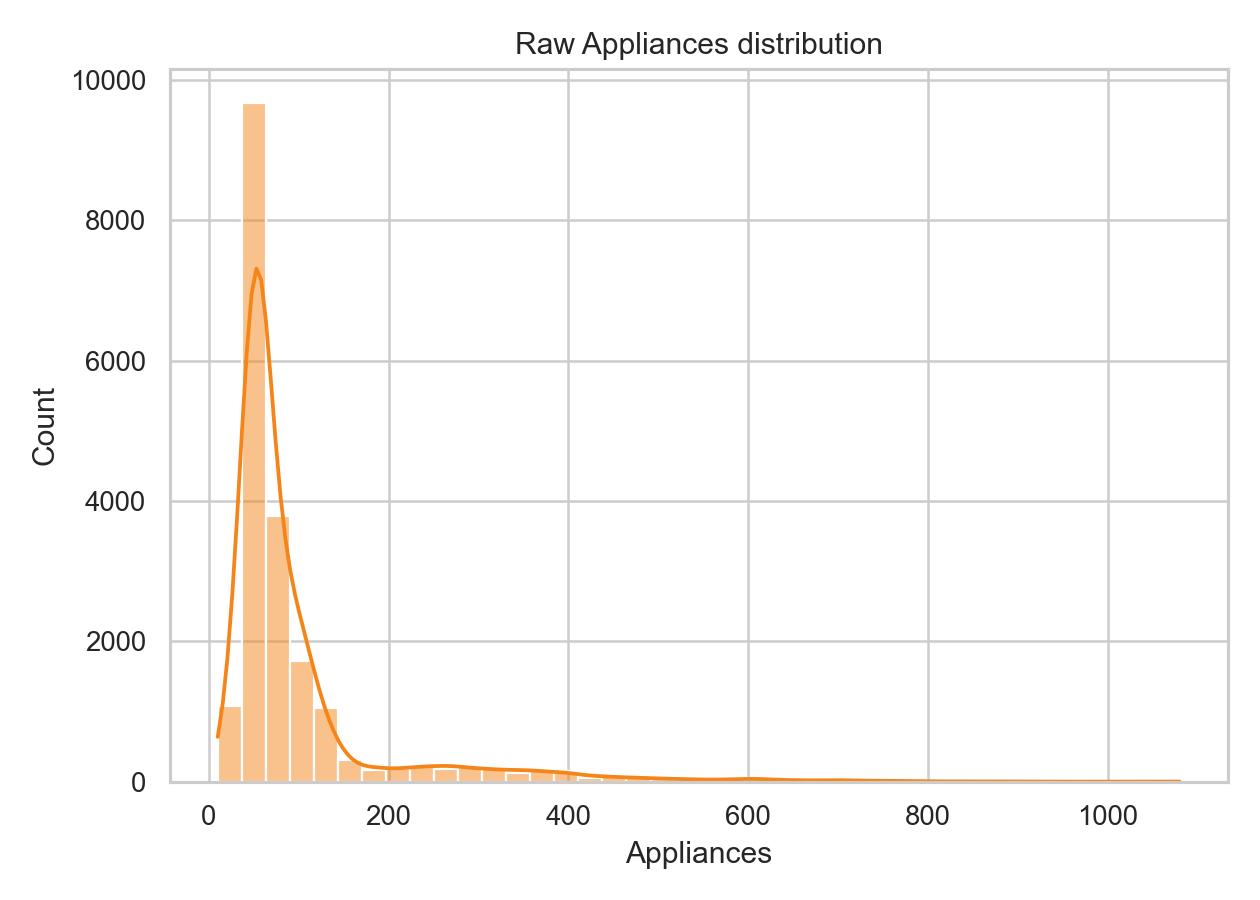
\includegraphics[width=0.78\textwidth]{images/ch1/appliances_energy_distribution_raw.png}
\caption[Minh họa histogram raw Python]{Phân phối gốc (raw) của biến \texttt{Appliances} bằng Python.}
\label{fig:chapter1_histogram_raw}
\end{figure}

\begin{figure}[H]
\centering
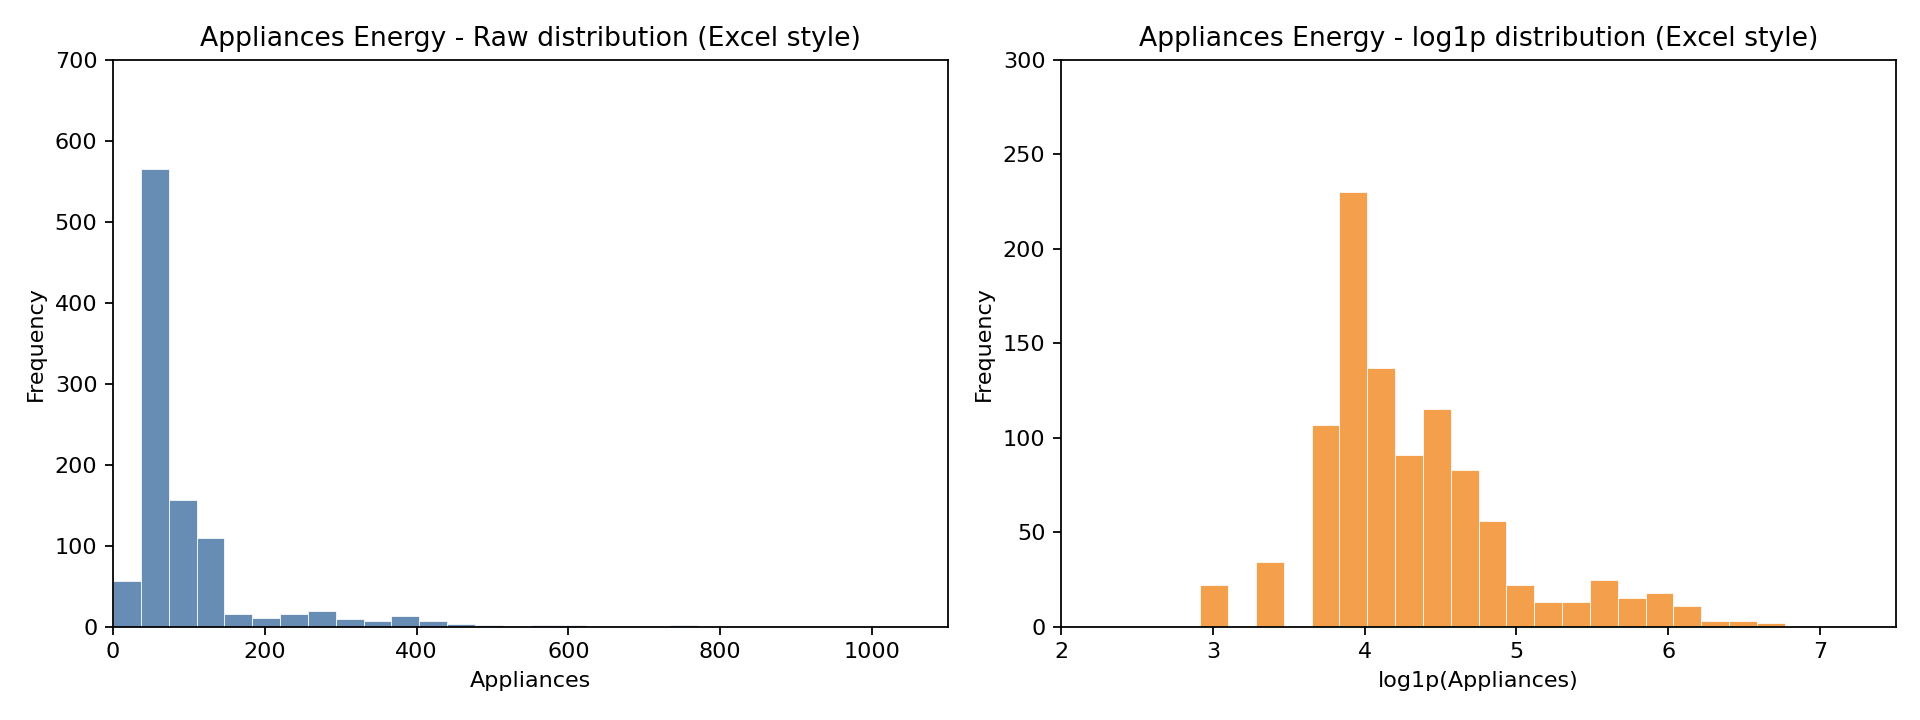
\includegraphics[width=0.78\textwidth]{images/ch1/excel_appliances_raw_vs_log_hist_preview.png}
\caption[Minh họa histogram Excel]{Biểu đồ Histogram của biến \texttt{Appliances} được xây dựng trên Excel. Workbook: \texttt{excel/excel\_visualization\_comparison\_native.xlsx}, sheet \texttt{Appliances Histogram}.}
\label{fig:chapter1_histogram_example_excel}
\end{figure}

\textbf{Nhận xét và lý do chọn.} Histogram được chọn vì \texttt{Appliances} là biến định lượng liên tục và câu hỏi đặt ra là ``giá trị tiêu thụ điện phân bố thế nào?''. Hình~\ref{fig:chapter1_histogram_raw} cho thấy phân phối gốc \textbf{lệch phải mạnh}: phần lớn các khung giờ tiêu thụ ít điện (cột cao ở bên trái), trong khi một số ít khung giờ tiêu thụ rất nhiều (đuôi dài kéo sang phải). So sánh Python (Hình~\ref{fig:chapter1_histogram_raw}) và Excel (Hình~\ref{fig:chapter1_histogram_example_excel}) cho thấy hai công cụ cho ra cùng hình dạng lệch phải, tức là kết luận không phụ thuộc công cụ: dữ liệu này không nên đưa thẳng vào mô hình hồi quy mà cần biến đổi log hoặc xử lý dữ liệu bất thường trước. Python phù hợp khi cần tự động hóa và tái lập; Excel phù hợp khi cần kiểm tra nhanh bằng bảng tính.

\subsubsection{Boxplot (Biểu đồ hộp): phát hiện dữ liệu bất thường dựa trên IQR}

Boxplot hiển thị median, $Q_1$, $Q_3$, IQR và các điểm ngoài ngưỡng $Q_1-1.5\times IQR$ hoặc $Q_3+1.5\times IQR$. Đây là biểu đồ quan trọng để phát hiện dữ liệu bất thường và so sánh phân phối giữa các lớp. Ví dụ boxplot cholesterol theo \texttt{target\_binary} cho phép so sánh mức cholesterol giữa nhóm có và không có bệnh tim. Tác dụng phân tích là phát hiện biến cần xử lý ngoại lệ, đồng thời đánh giá biến định lượng có khả năng phân biệt nhãn hay không. \textbf{Hạn chế:} boxplot không mô tả rõ hình dạng phân phối bên trong; dữ liệu đa đỉnh có thể bị che khuất. Điểm ngoài râu hộp chỉ là ứng viên dữ liệu bất thường, cần kiểm tra thêm bằng kiến thức miền.

\begin{table}[H]
\centering
\caption{Dữ liệu mẫu cho boxplot cholesterol theo nhóm bệnh tim}
\label{tab:chapter1_boxplot_sample_data}
\small
\begin{tabular}{rrrr}
\toprule
Mẫu & \texttt{target\_binary} & \texttt{chol} & Ghi chú \\
\midrule
1 & 0 & 233 & Nhóm không bệnh \\
2 & 0 & 250 & Nhóm không bệnh \\
3 & 1 & 204 & Nhóm có bệnh \\
4 & 1 & 236 & Nhóm có bệnh \\
5 & 0 & 354 & Giá trị cao \\
6 & 1 & 564 & Ứng viên dữ liệu bất thường \\
\bottomrule
\end{tabular}
\end{table}

Bảng \ref{tab:chapter1_boxplot_sample_data} cho thấy dữ liệu boxplot cần một biến định lượng và một biến nhóm. Trước khi vẽ, cần tính các đại lượng hộp: $Q_1$, median, $Q_3$, IQR và biên dữ liệu bất thường.

\begin{table}[H]
\centering
\caption{Tính toán trước khi vẽ boxplot cholesterol}
\label{tab:chapter1_boxplot_calc}
\small
\begin{tabular}{lrr}
\toprule
Thành phần boxplot & Công thức/cách lấy & Kết quả \\
\midrule
$Q_1$ & $P_{25}$ của \texttt{chol} & 211 \\
Median & $P_{50}$ của \texttt{chol} & 241 \\
$Q_3$ & $P_{75}$ của \texttt{chol} & 275 \\
IQR & $Q_3-Q_1$ & 64 \\
Biên dưới & $Q_1-1.5\times IQR$ & 115 \\
Biên trên & $Q_3+1.5\times IQR$ & 371 \\
Ứng viên dữ liệu bất thường & \texttt{chol} $>371$ hoặc $<115$ & 564 \\
\bottomrule
\end{tabular}
\end{table}

Từ các kết quả trên có thể vẽ tay boxplot: hộp kéo từ 211 đến 275, đường giữa ở 241, râu dưới kéo dài đến giá trị nhỏ nhất nằm trong khoảng $1.5 \times IQR$ là 126 (mặc dù biên dưới tính toán lý thuyết là 115 nhưng không có dữ liệu thực tế nào nhỏ hơn 126), râu trên kéo dài đến giá trị lớn nhất nằm trong khoảng $1.5 \times IQR$ là 371, và điểm dữ liệu 564 nằm ngoài râu được biểu diễn riêng biệt là dữ liệu bất thường.

\textbf{Ghi chú về Box plot trong workbook Excel.} Box-and-Whisker là kiểu biểu đồ có trong Excel hiện đại, nhưng workbook minh chứng của báo cáo chỉ lưu các chart object native được script dựng tự động và không nhúng ảnh preview. Vì vậy ví dụ boxplot ở phần này được trình bày bằng Python; sheet \texttt{Heart Boxplot} trong workbook chỉ giữ bảng tóm tắt để người đọc có thể tự dựng lại nếu cần.

\begin{figure}[H]
\centering
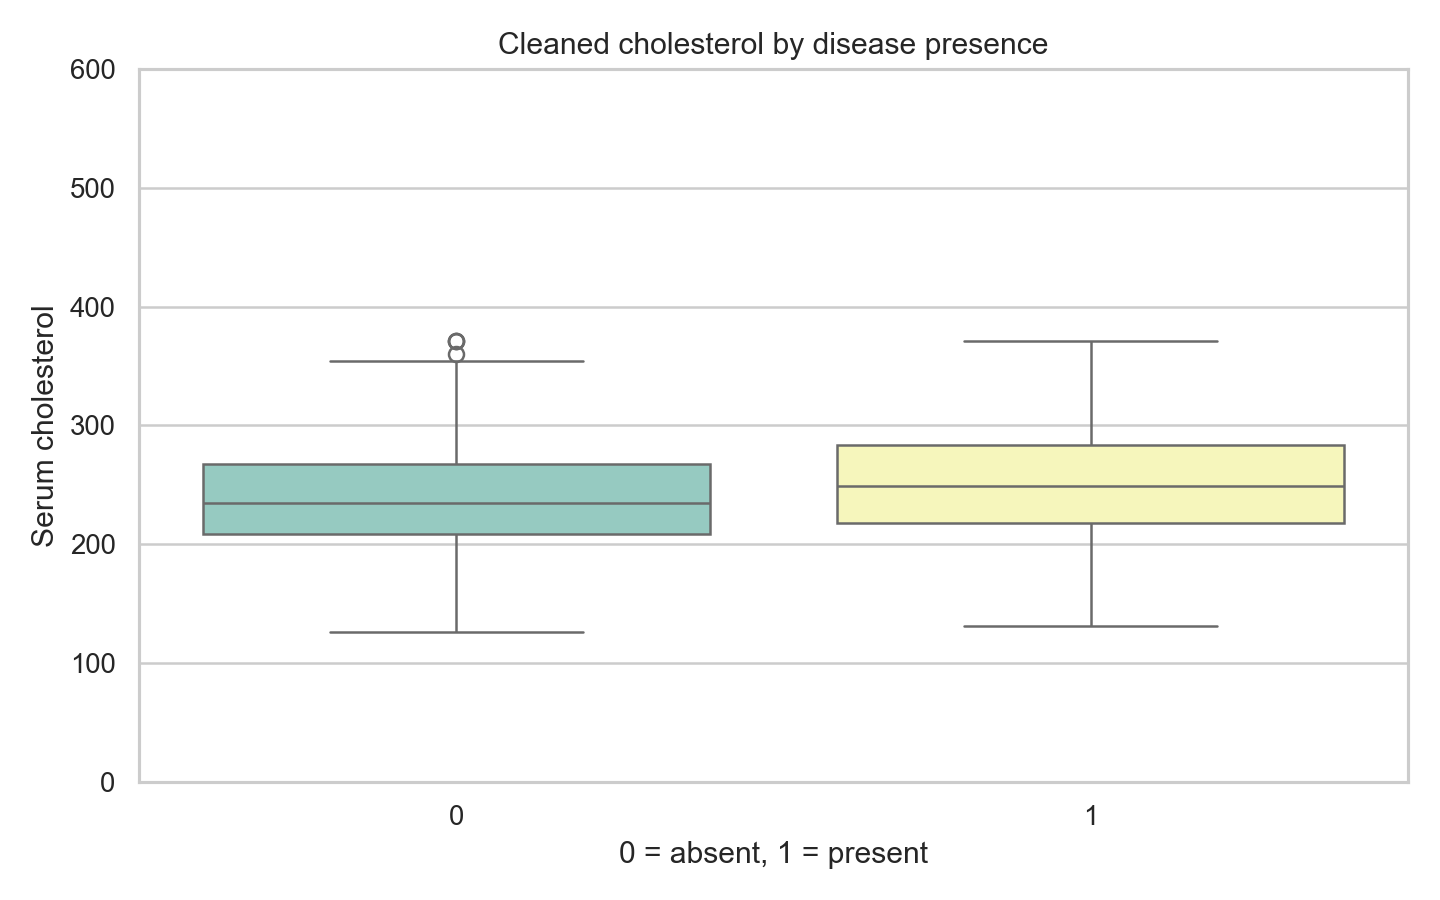
\includegraphics[width=0.90\textwidth]{images/ch1/heart_disease_cholesterol_boxplot.png}
\caption[Minh họa boxplot Heart Disease]{Minh họa boxplot: cholesterol theo nhóm bệnh tim.}
\label{fig:chapter1_boxplot_example}
\end{figure}

\textbf{Nhận xét và lý do chọn.} Boxplot được chọn vì \texttt{chol} là biến định lượng liên tục và câu hỏi phân tích là ``có dữ liệu bất thường hay không, phân phối hai nhóm target khác nhau thế nào?''. Hình \ref{fig:chapter1_boxplot_example} cho thấy cholesterol có các điểm nằm ngoài vùng râu hộp, tức là có ứng viên dữ liệu bất thường theo quy tắc IQR. Median và IQR giúp đọc cấu trúc trung tâm tốt hơn mean khi dữ liệu có giá trị cực trị. So với histogram, boxplot không mô tả chi tiết hình dạng phân phối, nhưng tốt hơn trong việc so sánh hai nhóm và phát hiện điểm bất thường. Vì vậy, mẫu Heart Disease phù hợp với boxplot khi mục tiêu là đánh giá dữ liệu bất thường và khả năng phân biệt nhóm bệnh/không bệnh.

\textbf{Đánh giá.} Kết quả biểu diễn phân phối biến cholesterol theo \texttt{target\_binary} cho thấy sự khác biệt về trung vị và các điểm dữ liệu bất thường. Python phù hợp cho phiên bản báo cáo vì kiểm soát được định dạng, nhãn và tái lập bằng script.

\subsection{Nhóm biểu đồ tương quan và cơ cấu}

Nhóm biểu đồ tương quan và cơ cấu trả lời hai câu hỏi: ``các biến có liên hệ với nhau không?'' và ``các nhóm định tính chiếm tỷ trọng thế nào?''. Scatter plot và heatmap dùng cho biến định lượng; bar chart và pie chart dùng cho biến định tính. Có thể bổ sung pair plot, hexbin plot, stacked bar chart và mosaic plot khi cần phân tích sâu hơn.

\begin{table}[H]
\centering
\caption{Nhóm biểu đồ tương quan và cơ cấu: ý nghĩa, hạn chế và trường hợp áp dụng}
\label{tab:chapter1_relation_structure_chart_group}
\small
\begin{tabular}{p{0.18\textwidth}p{0.25\textwidth}p{0.25\textwidth}p{0.20\textwidth}}
\toprule
Biểu đồ & Ý nghĩa & Trường hợp áp dụng & Hạn chế \\
\midrule
Biểu đồ phân tán (Scatter plot) & Tìm liên hệ tuyến tính/phi tuyến, cụm, điểm bất thường & \texttt{age}--\texttt{thalach}, nhiệt độ--năng lượng & Dễ xảy ra hiện tượng chồng lấp điểm (overplotting) khi kích thước dữ liệu lớn; chỉ phản ánh mối tương quan trực quan bề mặt mà không thể xác lập quan hệ nhân quả trực tiếp. \\
Biểu đồ cột/tròn (Bar/Pie chart) & Xem cơ cấu định tính, lớp phổ biến/hiếm & \texttt{cp}, \texttt{dx}, \texttt{Diagnosis} & Pie khó so sánh nhiều nhóm; bar không thể hiện quan hệ nếu không nhóm/chồng \\
Bản đồ nhiệt tương quan (Correlation heatmap) & Xem tương quan nhiều biến định lượng & Chọn đặc trưng Heart Disease, Breast Cancer & Chủ yếu phản ánh mối liên hệ tương quan tuyến tính đơn biến (Pearson); không thể hiện được các mối quan hệ phi tuyến phức tạp và không khẳng định quan hệ nhân quả. \\
Biểu đồ cặp/tổ ong (Pair/Hexbin plot) & Xem nhiều cặp biến hoặc mật độ điểm dày & EDA nhiều biến định lượng & Dễ rối, tốn không gian báo cáo \\
Biểu đồ cột chồng/mảnh ghép (Stacked bar/Mosaic) & Xem quan hệ hai biến định tính & \texttt{dx} theo \texttt{localization}, target theo giới tính & Khó đọc khi nhiều nhóm nhỏ \\
\bottomrule
\end{tabular}
\end{table}

\subsubsection{Scatter plot (Biểu đồ phân tán): tìm liên hệ tuyến tính/phi tuyến}

Scatter plot biểu diễn mối quan hệ giữa hai biến định lượng. Nếu các điểm tạo thành xu hướng tăng/giảm, có thể tồn tại liên hệ tuyến tính hoặc phi tuyến. Trong Heart Disease, scatter plot giữa \texttt{age} và \texttt{thalach} giúp kiểm tra xu hướng tuổi cao đi kèm nhịp tim tối đa thấp hơn hay không. Tác dụng phân tích là phát hiện quan hệ biến, cụm quan sát và điểm bất thường theo cặp biến. \textbf{Hạn chế:} khi số điểm quá lớn, điểm bị chồng lên nhau làm khó đọc; xu hướng quan sát được không khẳng định quan hệ nhân quả.

\begin{table}[H]
\centering
\caption{Dữ liệu mẫu cho scatter plot tuổi và nhịp tim tối đa}
\label{tab:chapter1_scatter_sample_data}
\small
\begin{tabular}{rrrr}
\toprule
Mẫu & \texttt{age} & \texttt{thalach} & \texttt{target\_binary} \\
\midrule
1 & 63 & 150 & 0 \\
2 & 67 & 108 & 1 \\
3 & 37 & 187 & 0 \\
4 & 41 & 172 & 0 \\
5 & 56 & 178 & 1 \\
6 & 62 & 160 & 1 \\
\bottomrule
\end{tabular}
\end{table}

Bảng \ref{tab:chapter1_scatter_sample_data} minh họa mỗi dòng là một điểm trên scatter plot. Trước khi vẽ, cần chuyển mỗi dòng thành tọa độ $(x,y)$, với $x=\texttt{age}$ và $y=\texttt{thalach}$; nếu tô màu thì dùng thêm \texttt{target\_binary}.

\begin{table}[H]
\centering
\caption{Tính tọa độ trước khi vẽ scatter plot}
\label{tab:chapter1_scatter_calc}
\small
\begin{tabular}{rrrr}
\toprule
Mẫu & Tọa độ $(x,y)$ & Nhóm màu & Diễn giải \\
\midrule
1 & $(63,150)$ & 0 & Tuổi 63, nhịp tim tối đa 150 \\
2 & $(67,108)$ & 1 & Tuổi 67, nhịp tim tối đa 108 \\
3 & $(37,187)$ & 0 & Tuổi 37, nhịp tim tối đa 187 \\
4 & $(41,172)$ & 0 & Tuổi 41, nhịp tim tối đa 172 \\
5 & $(56,178)$ & 1 & Tuổi 56, nhịp tim tối đa 178 \\
6 & $(62,160)$ & 1 & Tuổi 62, nhịp tim tối đa 160 \\
\bottomrule
\end{tabular}
\end{table}

Từ bảng tọa độ này có thể vẽ tay scatter plot bằng cách đặt từng điểm lên hệ trục; nhóm màu 0/1 giúp phân biệt bệnh/không bệnh.

\textbf{Các bước thao tác vẽ scatter plot bằng Excel.} Để bảo đảm tính tái lập, báo cáo trình bày thao tác cụ thể trên Microsoft Excel cho biểu đồ đại diện ở Bảng \ref{tab:chapter1_scatter_calc} (scatter plot giữa \texttt{age} và \texttt{thalach}, tô màu theo \texttt{target\_binary}):
\begin{enumerate}[leftmargin=2.2em,label=\textbf{Bước \arabic*.}]
 \item \textbf{Chuẩn bị dữ liệu:} mở file \texttt{outputs/cleaned/heart\_disease\_cleaned.csv} trong Excel; đảm bảo ba cột \texttt{age}, \texttt{thalach}, \texttt{target\_binary} nằm cạnh nhau và có hàng tiêu đề (ví dụ để \texttt{age} ở cột A, \texttt{thalach} ở cột B, \texttt{target\_binary} ở cột C).
 \item \textbf{Bôi đen vùng dữ liệu:} quét chọn vùng chứa hai cột \texttt{age} (trục $x$) và \texttt{thalach} (trục $y$), bao gồm cả hàng tiêu đề, ví dụ \texttt{A1:B304}.
 \item \textbf{Chèn biểu đồ:} vào tab \textbf{Insert} $\rightarrow$ nhóm \textbf{Charts} $\rightarrow$ chọn \textbf{Scatter} (biểu tượng điểm chấm) $\rightarrow$ chọn \textbf{Scatter with only Markers}. Excel tự động vẽ các điểm lên hệ trục.
 \item \textbf{Tô màu theo nhóm:} vì một scatter plot mặc định chỉ có một màu, để phân biệt bệnh/không bệnh cần tách dữ liệu thành hai chuỗi (series): chèn thêm cột \texttt{thalach\_0} và \texttt{thalach\_1} dùng hàm \texttt{=IF(C2=0,B2,NA())} và \texttt{=IF(C2=1,B2,NA())}; sau đó chọn \textbf{Select Data} trên biểu đồ $\rightarrow$ \textbf{Add} từng chuỗi với $x$ là cột \texttt{age}, $y$ lần lượt là \texttt{thalach\_0} và \texttt{thalach\_1}; đặt màu khác nhau cho hai chuỗi (ví dụ xanh cho \texttt{target\_binary}=0, đỏ cho \texttt{target\_binary}=1).
 \item \textbf{Định dạng trục và nhãn:} nhấp vào biểu đồ $\rightarrow$ tab \textbf{Chart Design} $\rightarrow$ \textbf{Add Chart Element} $\rightarrow$ đặt \textbf{Axis Titles} là ``Tuổi (age)'' cho trục $x$ và ``Nhịp tim tối đa (thalach)'' cho trục $y$; thêm \textbf{Chart Title} và \textbf{Legend} để ghi rõ ý nghĩa hai màu.
 \item \textbf{(Tuỳ chọn) Đường xu hướng:} để thấy quan hệ âm, nhấp chuột phải vào một chuỗi $\rightarrow$ \textbf{Add Trendline} $\rightarrow$ chọn \textbf{Linear} và tick \textbf{Display Equation on chart}; hệ số góc âm sẽ xác nhận xu hướng ``tuổi tăng, nhịp tim tối đa giảm''.
 \item \textbf{Xuất ảnh:} nhấp chuột phải vào vùng biểu đồ $\rightarrow$ \textbf{Save as Picture} $\rightarrow$ chọn định dạng PNG để đưa vào báo cáo.
\end{enumerate}
Quy trình bảy bước trên áp dụng chung cho mọi scatter plot trong báo cáo; với các biến khác (ví dụ \texttt{T1}--\texttt{Appliances} trong Appliances Energy) chỉ cần thay vùng dữ liệu ở Bước 2. Kết quả thu được ở Hình \ref{fig:chapter1_scatter_example_excel} cho hình dạng xu hướng tương tự phiên bản Python ở Hình \ref{fig:chapter1_scatter_example}, chứng tỏ thao tác Excel và script Python cho ra cùng một kết luận phân tích.

\begin{figure}[H]
\centering
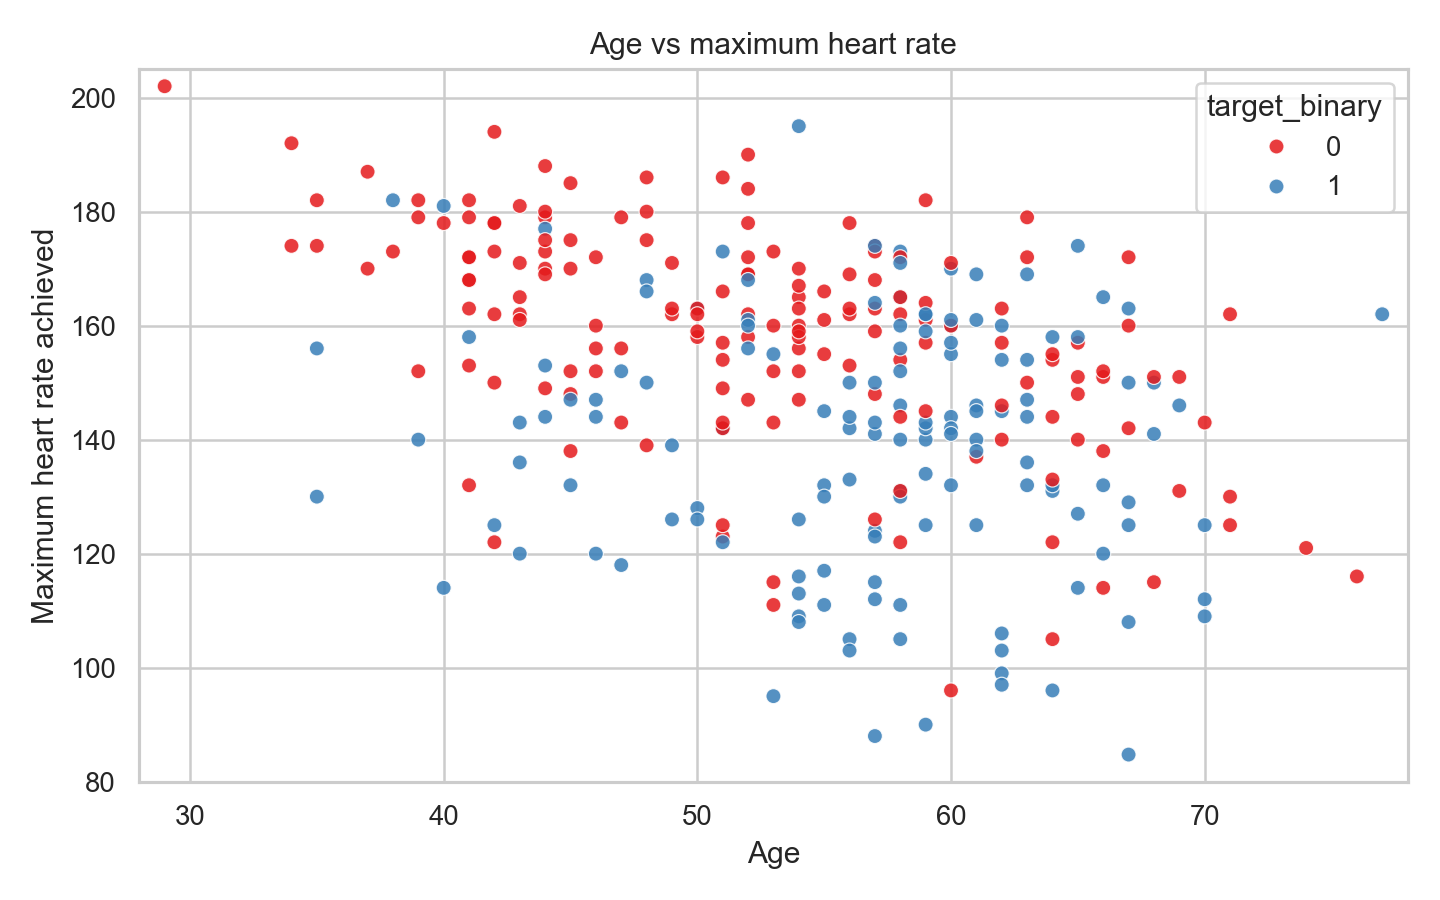
\includegraphics[width=0.90\textwidth]{images/ch1/heart_disease_age_thalach_scatter.png}
\caption[Minh họa scatter plot Python]{Minh họa scatter plot tuổi và nhịp tim tối đa trong Heart Disease bằng Python.}
\label{fig:chapter1_scatter_example}
\end{figure}

\begin{figure}[H]
\centering
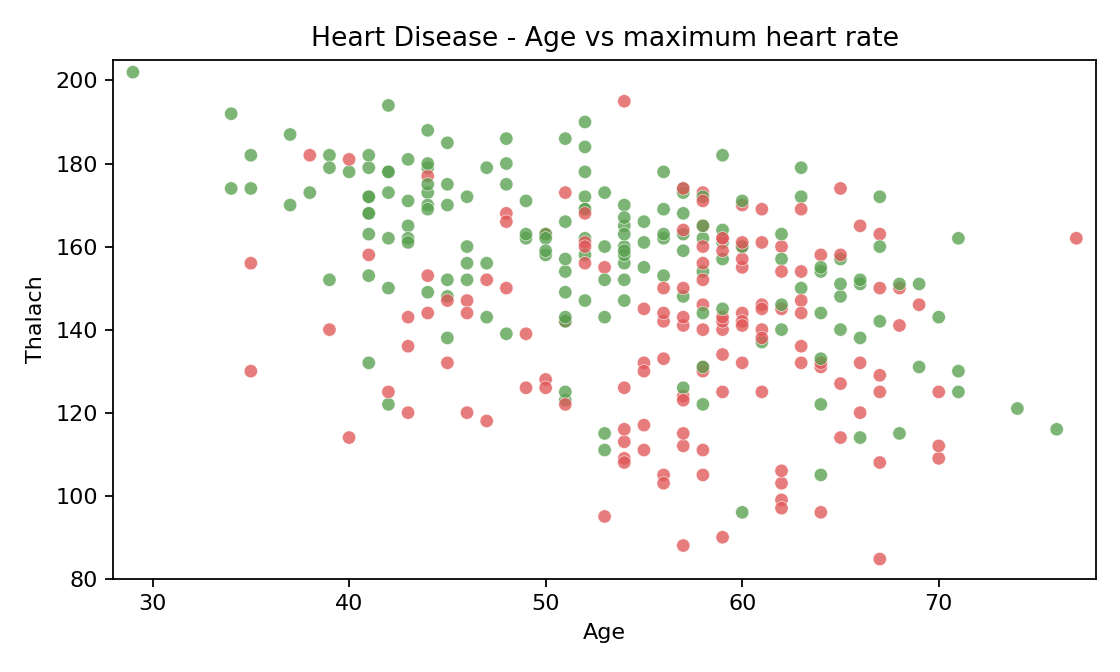
\includegraphics[width=0.90\textwidth]{images/ch1/excel_heart_age_thalach_scatter_preview.png}
\caption[Minh họa scatter plot Excel]{Minh họa scatter plot tuổi và nhịp tim tối đa trong Heart Disease bằng Excel. Workbook: \texttt{excel/excel\_visualization\_comparison\_native.xlsx}, sheet \texttt{Heart Scatter}.}
\label{fig:chapter1_scatter_example_excel}
\end{figure}

\textbf{Nhận xét và lý do chọn.} Scatter plot được chọn vì \texttt{age} và \texttt{thalach} đều là biến định lượng, mục tiêu là kiểm tra quan hệ giữa hai biến thay vì chỉ xem từng biến riêng lẻ. Hình \ref{fig:chapter1_scatter_example} cho thấy xu hướng âm: tuổi tăng thì nhịp tim tối đa có xu hướng giảm. So với histogram và boxplot, scatter plot biểu diễn từng cặp quan sát nên phù hợp để phát hiện quan hệ tuyến tính, phi tuyến, cụm điểm hoặc điểm bất thường theo cặp biến. Python và Excel cho hình dạng xu hướng tương tự; Python thuận tiện khi cần tô màu theo target hoặc tính correlation, còn Excel giúp kiểm tra nhanh bằng thao tác trực quan.

\subsubsection{Bar chart/Pie chart (Biểu đồ cột/tròn): cơ cấu định tính}

Bar chart và pie chart dùng cho biến định tính. Bar chart để so sánh tần suất giữa các nhóm; pie chart để mô tả tỷ trọng khi số nhóm ít và tỷ lệ cần trình bày nhanh. Trong báo cáo, bar chart được ưu tiên hơn pie chart vì dễ so sánh hơn, đặc biệt với các biến có nhiều lớp như \texttt{localization} trong HAM10000. Tác dụng phân tích là nhận diện mất cân bằng lớp, lớp hiếm và cơ cấu dữ liệu đầu vào. \textbf{Hạn chế:} pie chart khó so sánh khi có nhiều nhóm hoặc tỷ lệ gần nhau; bar chart chỉ mô tả cơ cấu một biến nếu không mở rộng thành grouped/stacked bar.

\begin{table}[H]
\centering
\caption{Dữ liệu mẫu cho bar chart loại đau ngực}
\label{tab:chapter1_bar_sample_data}
\small
\begin{tabular}{lrr}
\toprule
Loại đau ngực \texttt{cp} & Tần suất & Tỷ lệ xấp xỉ \\
\midrule
1 & 23 & 7.6\% \\
2 & 50 & 16.5\% \\
3 & 86 & 28.4\% \\
4 & 144 & 47.5\% \\
\bottomrule
\end{tabular}
\end{table}

Bảng \ref{tab:chapter1_bar_sample_data} là dữ liệu đã tổng hợp theo nhóm. Trước khi vẽ bar chart hoặc pie chart, cần tính tần suất và tỷ lệ: $p_j=f_j/n$ với $n=303$.

\begin{table}[H]
\centering
\caption{Tính toán trước khi vẽ bar chart/pie chart biến \texttt{cp}}
\label{tab:chapter1_bar_calc}
\small
\begin{tabular}{lrrr}
\toprule
Giá trị \texttt{cp} & $f_j$ & $p_j=f_j/303$ & Góc pie chart \\
\midrule
1 & 23 & 7.6\% & 27.3$^\circ$ \\
2 & 50 & 16.5\% & 59.4$^\circ$ \\
3 & 86 & 28.4\% & 102.2$^\circ$ \\
4 & 144 & 47.5\% & 171.1$^\circ$ \\
\bottomrule
\end{tabular}
\end{table}

Từ bảng này có thể vẽ tay bar chart bằng chiều cao cột $f_j$; nếu vẽ pie chart thì dùng góc $p_j\times360^\circ$ cho từng lát cắt.

\begin{figure}[H]
\centering
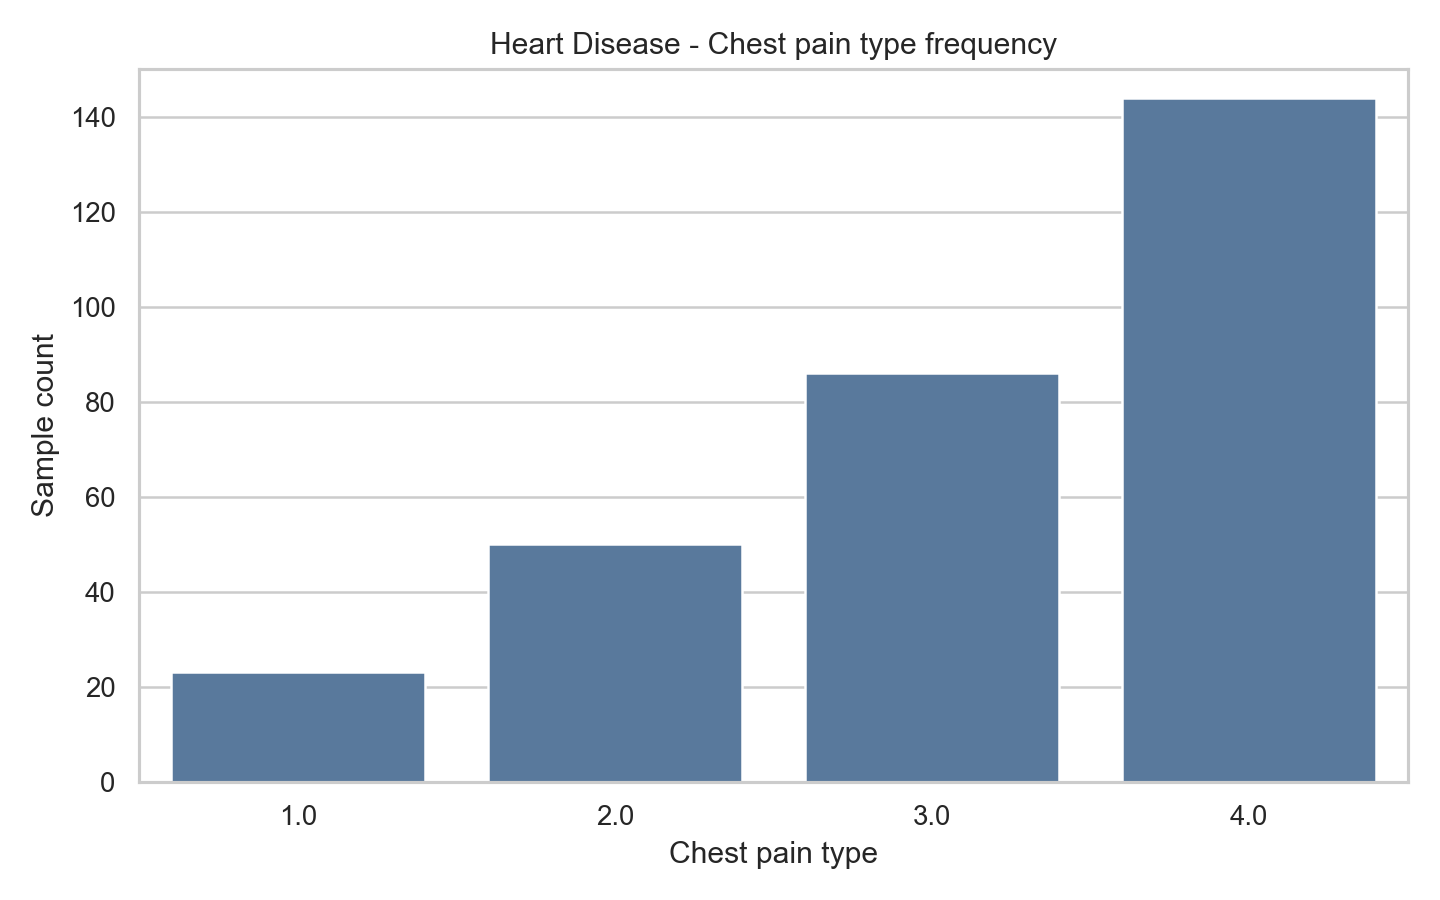
\includegraphics[width=0.90\textwidth]{images/ch1/heart_disease_chest_pain_bar.png}
\caption[Minh họa bar chart Python]{Minh họa bar chart tần suất loại đau ngực Heart Disease bằng Python.}
\label{fig:chapter1_bar_example}
\end{figure}

\begin{figure}[H]
\centering
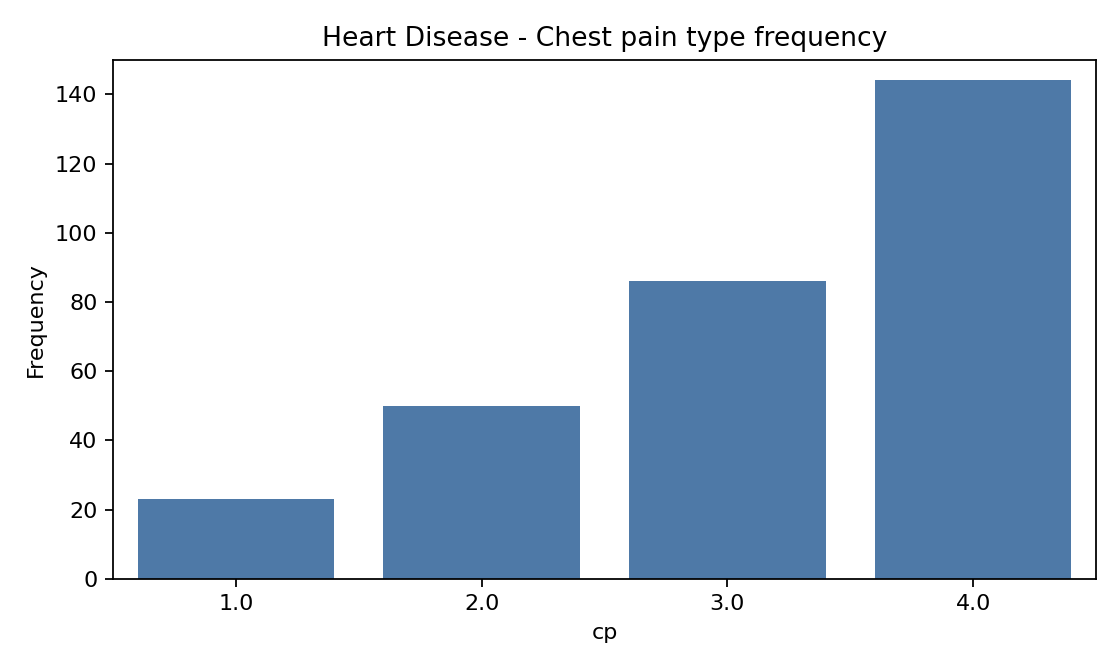
\includegraphics[width=0.90\textwidth]{images/ch1/excel_heart_cp_bar_preview.png}
\caption[Minh họa bar chart Excel]{Minh họa bar chart tần suất loại đau ngực Heart Disease bằng Excel. Workbook: \texttt{excel/excel\_visualization\_comparison\_native.xlsx}, sheet \texttt{Heart Frequency}.}
\label{fig:chapter1_bar_example_excel}
\end{figure}

\textbf{Nhận xét và lý do chọn.} Bar chart được chọn vì \texttt{cp} là biến định tính/rời rạc, biểu diễn loại đau ngực. Với biến loại nhóm, histogram không phù hợp vì các mã 1--4 không phải thang đo liên tục; scatter plot cũng không có ý nghĩa nếu chỉ phân tích một biến định tính. Hình \ref{fig:chapter1_bar_example} cho thấy \texttt{cp=4} chiếm nhiều nhất, tức cơ cấu loại đau ngực không cân bằng. Bar chart tốt hơn pie chart trong mẫu này vì người đọc dễ so sánh chiều cao cột giữa bốn nhóm. Python và Excel cho cùng thứ tự nhóm, chứng minh bảng tần suất được tính nhất quán giữa hai công cụ.

\textbf{Trực quan hóa dữ liệu bằng biểu đồ tròn (Pie Chart): So sánh dạng 2D và 3D.} Trong trực quan hóa dữ liệu khoa học, biểu đồ tròn dạng 2D được coi là chuẩn mực trình bày, trong khi biểu đồ tròn 3D ít được khuyến nghị sử dụng. Bản chất góc nghiêng phối cảnh và chiều sâu của không gian 3D làm sai lệch tỷ lệ thị giác của người xem: các phân phần nằm ở phía trước (gần mắt nhìn hơn) trông sẽ lớn hơn thực tế, ngược lại các phần ở phía sau bị thu nhỏ lại dù có cùng tỷ trọng. Điều này dễ dẫn đến việc ước lượng sai lệch cấu trúc dữ liệu.

Hơn nữa, việc sử dụng hiệu ứng tách mảnh (exploded pie chart) trong không gian 3D càng làm gia tăng độ méo hình học, do chiều cao của miếng bánh tạo ra thể tích ảo không tỷ lệ thuận với giá trị thực tế của dữ liệu. Biểu đồ tròn 2D duy trì chính xác tỷ lệ góc ở tâm $\theta_i = p_i \times 360^\circ$ (như tính toán ở bảng thống kê cơ cấu lớp), giúp truyền tải cấu trúc thuộc tính định tính một cách trung thực nhất. Do đó, toàn bộ biểu đồ cột và biểu đồ tròn trong nghiên cứu này đều được thống nhất biểu diễn dưới dạng 2D phẳng để đảm bảo tính khách quan và chuẩn mực khoa học.

\subsection{Các dạng biểu đồ khác}

Nhóm này dùng cho các trường hợp ngoài phân phối một biến, tương quan hai biến hoặc cơ cấu định tính đơn giản. Các dạng quan trọng gồm line chart cho chuỗi thời gian, rolling mean/area chart để làm mượt hoặc nhấn mạnh xu hướng, confusion matrix để đánh giá phân loại, prediction vs actual để đánh giá hồi quy/dự báo, image grid để kiểm tra dữ liệu ảnh.

\begin{table}[H]
\centering
\caption{Các dạng biểu đồ khác: ý nghĩa, hạn chế và trường hợp áp dụng}
\label{tab:chapter1_other_chart_group}
\small
\begin{tabular}{p{0.18\textwidth}p{0.25\textwidth}p{0.25\textwidth}p{0.20\textwidth}}
\toprule
Biểu đồ & Ý nghĩa & Trường hợp áp dụng & Hạn chế \\
\midrule
Line chart & Trend, seasonality, biến động theo thời gian & Appliances Energy, HAR, MHEALTH & Dễ nhiễu nếu dữ liệu dao động mạnh \\
Rolling mean/Area chart & Làm mượt hoặc nhấn mạnh tổng lượng & Tiêu thụ điện theo ngày/tuần & Che mất biến động ngắn hạn \\
Confusion matrix & Lỗi phân loại theo lớp & Heart Disease, HAM10000, Breast Cancer & Cần mô hình đã huấn luyện; phụ thuộc ngưỡng \\
Prediction vs Actual & So sánh dự báo và thực tế & Regression/dự báo Appliances & Không chỉ rõ nguyên nhân sai số \\
Image grid/montage & Kiểm tra chất lượng ảnh, lỗi nhãn & HAM10000 & Chủ quan, chỉ xem được mẫu nhỏ \\
\bottomrule
\end{tabular}
\end{table}

\subsubsection{Line chart (Biểu đồ đường) cho chuỗi thời gian}

Line chart đặt thời gian trên trục hoành và giá trị quan sát trên trục tung. Biểu đồ này bắt buộc với nhóm B để phân tích trend, seasonality, biến động bất thường và thời điểm thay đổi. Với Appliances Energy, dữ liệu có 19,735 mẫu từ 2016-01-11 17:00:00 đến 2016-05-27 18:00:00, tần suất phổ biến 10 phút/mẫu. Do đó line chart theo ngày được dùng để làm mượt xu hướng tiêu thụ năng lượng. Tác dụng phân tích là chọn cách chia train/test theo thời gian và đánh giá biến động trước khi dự báo. \textbf{Hạn chế:} line chart dễ bị nhiễu nếu tần suất lấy mẫu dày và biến động mạnh; cần sắp xếp thời gian đúng, xử lý missing timestamp và cân nhắc rolling mean.

\begin{table}[H]
\centering
\caption{Dữ liệu mẫu cho line chart Appliances Energy theo thời gian}
\label{tab:chapter1_line_sample_data}
\small
\begin{tabular}{lr}
\toprule
Thời điểm & \texttt{Appliances} \\
\midrule
2016-01-11 17:00 & 60 \\
2016-01-11 17:10 & 60 \\
2016-01-11 17:20 & 50 \\
2016-01-11 17:30 & 50 \\
2016-01-11 17:40 & 60 \\
2016-01-11 17:50 & 50 \\
\bottomrule
\end{tabular}
\end{table}

Bảng \ref{tab:chapter1_line_sample_data} cho thấy điều kiện cần của line chart là có biến thời gian được sắp xếp. Trước khi vẽ, cần chuyển từng dòng thành điểm $(t,y)$, với $t$ là thời điểm và $y=\texttt{Appliances}$; nếu vẽ đường trung bình trượt thì tính thêm rolling mean.

\begin{table}[H]
\centering
\caption{Tính tọa độ và rolling mean trước khi vẽ line chart}
\label{tab:chapter1_line_calc}
\small
\begin{tabular}{lrr}
\toprule
Thời điểm & $y_t$ & Rolling mean 3 mẫu \\
\midrule
2016-01-11 17:00 & 60 & -- \\
2016-01-11 17:10 & 60 & -- \\
2016-01-11 17:20 & 50 & 56.67 \\
2016-01-11 17:30 & 50 & 53.33 \\
2016-01-11 17:40 & 60 & 53.33 \\
2016-01-11 17:50 & 50 & 53.33 \\
\bottomrule
\end{tabular}
\end{table}

Công thức rolling mean 3 mẫu là $\bar{y}_{t,3}=(y_t+y_{t-1}+y_{t-2})/3$, ví dụ tại 17:20: $(60+60+50)/3=56.67$. Từ bảng này có thể vẽ tay line chart bằng cách nối các điểm theo thứ tự thời gian.

\begin{figure}[H]
\centering
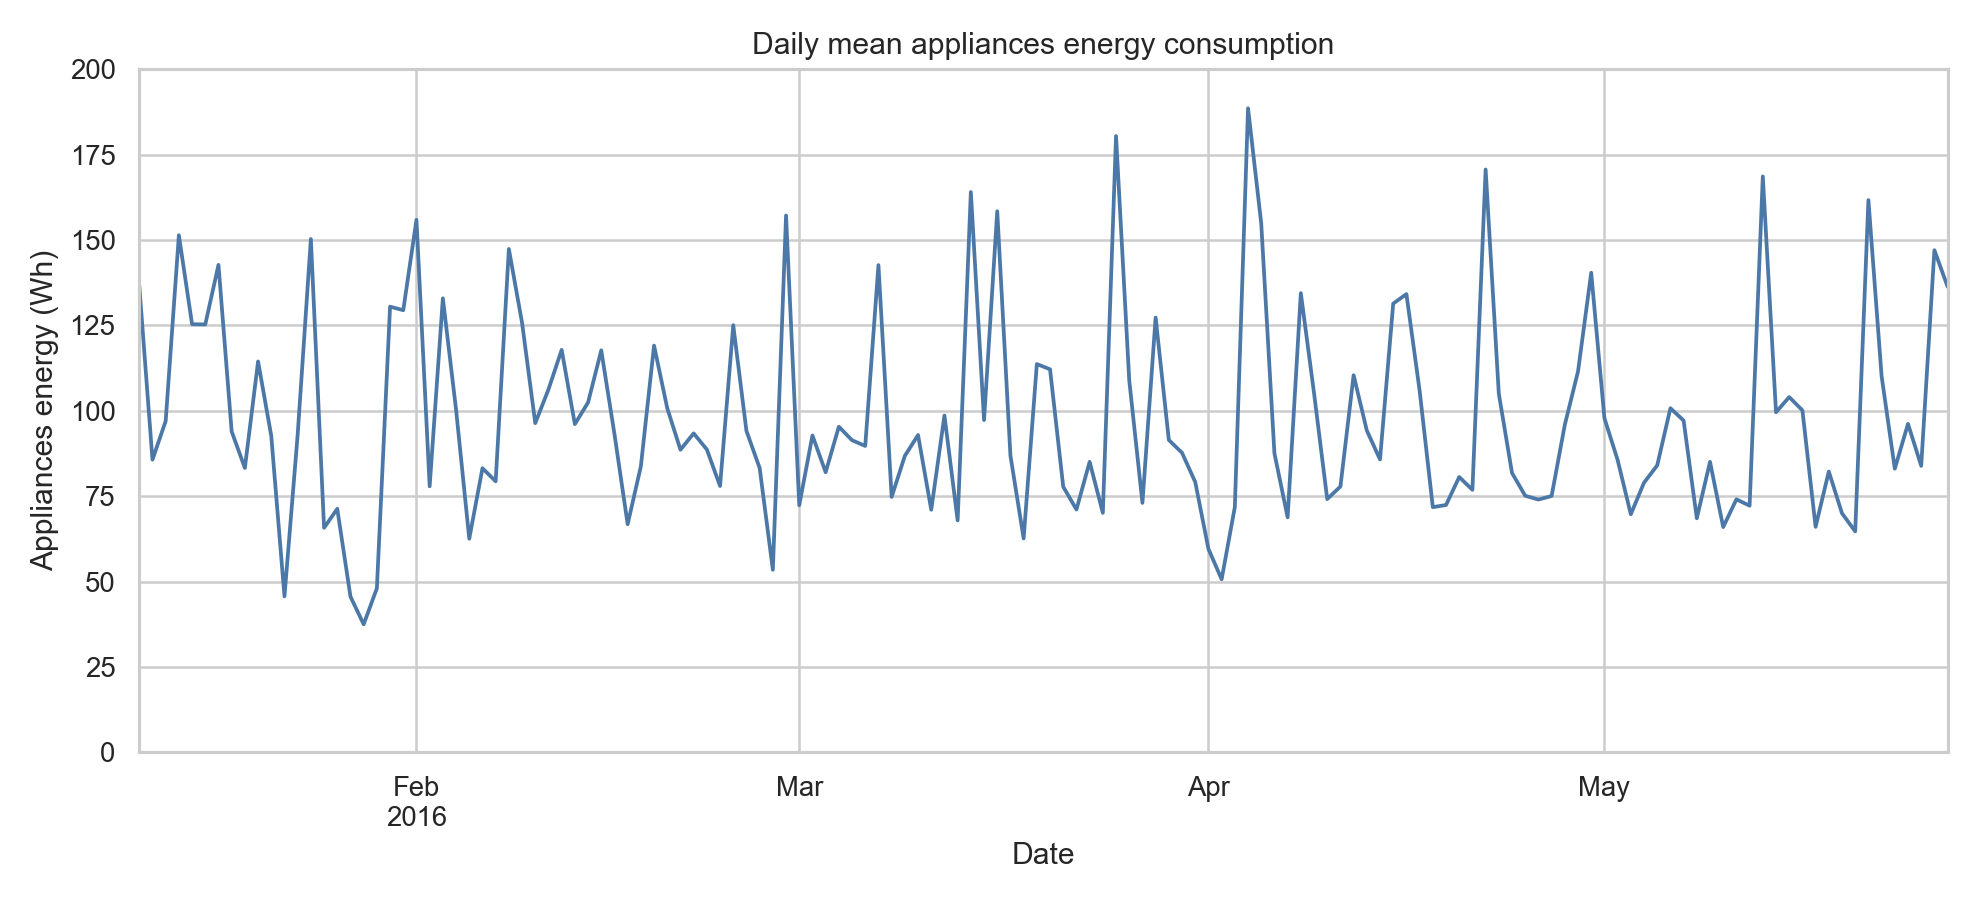
\includegraphics[width=0.90\textwidth]{images/ch1/appliances_energy_daily_line.png}
\caption[Minh họa line chart Python]{Minh họa line chart tiêu thụ năng lượng theo ngày trong Appliances Energy bằng Python.}
\label{fig:chapter1_line_example}
\end{figure}

\begin{figure}[H]
\centering
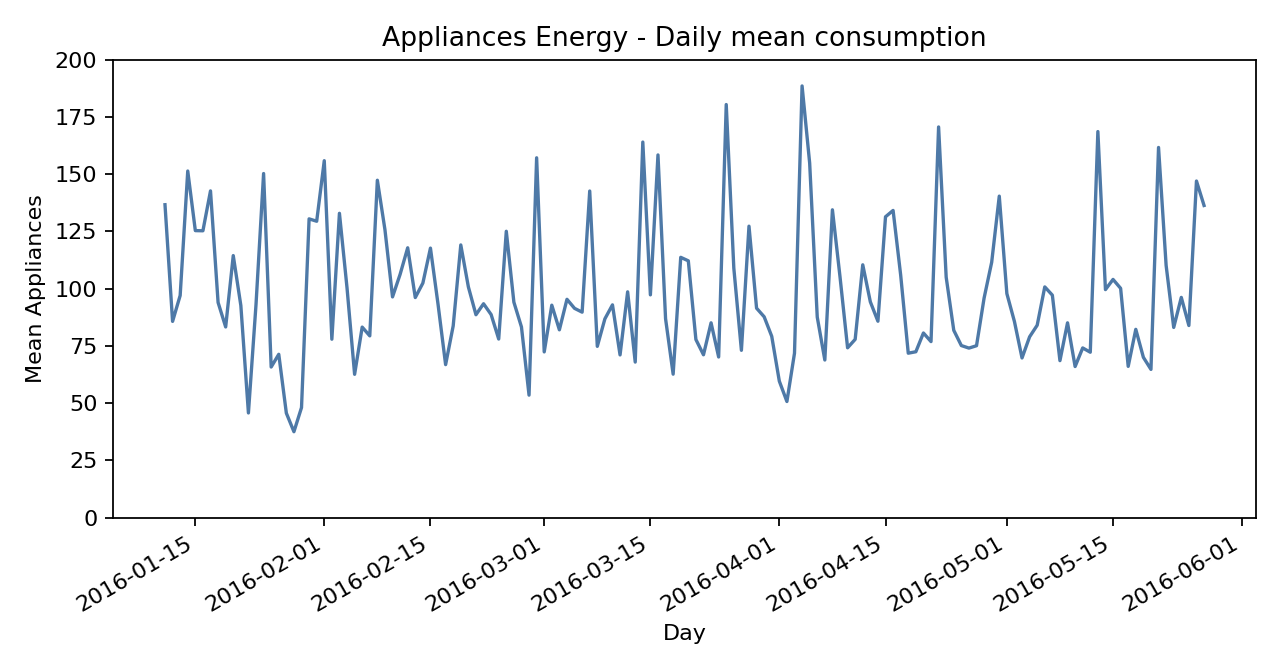
\includegraphics[width=0.90\textwidth]{images/ch1/excel_appliances_daily_line_preview.png}
\caption[Minh họa line chart Excel]{Minh họa line chart tiêu thụ năng lượng theo ngày trong Appliances Energy bằng Excel. Workbook: \texttt{excel/excel\_visualization\_comparison\_native.xlsx}, sheet \texttt{Appliances Daily}.}
\label{fig:chapter1_line_example_excel}
\end{figure}

\textbf{Nhận xét và lý do chọn.} Line chart được chọn vì Appliances Energy có trục thời gian rõ ràng, mỗi quan sát gắn với thời điểm thu thập. Nếu dùng histogram, ta chỉ biết phân phối mức tiêu thụ nhưng mất thông tin thứ tự thời gian; nếu dùng bar chart, xu hướng theo ngày không rõ. Hình \ref{fig:chapter1_line_example} cho thấy mức tiêu thụ dao động theo ngày, có các giai đoạn tăng/giảm và các điểm cao bất thường. So sánh Python và Excel cho thấy xu hướng tổng thể thống nhất. Vì vậy, line chart là lựa chọn phù hợp nhất để phân tích trend, seasonality và làm cơ sở cho quyết định chia train/test theo thời gian ở bài toán dự báo.

\subsubsection{Correlation heatmap (Bản đồ nhiệt tương quan): tương quan nhiều biến định lượng}

Correlation heatmap biểu diễn ma trận tương quan giữa các biến định lượng. Màu sắc giúp nhận diện nhanh cặp biến có tương quan dương hoặc âm. Biểu đồ này hữu ích trong bước lựa chọn đặc trưng và phát hiện đa cộng tuyến trước khi huấn luyện mô hình.

Hệ số tương quan Pearson giữa hai biến $X$ và $Y$ được tính bằng:

\begin{equation}
r_{XY} = \frac{\sum_{i=1}^{n}(x_i-\bar{x})(y_i-\bar{y})}{\sqrt{\sum_{i=1}^{n}(x_i-\bar{x})^2}\sqrt{\sum_{i=1}^{n}(y_i-\bar{y})^2}}
\end{equation}

Giá trị $r_{XY}$ nằm trong khoảng $[-1, 1]$. Giá trị gần 1 biểu thị tương quan dương mạnh; gần -1 biểu thị tương quan âm mạnh; gần 0 biểu thị mối quan hệ tuyến tính yếu. Tuy nhiên, tương quan không đồng nghĩa với quan hệ nhân quả, nên heatmap chỉ nên được xem là công cụ thăm dò ban đầu.

\begin{table}[H]
\centering
\caption{Dữ liệu mẫu cho correlation heatmap Heart Disease}
\label{tab:chapter1_heatmap_sample_data}
\small
\begin{tabular}{rrrrr}
\toprule
Mẫu & \texttt{age} & \texttt{trestbps} & \texttt{chol} & \texttt{thalach} \\
\midrule
1 & 63 & 145 & 233 & 150 \\
2 & 67 & 160 & 286 & 108 \\
3 & 37 & 130 & 250 & 187 \\
4 & 41 & 130 & 204 & 172 \\
5 & 56 & 120 & 236 & 178 \\
6 & 62 & 140 & 268 & 160 \\
\bottomrule
\end{tabular}
\end{table}

Bảng \ref{tab:chapter1_heatmap_sample_data} gồm nhiều biến định lượng trên cùng các mẫu. Từ bảng này, hệ số tương quan được tính cho từng cặp biến, sau đó đưa vào ma trận màu của heatmap. Để chứng minh heatmap không phải hình vẽ ngẫu nhiên, Bảng \ref{tab:chapter1_heatmap_calc} đưa ra một số hệ số tương quan đã tính trước khi tô màu.

\begin{table}[H]
\centering
\caption{Tính toán tương quan trước khi vẽ heatmap}
\label{tab:chapter1_heatmap_calc}
\small
\begin{tabular}{lrr}
\toprule
Cặp biến & Hệ số $r$ & Ý nghĩa màu \\
\midrule
\texttt{age} -- \texttt{thalach} & -0.39 & Tương quan âm, màu lạnh \\
\texttt{age} -- \texttt{trestbps} & 0.28 & Tương quan dương yếu, màu ấm nhạt \\
\texttt{chol} -- \texttt{trestbps} & 0.13 & Gần trung tính \\
\texttt{chol} -- \texttt{thalach} & -0.01 & Gần 0, màu trung tính \\
\bottomrule
\end{tabular}
\end{table}

Từ các hệ số này có thể vẽ tay heatmap bằng cách lập ma trận biến--biến, ghi $r$ vào từng ô và gán màu theo độ lớn/dấu của $r$.

\begin{figure}[H]
\centering
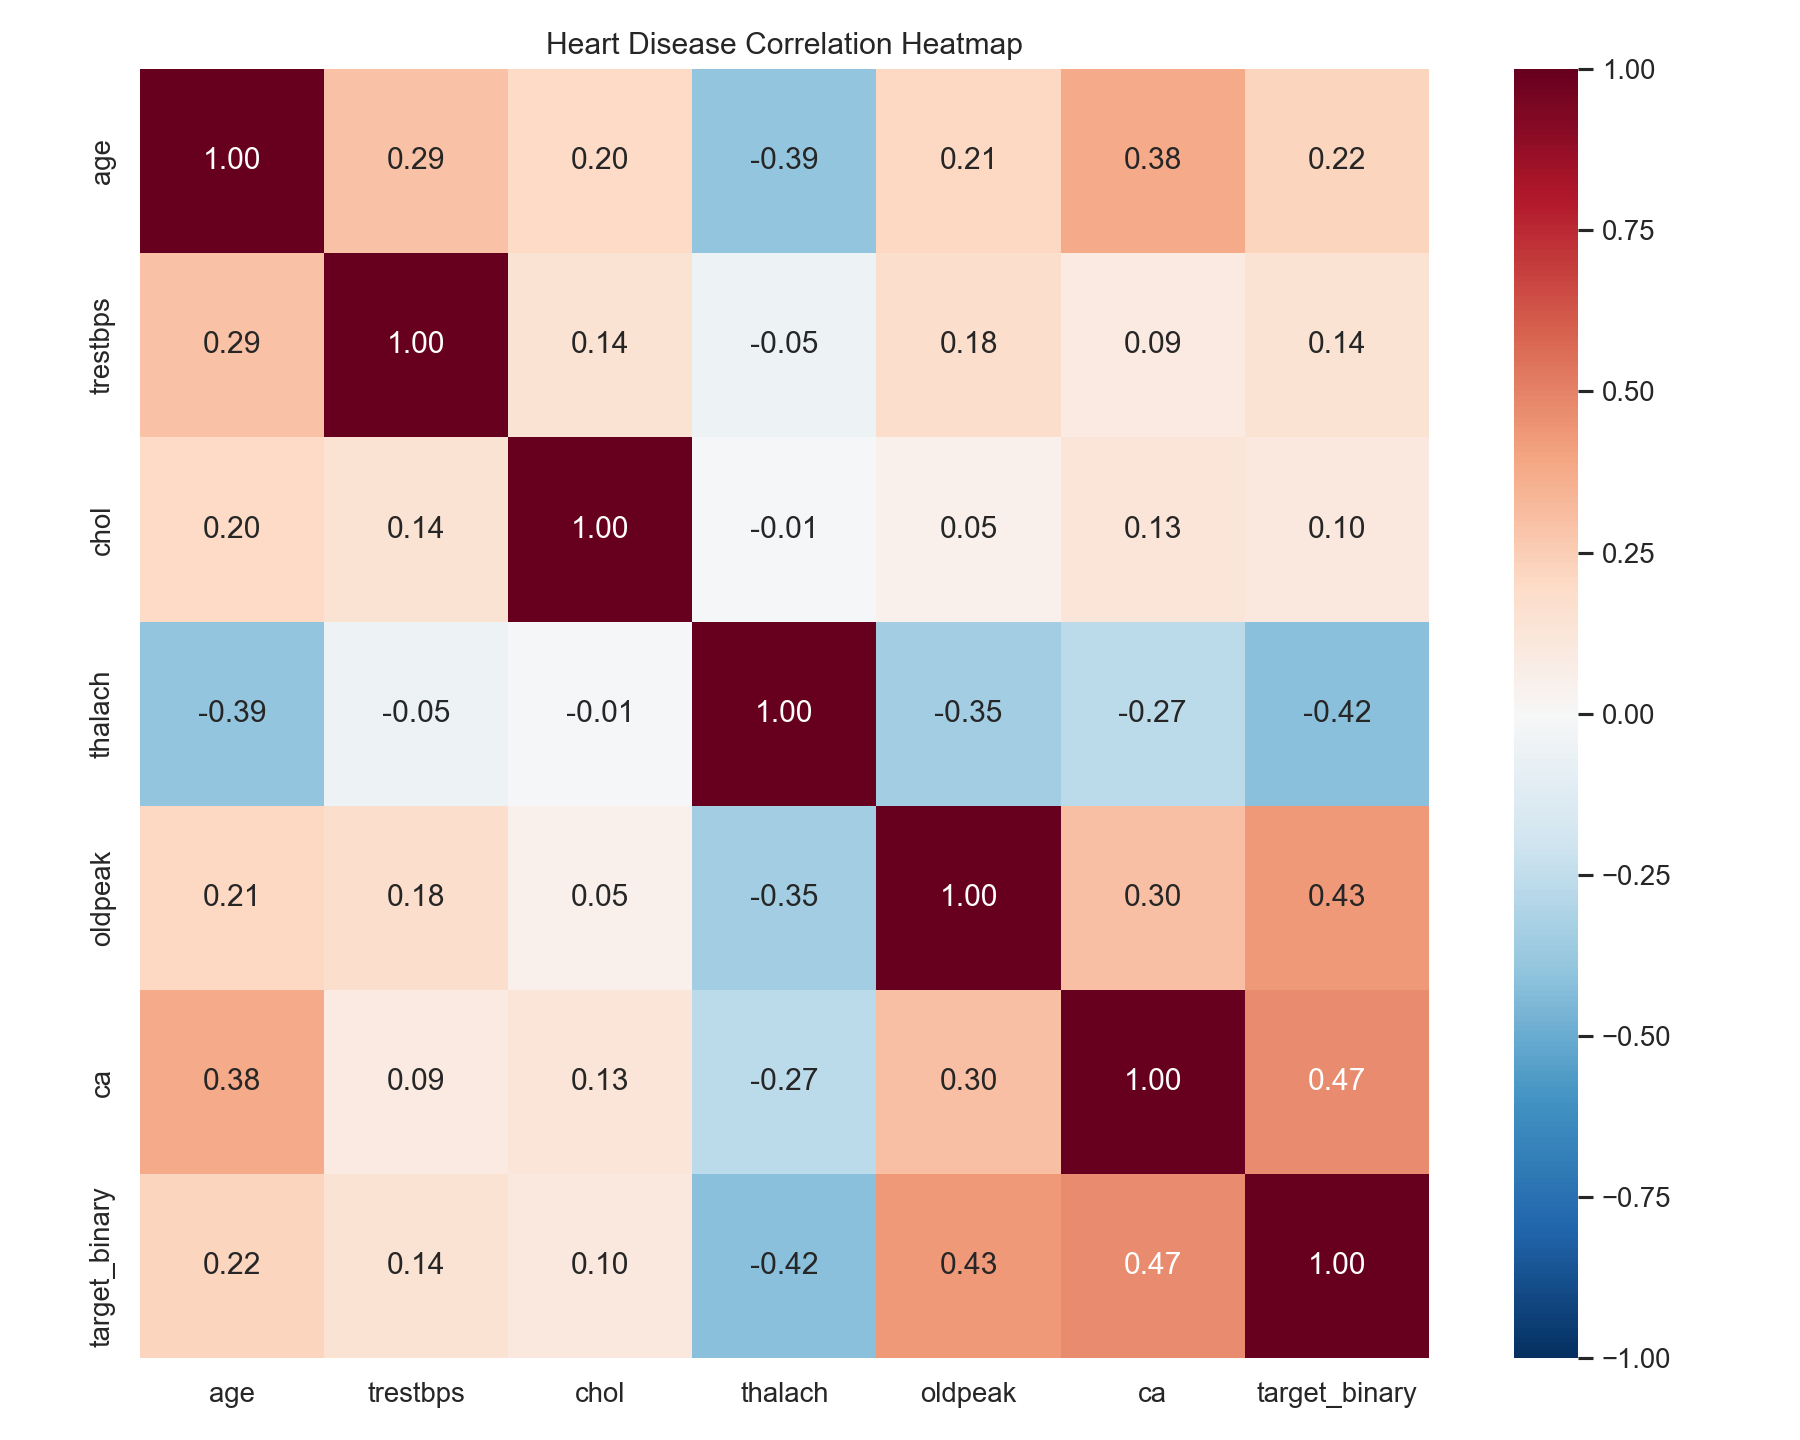
\includegraphics[width=0.95\textwidth]{images/ch1/heart_disease_correlation_heatmap.png}
\caption[Minh họa correlation heatmap Heart Disease]{Minh họa correlation heatmap: tương quan biến trong Heart Disease.}
\label{fig:chapter1_heatmap_example}
\end{figure}

\textbf{Nhận xét và lý do chọn.} Correlation heatmap được chọn vì Heart Disease có nhiều biến định lượng và cần xem nhanh quan hệ giữa nhiều cặp biến cùng lúc. Nếu chỉ dùng scatter plot, mỗi hình chỉ thể hiện một cặp biến; heatmap gom toàn bộ ma trận tương quan vào một hình, giúp phát hiện cặp biến có liên hệ dương/âm mạnh và các nhóm biến có khả năng trùng thông tin. Hình \ref{fig:chapter1_heatmap_example} phù hợp cho bước chọn đặc trưng trước khi học máy. Tuy nhiên, heatmap chỉ phản ánh tương quan tuyến tính, không chứng minh quan hệ nhân quả và không thay thế kiểm định thống kê hay kiến thức chuyên ngành y tế.

\textbf{Ghi chú về Excel.} Excel không có chart object heatmap riêng; workbook chỉ lưu ma trận tương quan ở sheet \texttt{Heart Corr} với conditional formatting, không nhúng ảnh preview. Vì vậy hình minh họa heatmap trong báo cáo được tính là biểu đồ Python.

\subsection{Một số dạng biểu đồ bổ sung phù hợp với bài toán}

Ngoài sáu dạng chính, báo cáo đề xuất thêm ba biểu đồ mới có khả năng bổ sung trực tiếp cho phân tích trong các chương sau: raincloud plot cho phân phối theo lớp, ridgeline plot cho nhiều phân phối song song và hexbin plot cho dữ liệu hai biến có mật độ điểm cao. Ba biểu đồ này không thay thế histogram, boxplot hoặc scatter plot; chúng được dùng khi biểu đồ cơ bản bắt đầu che mất mật độ, chồng điểm hoặc khác biệt nhỏ giữa nhiều nhóm. Các biểu đồ mới được khai báo trong Bảng \ref{tab:chapter1_extra_chart_types} trước khi minh họa chi tiết.

\begin{table}[H]
\centering
\caption{Đề xuất 3 biểu đồ mới: ưu điểm, nhược điểm và phạm vi áp dụng}
\label{tab:chapter1_extra_chart_types}
\small
\begin{tabular}{p{0.16\textwidth}p{0.25\textwidth}p{0.21\textwidth}p{0.21\textwidth}p{0.12\textwidth}}
\toprule
Biểu đồ mới & Giới thiệu & Ưu điểm & Nhược điểm & Phạm vi áp dụng \\
\midrule
Raincloud plot & Kết hợp density/violin, boxplot và điểm dữ liệu thô trong cùng một hình. & Vừa thấy hình dạng phân phối, median/IQR, vừa thấy từng quan sát; tốt hơn boxplot khi cần giải thích sự chồng lấn giữa các lớp. & Dễ rối nếu số lớp nhiều hoặc mẫu quá lớn; cần chú thích rõ để người đọc không quen vẫn hiểu. & So sánh biến định lượng theo lớp: \texttt{chol} theo \texttt{target\_binary}, độ sáng ảnh HAM10000 theo \texttt{dx}. \\
Ridgeline plot & Xếp nhiều density plot theo hàng ngang để so sánh nhiều nhóm hoặc nhiều mốc thời gian. & Tiết kiệm không gian khi có nhiều phân phối; dễ nhận ra dịch chuyển trung tâm, độ lệch và đa đỉnh giữa các nhóm. & Không phù hợp nếu nhóm quá ít; phần chồng lớp có thể gây hiểu nhầm diện tích nếu thang đo không thống nhất. & So sánh phân phối \texttt{Appliances} theo tháng/ngày trong tuần hoặc phân phối tuổi theo lớp bệnh. \\
Hexbin plot & Chia mặt phẳng hai biến thành các ô lục giác và tô màu theo số điểm trong mỗi ô. & Giải quyết overplotting tốt hơn scatter plot khi dữ liệu nhiều điểm; màu thể hiện mật độ quan sát. & Mất thông tin từng điểm; kết quả phụ thuộc kích thước ô và thang màu. & Cặp biến định lượng dày điểm: \texttt{T1}--\texttt{Appliances}, \texttt{age}--\texttt{thalach}, đặc trưng ảnh số hóa. \\
\bottomrule
\end{tabular}
\end{table}

\subsubsection{Raincloud plot (Biểu đồ mưa-mây) cho phân phối theo lớp}

Raincloud plot trong Bảng \ref{tab:chapter1_extra_chart_types} kết hợp ba lớp thông tin: density/violin để thấy hình dạng phân phối, boxplot để đọc median và IQR, và điểm jitter để thấy quan sát thô. Biểu đồ này phù hợp khi cần so sánh biến định lượng giữa các nhóm nhưng boxplot đơn lẻ chưa cho biết mật độ điểm tập trung ở đâu. Với Heart Disease, raincloud plot có thể dùng cho \texttt{chol} theo \texttt{target\_binary}. Dữ liệu đầu vào gồm hai cột: nhãn bệnh \texttt{target\_binary} và cholesterol \texttt{chol}; mỗi nhóm được vẽ một nửa density, một hộp IQR và các điểm jitter. Nếu nhóm có bệnh có đuôi phải dài hơn, biểu đồ cho thấy khác biệt không chỉ ở median mà còn ở mật độ và dữ liệu bất thường. \textbf{Hạn chế:} raincloud plot dễ rối khi có quá nhiều lớp hoặc quá nhiều điểm; cần chú thích rõ ý nghĩa của density, hộp IQR và điểm dữ liệu.

\subsubsection{Ridgeline plot (Biểu đồ sống núi) cho nhiều phân phối song song}

Ridgeline plot trong Bảng \ref{tab:chapter1_extra_chart_types} xếp nhiều đường mật độ theo từng nhóm hoặc từng mốc thời gian. Biểu đồ này phù hợp khi cần so sánh nhiều phân phối cùng lúc mà histogram hoặc KDE riêng lẻ chiếm quá nhiều không gian. Với Appliances Energy, ridgeline plot được dùng để so sánh phân phối \texttt{log1p(Appliances)} theo tháng. Dữ liệu đầu vào gồm tháng trích từ biến thời gian và giá trị \texttt{Appliances\_log1p}; mỗi tháng tạo một density riêng, xếp chồng theo trục dọc. Nếu một tháng có density lệch phải hơn tháng khác, người phân tích có cơ sở kiểm tra yếu tố mùa vụ hoặc thay đổi hành vi tiêu thụ. \textbf{Hạn chế:} ridgeline plot có thể gây hiểu nhầm nếu thang mật độ không thống nhất hoặc các đường chồng quá mạnh; nên dùng cùng thang đo và sắp xếp nhóm theo thời gian.

\begin{figure}[H]
\centering
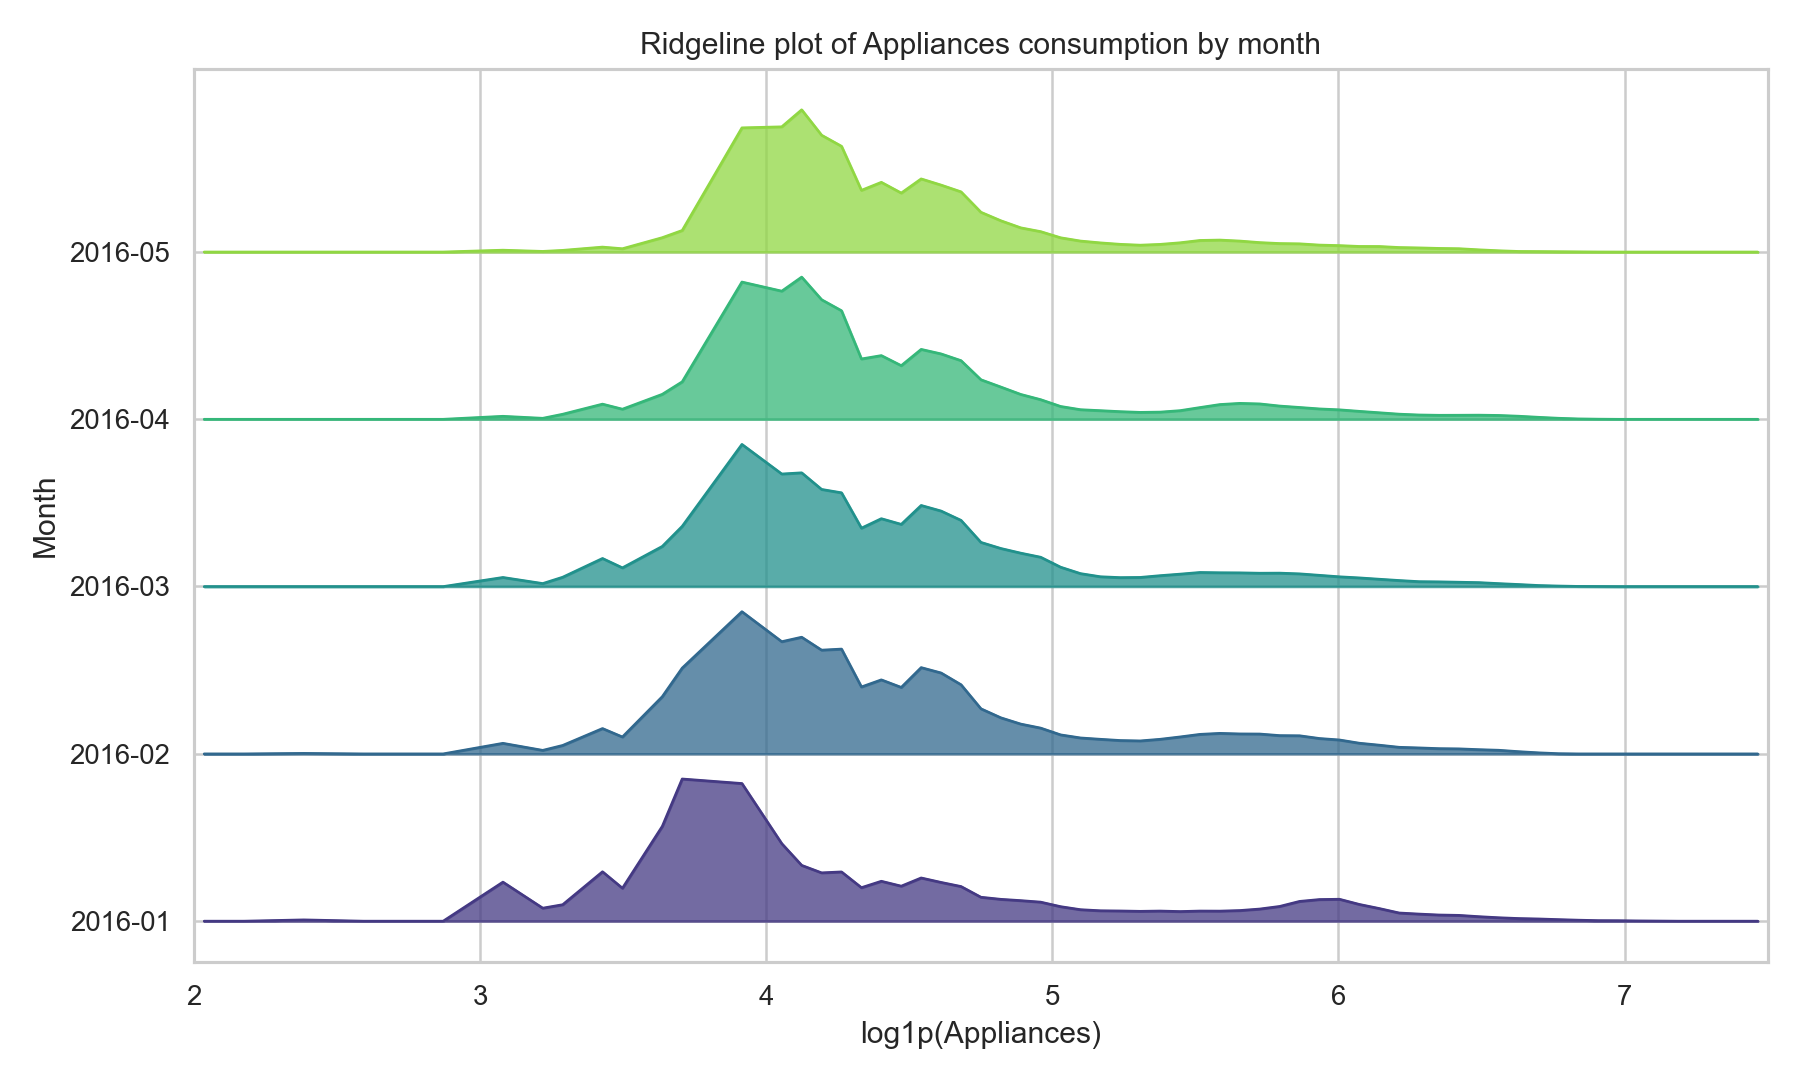
\includegraphics[width=0.92\textwidth]{images/ch1/appliances_energy_monthly_ridgeline.png}
\caption[Minh họa ridgeline Appliances Energy]{Minh họa ridgeline plot: phân phối \texttt{log1p(Appliances)} theo từng tháng.}
\label{fig:chapter1_ridgeline_example_inline}
\end{figure}

\textbf{Ghi chú về Excel.} Excel không có chart ridgeline native, nên báo cáo không xem ridgeline là biểu đồ Excel. Sheet \texttt{Appliances Ridgeline} chỉ lưu dữ liệu \texttt{month + log1p} để người đọc có thể dựng nhiều histogram theo tháng nếu cần; hình ridgeline trong báo cáo được render bằng Python.

\subsubsection{Hexbin plot (Biểu đồ tổ ong) cho dữ liệu hai biến dày điểm}

Hexbin plot trong Bảng \ref{tab:chapter1_extra_chart_types} chia mặt phẳng hai biến thành các ô lục giác và tô màu theo số quan sát trong từng ô. Biểu đồ này phù hợp khi scatter plot bị overplotting, tức nhiều điểm chồng lên nhau làm người đọc không thấy vùng mật độ cao. Với dữ liệu 19,735 mẫu của Appliances Energy, hexbin plot giữa \texttt{T1} và \texttt{Appliances} phù hợp hơn scatter plot vì mỗi ô màu đậm cho biết vùng nhiệt độ phòng và mức tiêu thụ điện xuất hiện thường xuyên. Với Heart Disease, hexbin cũng có thể dùng cho cặp \texttt{age}--\texttt{thalach} nếu mở rộng sang dữ liệu lớn hơn. \textbf{Hạn chế:} hexbin plot làm mất thông tin từng điểm riêng lẻ; kết quả phụ thuộc kích thước ô và thang màu, nên cần chọn tham số nhất quán khi so sánh nhiều hình.

\begin{table}[H]
\centering
\caption{Dữ liệu mẫu minh họa ba biểu đồ mới}
\label{tab:chapter1_extra_chart_sample_data}
\small
\begin{tabular}{lrrrr}
\toprule
Dataset & Biến nhóm/thời gian & Biến $x$ & Biến $y$ & Biểu đồ phù hợp \\
\midrule
Heart Disease & \texttt{target\_binary} & -- & \texttt{chol} & Raincloud plot \\
Heart Disease & \texttt{target\_binary} & -- & \texttt{thalach} & Raincloud plot \\
Appliances Energy & Tháng/ngày trong tuần & -- & \texttt{Appliances} & Ridgeline plot \\
Appliances Energy & -- & \texttt{T1} & \texttt{Appliances} & Hexbin plot \\
HAM10000 & \texttt{dx} & -- & Mean intensity & Raincloud/Ridgeline plot \\
\bottomrule
\end{tabular}
\end{table}

\begin{figure}[H]
\centering
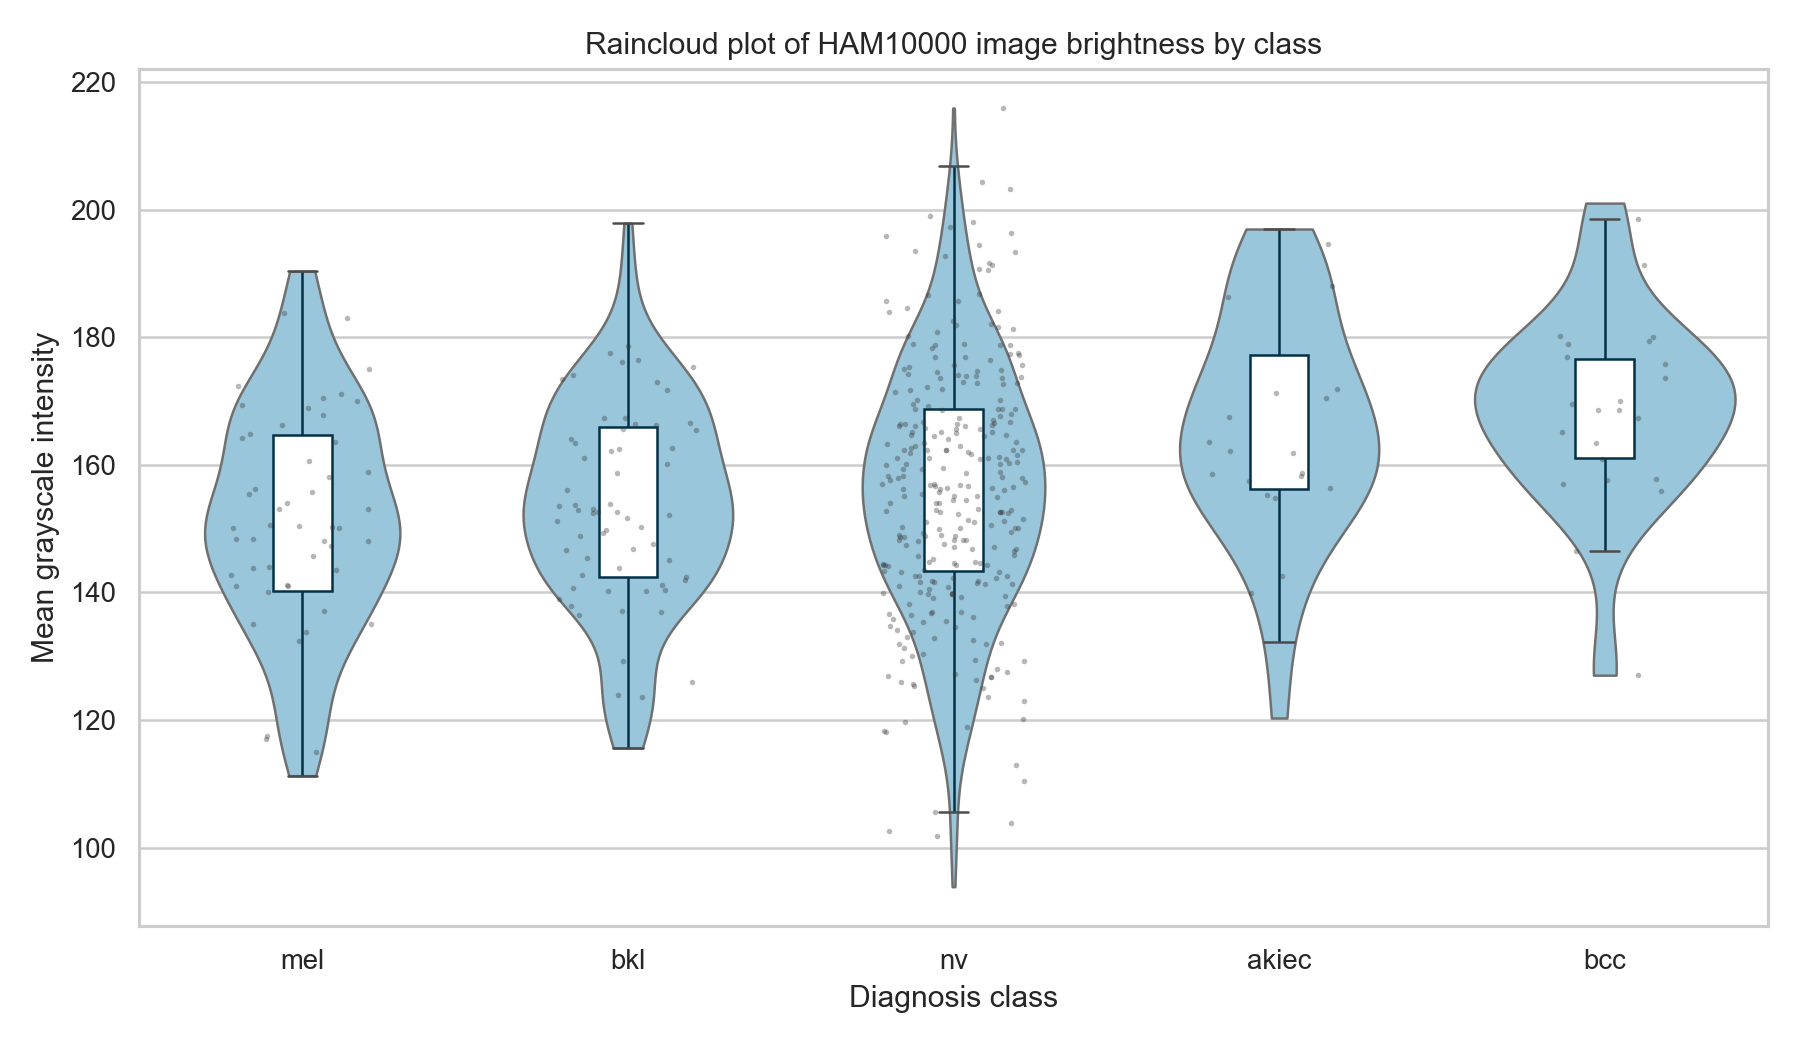
\includegraphics[width=0.90\textwidth]{images/ch1/ham10000_mean_intensity_raincloud.png}
\caption[Minh họa raincloud plot HAM10000]{Biểu đồ mưa-mây (Raincloud plot) thể hiện đồng thời phân phối mật độ nhân (KDE), biểu đồ hộp và phân phối điểm của độ sáng ảnh theo lớp.}
\label{fig:chapter1_extra_chart_examples}
\end{figure}

\begin{figure}[H]
\centering
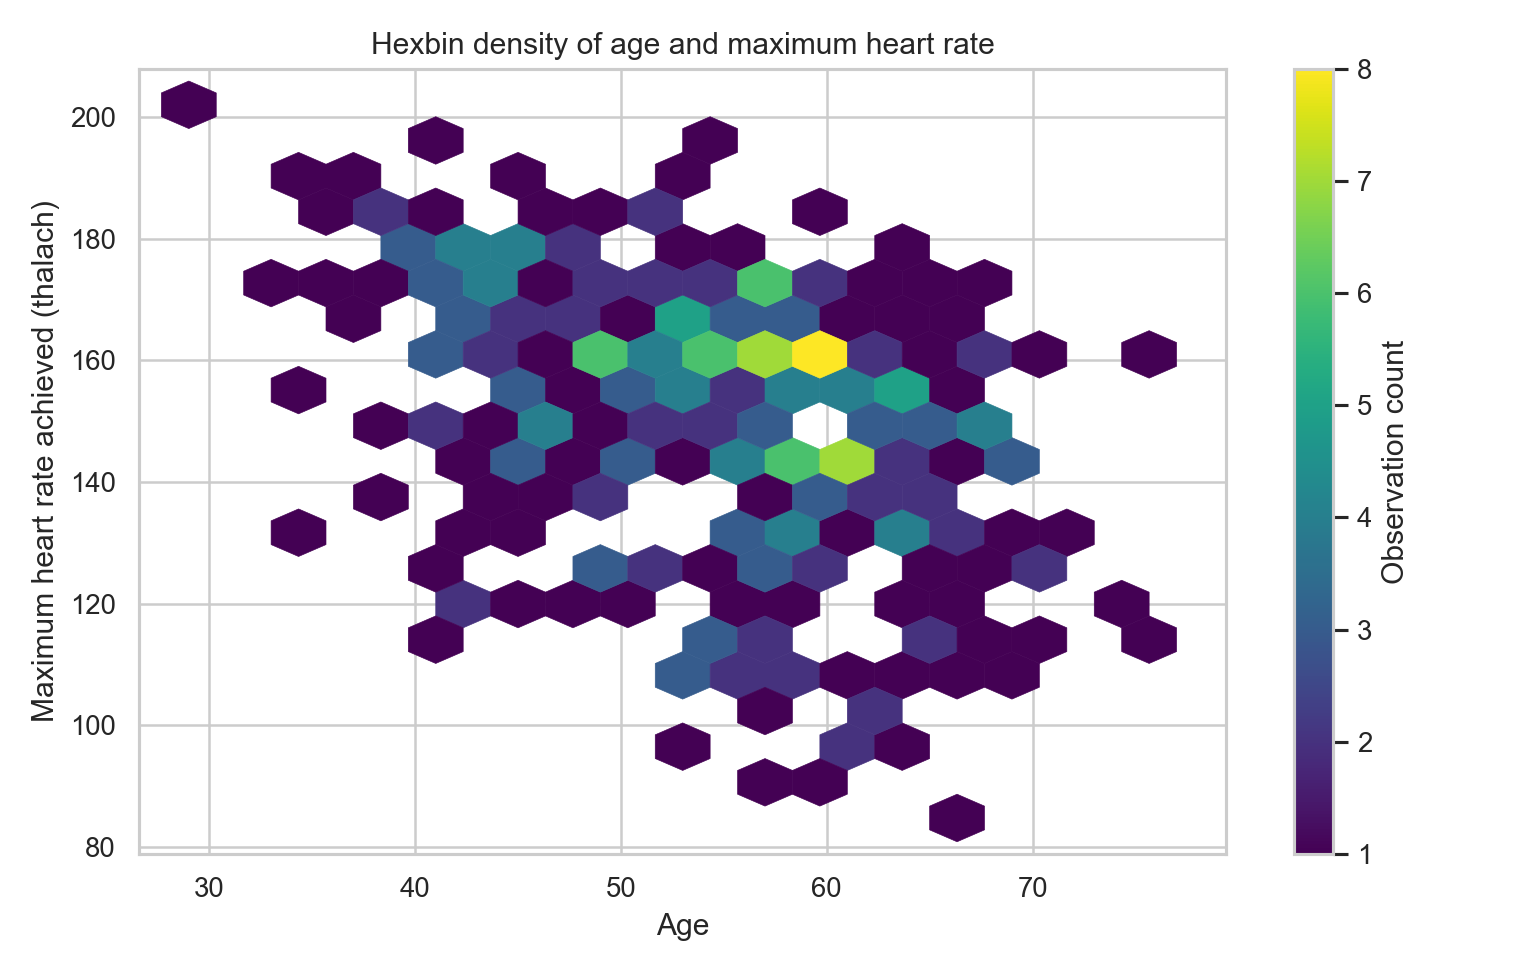
\includegraphics[width=0.90\textwidth]{images/ch1/heart_age_thalach_hexbin.png}
\caption[Minh họa hexbin plot Heart Disease]{Biểu đồ tổ ong (Hexbin plot) thể hiện mật độ phân bố đồng thời của thuộc tính Tuổi và Nhịp tim tối đa, giúp khắc phục hiện tượng chồng lấp điểm dữ liệu.}
\label{fig:chapter1_extra_chart_examples_hexbin}
\end{figure}

\textbf{Nhận xét và lý do chọn.} Ba biểu đồ mới được chọn vì mỗi biểu đồ xử lý một hạn chế cụ thể của biểu đồ cơ bản. Raincloud plot mở rộng boxplot khi cần thấy cả density và điểm dữ liệu; ridgeline plot mở rộng KDE khi cần so sánh nhiều nhóm/thời đoạn; hexbin plot mở rộng scatter plot khi điểm quan sát quá dày. Trong báo cáo, chúng nên được dùng có chọn lọc: chỉ thêm khi câu hỏi phân tích cần mật độ phân phối, nhiều nhóm song song hoặc dữ liệu hai biến quá đông điểm. Nếu mục tiêu chỉ là mô tả đơn giản, histogram, boxplot và scatter plot vẫn là lựa chọn dễ đọc hơn.

\section{Các phép biến đổi và tiền xử lý cơ bản}

Các phép biến đổi và tiền xử lý là cầu nối giữa thống kê mô tả và mô hình hóa. Theo Han, Kamber và Pei, chất lượng dữ liệu ảnh hưởng trực tiếp đến chất lượng khai phá dữ liệu; dữ liệu thiếu, nhiễu, lệch thang đo hoặc không dừng có thể làm mô hình học sai cấu trúc thật \cite{Han2011DataMining}. Trong học máy ứng dụng, Kuhn và Johnson cũng nhấn mạnh rằng tiền xử lý và feature engineering phải được quyết định dựa trên bản chất biến, phân phối và thuật toán sử dụng, không nên áp dụng máy móc cho mọi cột \cite{Kuhn2019FeatureEngineering}. Với dữ liệu chuỗi thời gian, Hyndman và Athanasopoulos khuyến nghị xử lý biến đổi phương sai, sai phân và kiểm tra thứ tự thời gian trước khi dự báo \cite{Hyndman2021Forecasting}.

\subsection{Điền khuyết}

Dữ liệu thực tế thường có missing value do lỗi nhập liệu, lỗi cảm biến, file bị ghép thiếu hoặc một số thuộc tính không đo được ở mọi mẫu. Nếu bỏ toàn bộ dòng thiếu, kích thước mẫu có thể giảm mạnh và tạo thiên lệch nếu missing không ngẫu nhiên. Vì vậy, cần chọn cách điền khuyết theo kiểu biến và nguyên nhân thiếu. Với biến định lượng cân bằng, mean giữ nguyên trung bình tổng thể; với biến định lượng lệch hoặc có dữ liệu bất thường, median bền vững hơn; với biến định tính, mode giữ lại lớp phổ biến nhất.

\begin{equation}
x_{missing} =
\begin{cases}
median(X), & \text{nếu X là biến định lượng có dữ liệu bất thường} \\
mean(X), & \text{nếu X là biến định lượng cân bằng} \\
mode(X), & \text{nếu X là biến định tính}
\end{cases}
\end{equation}

\textbf{Trường hợp/phạm vi áp dụng.} Điền mean/median phù hợp khi tỷ lệ thiếu thấp và biến thiếu không phải nhãn mục tiêu. Điền mode phù hợp với biến phân loại có số lớp ít. Với chuỗi thời gian, nên ưu tiên nội suy, forward fill hoặc backward fill nếu giá trị liền kề có ý nghĩa thời gian. Không nên điền khuyết tùy tiện khi tỷ lệ thiếu quá cao, khi missing mang ý nghĩa riêng, hoặc khi biến thiếu là target cần dự báo.

\textbf{Ví dụ cụ thể.} Trong Heart Disease, biến \texttt{ca} thiếu 4 giá trị và \texttt{thal} thiếu 2 giá trị. Vì tỷ lệ thiếu thấp, có thể điền \texttt{ca} bằng median/mode sau khi xem phân phối, và điền \texttt{thal} bằng mode vì đây là biến phân loại được mã hóa. Trong Appliances Energy, các biến cảm biến nếu có khoảng trống ngắn nên dùng nội suy tuyến tính theo thời gian để giữ xu hướng liên tục thay vì điền mean toàn cục.

\subsection{Chuẩn hóa thang đo}

Trong học máy, các biến có thang đo khác nhau có thể làm thuật toán dựa trên khoảng cách hoặc gradient bị lệch. Ví dụ, cholesterol có miền khoảng hàng trăm, còn \texttt{oldpeak} chỉ khoảng 0--6; nếu dùng K-Means hoặc SVM mà không chuẩn hóa, biến có đơn vị lớn dễ chi phối khoảng cách. Hai kỹ thuật cơ bản là min-max scaling và standardization.

Min-max scaling đưa giá trị về khoảng $[0,1]$:

\begin{equation}
x' = \frac{x - x_{min}}{x_{max} - x_{min}}
\end{equation}

Standardization đưa dữ liệu về mean 0 và standard deviation 1:

\begin{equation}
x' = \frac{x - \mu}{\sigma}
\end{equation}

\textbf{Trường hợp/phạm vi áp dụng.} Min-max scaling phù hợp khi cần giữ miền cố định, ví dụ đặc trưng ảnh đưa về $[0,1]$ hoặc mô hình neural network. Standardization phù hợp hơn cho Logistic Regression, SVM, PCA, K-Means và Hierarchical Clustering vì các thuật toán này nhạy với thang đo. Không bắt buộc chuẩn hóa cho cây quyết định và Random Forest vì chúng tách theo ngưỡng từng biến, nhưng chuẩn hóa vẫn có thể hữu ích khi so sánh hệ số hoặc kết hợp với thuật toán khác.

\textbf{Ví dụ cụ thể.} Với Heart Disease, trước khi chạy K-Means, các biến \texttt{age}, \texttt{trestbps}, \texttt{chol}, \texttt{thalach}, \texttt{oldpeak} cần standardization để \texttt{chol} không áp đảo khoảng cách. Với HAM10000, nếu trích đặc trưng độ sáng trung bình từ ảnh, giá trị pixel nên chia cho 255 để đưa về $[0,1]$ trước khi so sánh giữa ảnh.

\subsection{Log transform và differencing cho chuỗi thời gian}
\label{sec:logtransform}

Log transform dùng khi biến định lượng lệch phải mạnh, có nhiều giá trị nhỏ nhưng một số giá trị rất lớn. Phép biến đổi này nén phần đuôi phải, giảm ảnh hưởng của giá trị cực trị và giúp mô hình tuyến tính dễ học hơn. Với dữ liệu chuỗi thời gian, log transform còn giúp phương sai ổn định hơn trước khi dự báo \cite{Hyndman2021Forecasting}:

\begin{equation}
y'_t = \log(1 + y_t)
\end{equation}

Sai phân bậc 1 giúp loại bỏ xu hướng cục bộ và chuyển phân tích từ mức giá trị sang mức thay đổi:

\begin{equation}
\Delta y_t = y_t - y_{t-1}
\end{equation}

\textbf{Trường hợp/phạm vi áp dụng.} Log1p phù hợp với biến không âm và lệch phải như \texttt{Appliances}, chi phí, doanh thu, số lượt truy cập hoặc cường độ pixel tổng hợp. Không dùng log trực tiếp cho giá trị âm; khi có 0 nên dùng \texttt{log1p}. Differencing phù hợp cho chuỗi thời gian có xu hướng hoặc mức nền thay đổi; tuy nhiên nếu sai phân quá mức có thể làm mất thông tin dài hạn và tăng nhiễu.

\textbf{Ví dụ cụ thể.} Trong Appliances Energy, \texttt{Appliances\_log1p} và \texttt{Appliances\_diff} đã được tạo trong script \texttt{src/analyze\_appliances\_energy.py}. Histogram raw cho thấy \texttt{Appliances} lệch phải, còn histogram log1p gọn hơn. Line chart theo ngày và ridgeline plot theo tháng giúp kiểm tra liệu phân phối tiêu thụ điện có thay đổi theo thời gian hay không. Khi xây dựng mô hình dự báo, dữ liệu phải chia train/test theo thứ tự thời gian, không random split, để tránh rò rỉ thông tin tương lai.

\begin{table}[H]
\centering
\caption{Tóm tắt phạm vi áp dụng các phép tiền xử lý cơ bản}
\label{tab:chapter1_preprocess_scope}
\small
\begin{tabular}{p{0.18\textwidth}p{0.27\textwidth}p{0.25\textwidth}p{0.20\textwidth}}
\toprule
Kỹ thuật & Áp dụng khi & Không nên dùng khi & Ví dụ trong báo cáo \\
\midrule
Mean/median/mode imputation & Tỷ lệ thiếu thấp, biến đầu vào quan trọng & Missing quá cao hoặc missing là tín hiệu riêng & \texttt{ca}, \texttt{thal} trong Heart Disease \\
Nội suy thời gian & Chuỗi thời gian có khoảng trống ngắn & Khoảng trống dài, cảm biến lỗi kéo dài & Cảm biến Appliances Energy \\
Min-max scaling & Cần miền $[0,1]$, dữ liệu ảnh/neural network & Có dữ liệu bất thường mạnh chưa xử lý & Độ sáng ảnh HAM10000 \\
Standardization & SVM, Logistic Regression, PCA, K-Means & Cần giữ đơn vị gốc để giải thích trực tiếp & Các biến Heart Disease trước clustering \\
Log1p transform & Biến không âm lệch phải & Dữ liệu âm hoặc cần diễn giải đơn vị gốc & \texttt{Appliances\_log1p} \\
Differencing & Chuỗi có xu hướng, cần phân tích thay đổi & Chuỗi quá nhiễu hoặc cần mức tuyệt đối & \texttt{Appliances\_diff} \\
\bottomrule
\end{tabular}
\end{table}

\section{Quy trình phân tích khám phá dữ liệu}

Phân tích khám phá dữ liệu (Exploratory Data Analysis - EDA) là giai đoạn nối giữa dữ liệu thô và mô hình phân tích. Nếu bỏ qua EDA, người phân tích có thể đưa vào mô hình các biến bị lỗi kiểu dữ liệu, phân phối lệch quá mạnh, chứa dữ liệu bất thường bất thường hoặc có target mất cân bằng. Trong báo cáo này, EDA được xem như một quy trình có kiểm soát gồm năm bước.

\begin{enumerate}[leftmargin=2.2em,label=\textbf{\arabic*.}]
 \item \textbf{Kiểm tra cấu trúc dữ liệu}: xác định số dòng, số cột, kiểu dữ liệu, khóa thời gian, nhãn mục tiêu và các file nguồn.
 \item \textbf{Kiểm tra chất lượng dữ liệu}: tìm giá trị thiếu, giá trị trùng, giá trị ngoài miền hợp lý và kiểu dữ liệu bị đọc sai.
 \item \textbf{Thống kê mô tả}: tính mean, median, mode, percentile, variance, standard deviation, CV và IQR cho các biến định lượng; lập bảng tần suất cho biến định tính.
 \item \textbf{Trực quan hóa}: chọn biểu đồ phù hợp với bản chất biến và câu hỏi phân tích.
 \item \textbf{Rút kết luận phân tích}: ghi nhận đặc điểm dữ liệu có ảnh hưởng đến tiền xử lý, feature engineering và mô hình học máy.
\end{enumerate}

Điểm quan trọng là EDA không dừng ở việc tạo ra nhiều hình. Mỗi hình phải trả lời một câu hỏi cụ thể. Ví dụ, histogram trả lời câu hỏi ``biến này phân phối như thế nào?'', boxplot trả lời câu hỏi ``biến này có dữ liệu bất thường không?'', scatter plot trả lời câu hỏi ``hai biến có quan hệ gì không?'', còn line chart trả lời câu hỏi ``dữ liệu thay đổi ra sao theo thời gian?''.

\begin{table}[H]
\centering
\caption{Quy trình EDA và sản phẩm đầu ra cần lưu}
\label{tab:chapter1_eda_outputs}
\small
\begin{tabular}{p{0.20\textwidth}p{0.32\textwidth}p{0.34\textwidth}}
\toprule
Bước & Câu hỏi chính & Sản phẩm đầu ra \\
\midrule
Kiểm kê dữ liệu & Dữ liệu có bao nhiêu dòng/cột? & Inventory CSV, mô tả dataset \\
Kiểm tra thiếu & Biến nào thiếu và thiếu bao nhiêu? & Missing-value table \\
Thống kê mô tả & Trung tâm và độ phân tán ra sao? & Summary table \\
Trực quan hóa & Phân phối, dữ liệu bất thường, quan hệ biến thế nào? & PNG figure, Excel chart \\
Diễn giải & Kết quả tác động gì đến mô hình? & Nhận xét trong báo cáo \\
\bottomrule
\end{tabular}
\end{table}

Bảng \ref{tab:chapter1_eda_outputs} cũng là cơ sở tổ chức thư mục của dự án. Các file trong \texttt{outputs/tables/} lưu bằng chứng dạng bảng; các file trong \texttt{outputs/figures/} lưu biểu đồ; các file trong \texttt{src/} lưu script tạo kết quả. Cách tổ chức này giúp báo cáo không chỉ có kết luận, mà còn có đường dẫn tái lập kết luận.

\section{Nguyên tắc chọn biểu đồ theo câu hỏi phân tích}

Không có một loại biểu đồ nào phù hợp cho mọi dữ liệu. Việc chọn biểu đồ phụ thuộc vào loại biến, số biến cần so sánh và câu hỏi đang đặt ra. Nếu chọn sai biểu đồ, người đọc có thể hiểu sai bản chất dữ liệu. Ví dụ, dùng pie chart cho biến có quá nhiều lớp sẽ khó so sánh; dùng scatter plot cho biến định tính sẽ không có ý nghĩa; dùng line chart cho dữ liệu không có thứ tự thời gian có thể tạo cảm giác có xu hướng giả.

\begin{table}[H]
\centering
\caption{Chọn biểu đồ theo loại câu hỏi phân tích}
\label{tab:chapter1_chart_by_question}
\small
\begin{tabular}{p{0.24\textwidth}p{0.26\textwidth}p{0.34\textwidth}}
\toprule
Câu hỏi phân tích & Biểu đồ ưu tiên & Lý do sử dụng \\
\midrule
Biến định lượng phân phối thế nào? & Histogram & Nhìn được dạng lệch, nhiều đỉnh, tập trung \\
Có dữ liệu bất thường không? & Boxplot & Dựa trên median, IQR và điểm ngoài ngưỡng \\
Hai biến số có quan hệ không? & Scatter plot & Thể hiện từng cặp quan sát trên mặt phẳng \\
Biến định tính có cơ cấu ra sao? & Bar chart & So sánh tần suất giữa các lớp rõ hơn pie chart \\
Dữ liệu thay đổi theo thời gian thế nào? & Line chart & Giữ thứ tự thời gian và phát hiện xu hướng \\
Nhiều biến liên hệ với nhau ra sao? & Correlation heatmap & Tóm tắt ma trận tương quan bằng màu sắc \\
\bottomrule
\end{tabular}
\end{table}

Trong báo cáo này, nguyên tắc chọn biểu đồ được áp dụng nhất quán. Với Heart Disease, histogram và boxplot được dùng để minh họa phân phối và dữ liệu bất thường; scatter plot và heatmap được dùng để khảo sát quan hệ biến. Với Appliances Energy, line chart là bắt buộc vì dữ liệu có trục thời gian. Với HAM10000, bar chart được dùng cho phân phối lớp, còn boxplot được dùng cho đặc trưng độ sáng sau khi số hóa ảnh.

\section{Diễn giải thống kê trong bối cảnh dữ liệu}

Một chỉ số thống kê chỉ có ý nghĩa khi được đọc trong bối cảnh dữ liệu. Mean không chỉ là một con số trung bình; nó cho biết mức đại diện nếu phân phối tương đối cân bằng. Median không chỉ là vị trí giữa; nó giúp so sánh với mean để nhận biết độ lệch. Standard deviation không chỉ đo độ phân tán; nó còn cho biết biến nào có dao động lớn và có thể cần chuẩn hóa. IQR không chỉ phục vụ boxplot; nó là nền tảng của quy tắc phát hiện dữ liệu bất thường.

Khi đọc một biến định lượng, báo cáo sử dụng ba lớp nhận xét:

\begin{itemize}[leftmargin=1.6em,label=\textbullet]
 \item \textbf{Nhận xét trung tâm}: mean và median gần hay xa nhau, biến có nghiêng lệch hay không.
 \item \textbf{Nhận xét phân tán}: standard deviation, range, IQR lớn hay nhỏ so với mean.
 \item \textbf{Nhận xét tiền xử lý}: có cần cắt dữ liệu bất thường, log-transform, chuẩn hóa hay không.
\end{itemize}

Ví dụ, trong Appliances Energy, mean của \texttt{Appliances} lớn hơn median và max rất cao, cho thấy target lệch phải. Nhận xét này dẫn trực tiếp đến việc dùng \texttt{log1p}. Ngược lại, trong Heart Disease, median của \texttt{chol} gần như không đổi trước và sau tiền xử lý, trong khi max giảm mạnh; điều này cho thấy tiền xử lý chủ yếu làm giảm ảnh hưởng của điểm cực trị, không làm thay đổi phần lõi của phân phối.

\section{Các sai lệch thường gặp khi đọc biểu đồ}

Trực quan hóa giúp dữ liệu dễ hiểu hơn, nhưng cũng có thể gây hiểu nhầm nếu không đọc đúng. Một số sai lệch thường gặp trong báo cáo dữ liệu gồm:

\begin{itemize}[leftmargin=1.6em,label=\textbullet]
 \item \textbf{Nhầm tương quan với nhân quả}: heatmap chỉ cho biết hai biến thay đổi cùng nhau, không chứng minh biến này gây ra biến kia.
 \item \textbf{Đánh giá mô hình chỉ bằng accuracy}: nếu target mất cân bằng, accuracy cao có thể chỉ do mô hình dự đoán lớp đa số.
 \item \textbf{Bỏ qua scale}: các biến có thang đo khác nhau làm scatter plot và thuật toán khoảng cách khó diễn giải nếu chưa chuẩn hóa.
 \item \textbf{Dùng biểu đồ tổng thể thay cho phân tích theo lớp}: phân phối toàn bộ dữ liệu có thể che mất khác biệt giữa các nhóm target.
 \item \textbf{Không gắn biểu đồ với câu hỏi}: một hình đẹp nhưng không trả lời câu hỏi phân tích thì không giúp cải thiện báo cáo.
\end{itemize}

Do đó, mỗi biểu đồ trong báo cáo được viết kèm lý do chọn biểu đồ và nhận xét. Cách trình bày này giúp người đọc hiểu không chỉ biểu đồ thể hiện gì, mà còn vì sao nó cần thiết cho bài toán phân tích dữ liệu.

\section{Minh họa tính toán trên Heart Disease}

Bộ Heart Disease Cleveland có 303 mẫu và 14 thuộc tính gốc được dùng phổ biến trong các thực nghiệm. Trong quá trình đọc dữ liệu, ký hiệu \texttt{?} được chuyển thành missing value. Bảng missing cho thấy biến \texttt{ca} thiếu 4 giá trị, tương đương 1.3201\%, và biến \texttt{thal} thiếu 2 giá trị, tương đương 0.6601\%.

\begin{table}[H]
\centering
\caption{Ví dụ thống kê mô tả trên một số biến Heart Disease}
\label{tab:chapter1_heart_stats}
\begin{tabular}{lrrrrr}
\toprule
Biến & Mean & Median & Std & Min & Max \\
\midrule
age & 54.44 & 56.00 & 9.04 & 29.00 & 77.00 \\
trestbps & 131.69 & 130.00 & 17.60 & 94.00 & 200.00 \\
chol & 246.69 & 241.00 & 51.78 & 126.00 & 564.00 \\
thalach & 149.61 & 153.00 & 22.88 & 71.00 & 202.00 \\
oldpeak & 1.04 & 0.80 & 1.16 & 0.00 & 6.20 \\
\bottomrule
\end{tabular}
\end{table}

Từ Bảng \ref{tab:chapter1_heart_stats}, có thể rút ra ba nhận xét ban đầu. Thứ nhất, biến \texttt{age} có median 56 và mean 54.44, cho thấy phân phối tuổi hơi nghiêng về nhóm trung niên và cao tuổi. Thứ hai, \texttt{chol} có range rất lớn, từ 126 đến 564, nên cần kiểm tra dữ liệu bất thường bằng boxplot. Thứ ba, \texttt{oldpeak} có median 0.8 nhưng mode 0.0, cho thấy một phần đáng kể bệnh nhân không có ST depression.

\begin{table}[H]
\centering
\caption{So sánh trước và sau tiền xử lý trên Heart Disease}
\label{tab:chapter1_preprocess_compare}
\small
\begin{tabular}{lrrrr}
\toprule
Biến & Mean thô & Mean sạch & Std thô & Std sạch \\
\midrule
trestbps & 131.69 & 131.35 & 17.60 & 16.65 \\
chol & 246.69 & 245.58 & 51.78 & 47.56 \\
thalach & 149.61 & 149.65 & 22.88 & 22.73 \\
oldpeak & 1.04 & 1.02 & 1.16 & 1.11 \\
ca & 0.67 & 0.63 & 0.94 & 0.86 \\
\bottomrule
\end{tabular}
\end{table}

Bảng \ref{tab:chapter1_preprocess_compare} cho thấy tiền xử lý không làm thay đổi mạnh giá trị trung tâm, nhưng làm giảm độ biến động của các biến có dữ liệu bất thường. Trường hợp rõ nhất là \texttt{chol}: standard deviation giảm từ 51.78 xuống 47.56, max giảm từ 564 xuống 371. Điều này phù hợp với mục tiêu của tiền xử lý: giữ lại cấu trúc chính của dữ liệu nhưng hạn chế ảnh hưởng của điểm cực trị.

\begin{figure}[H]
\centering
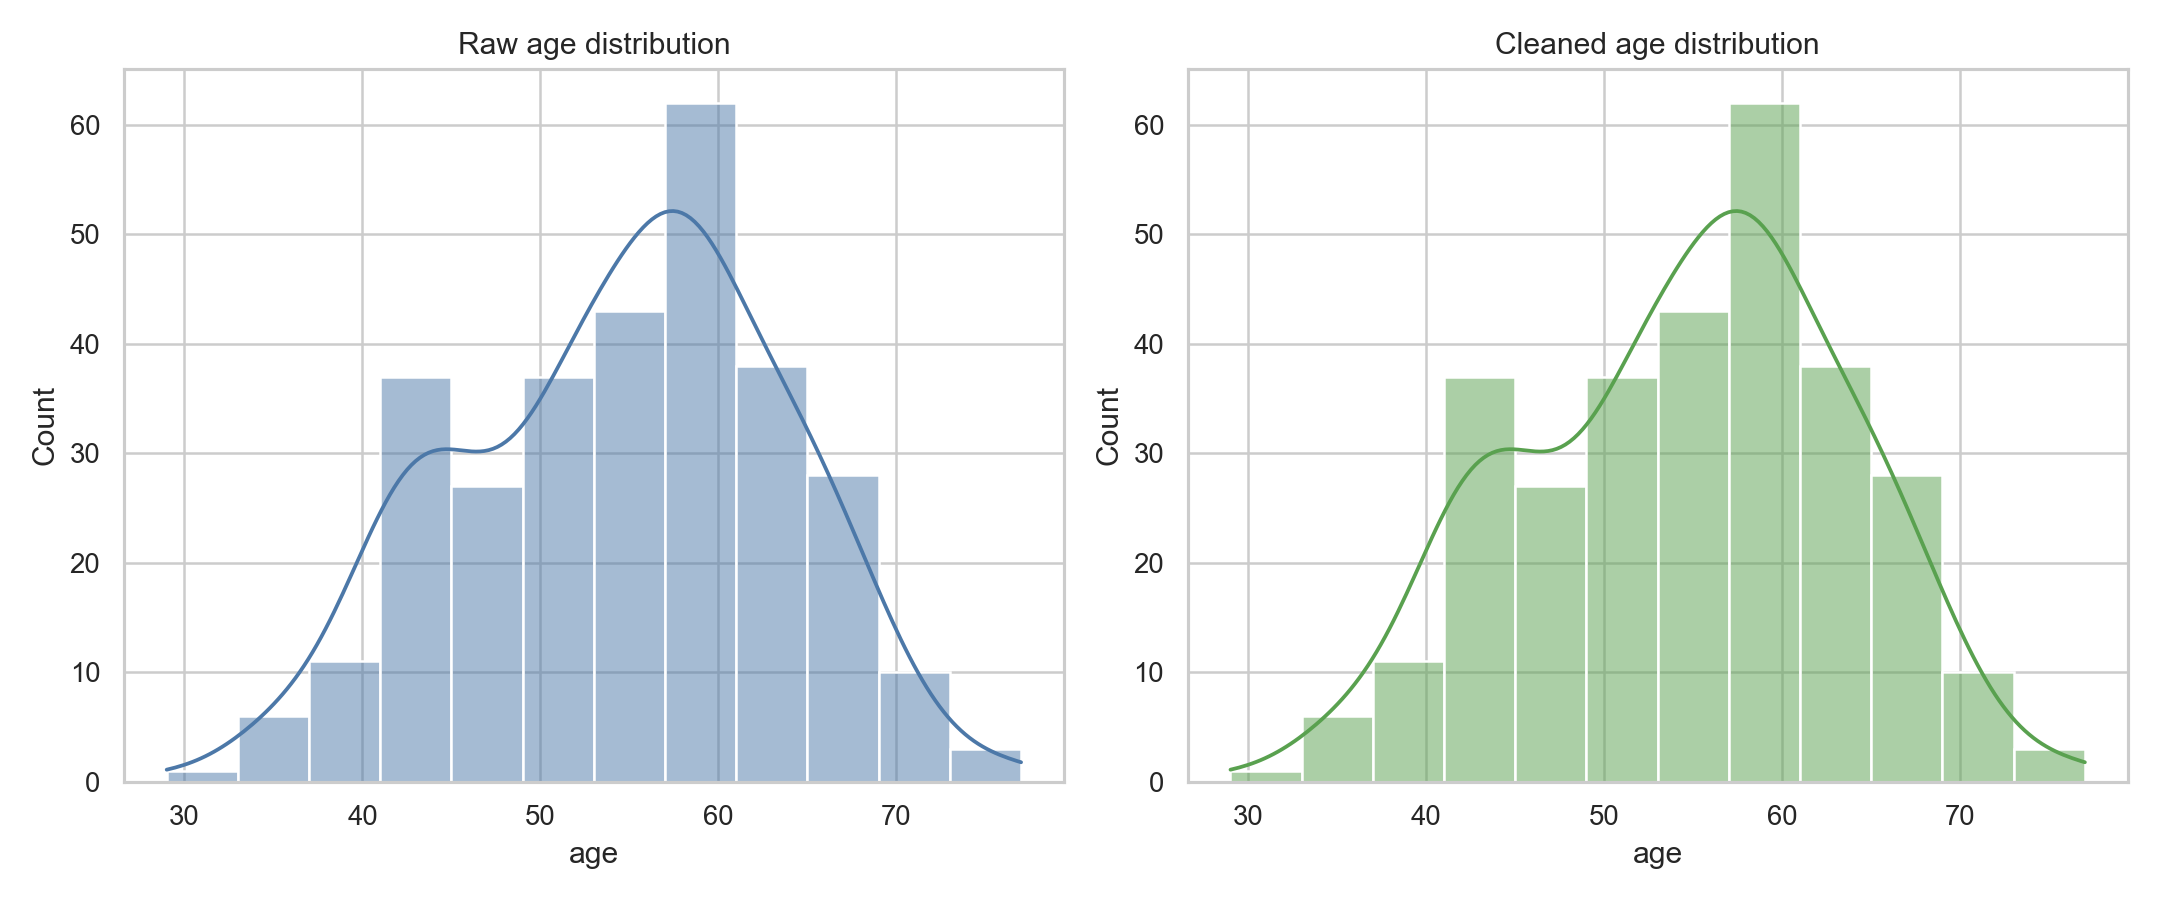
\includegraphics[width=0.90\textwidth]{images/ch1/heart_disease_age_raw_vs_cleaned.png}
\caption[Ví dụ histogram tuổi trên Heart Disease]{Ví dụ histogram tuổi trước/sau xử lý trên Heart Disease.}
\label{fig:chapter1_hist_box}
\end{figure}

\begin{figure}[H]
\centering
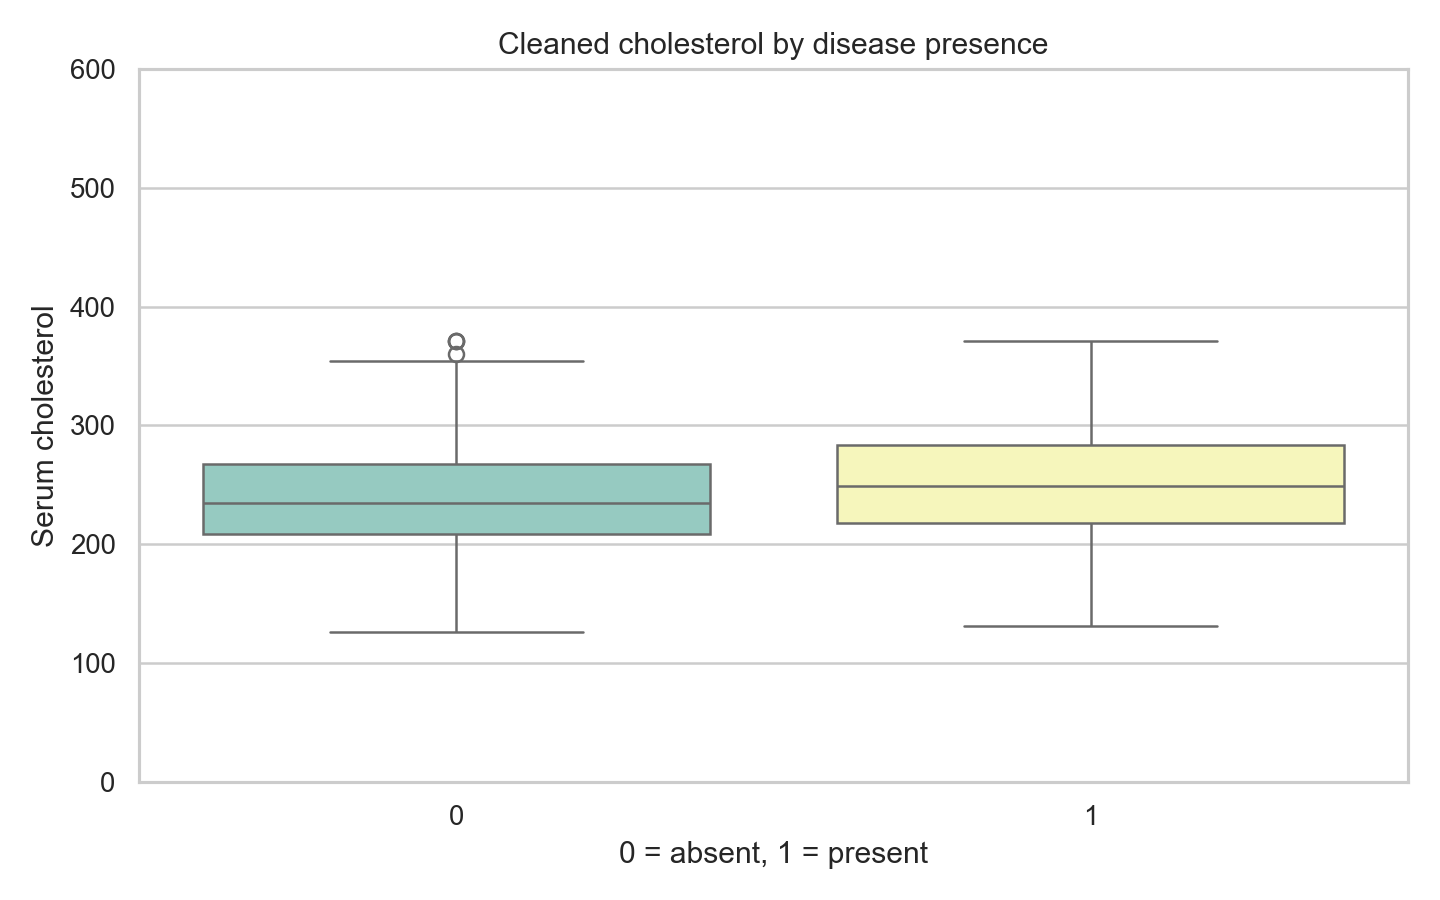
\includegraphics[width=0.90\textwidth]{images/ch1/heart_disease_cholesterol_boxplot.png}
\caption[Ví dụ boxplot cholesterol trên Heart Disease]{Ví dụ boxplot cholesterol theo nhãn bệnh trên Heart Disease.}
\label{fig:heart_chol_boxplot}
\end{figure}

\textbf{Lý do chọn biểu đồ.} Histogram được dùng vì biến \texttt{age} là biến định lượng, cần quan sát hình dạng phân phối trước và sau xử lý. Boxplot được dùng vì \texttt{chol} dễ có dữ liệu bất thường và cần so sánh theo nhãn bệnh.

\textbf{Nhận xét.} Hình \ref{fig:chapter1_hist_box} minh họa hai cách đọc dữ liệu khác nhau. Histogram tuổi cho thấy mẫu Heart Disease tập trung ở nhóm trung niên và cao tuổi. Boxplot cholesterol theo nhãn bệnh giúp kiểm tra phân phối cholesterol của nhóm có bệnh và không có bệnh có khác nhau rõ ràng hay không. Nếu hai hộp IQR chồng lắp nhiều, riêng cholesterol có thể không đủ mạnh để phân loại mà cần kết hợp với các biến khác.

\begin{figure}[H]
\centering
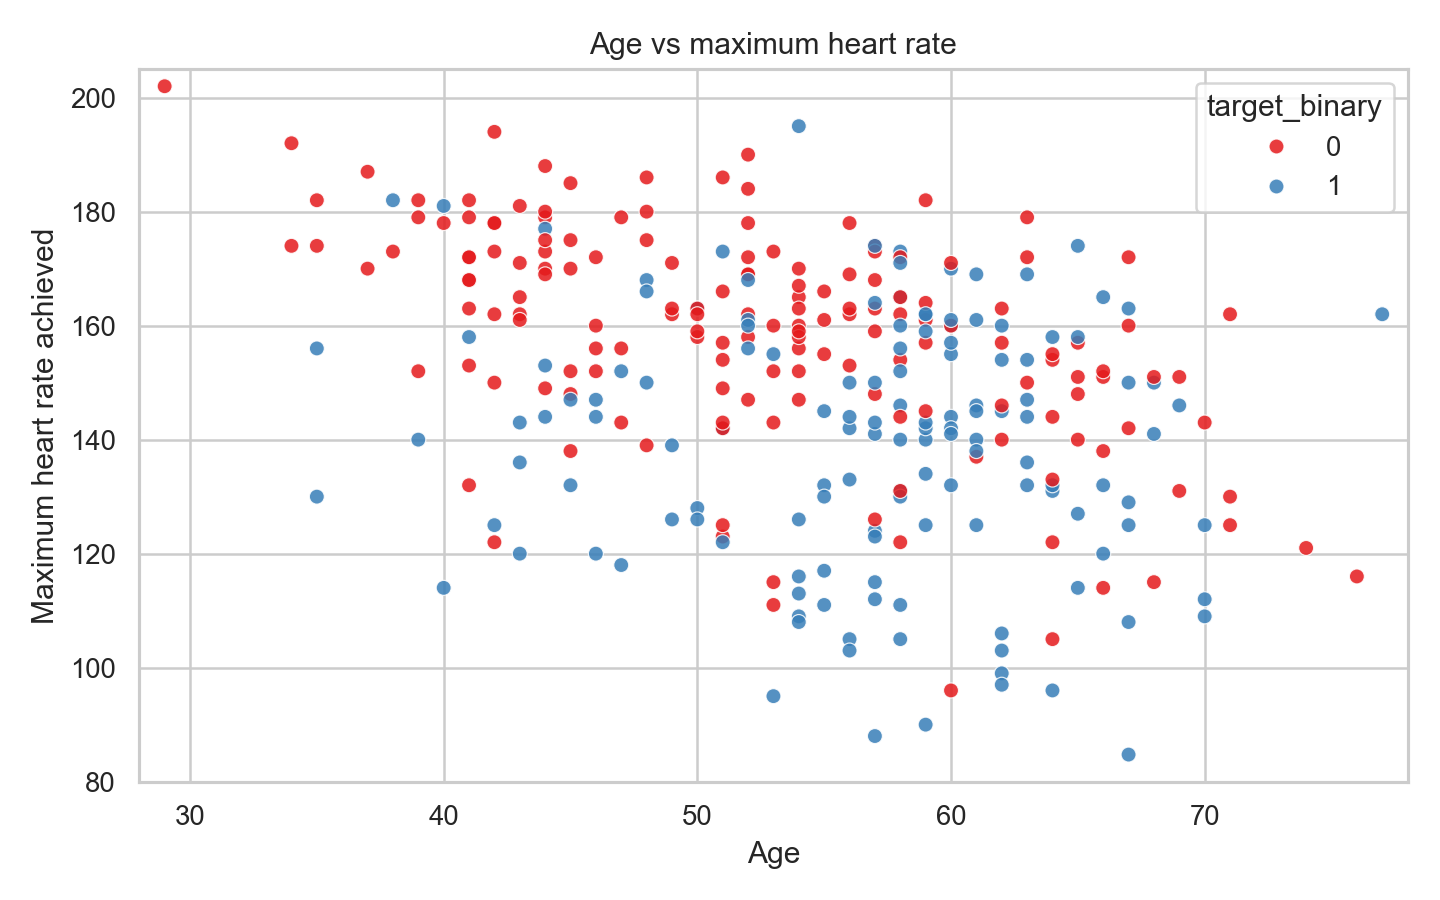
\includegraphics[width=0.90\textwidth]{images/ch1/heart_disease_age_thalach_scatter.png}
\caption[Ví dụ scatter plot trên Heart Disease]{Ví dụ scatter plot age và thalach trên Heart Disease.}
\label{fig:chapter1_scatter_heatmap}
\end{figure}

\begin{figure}[H]
\centering
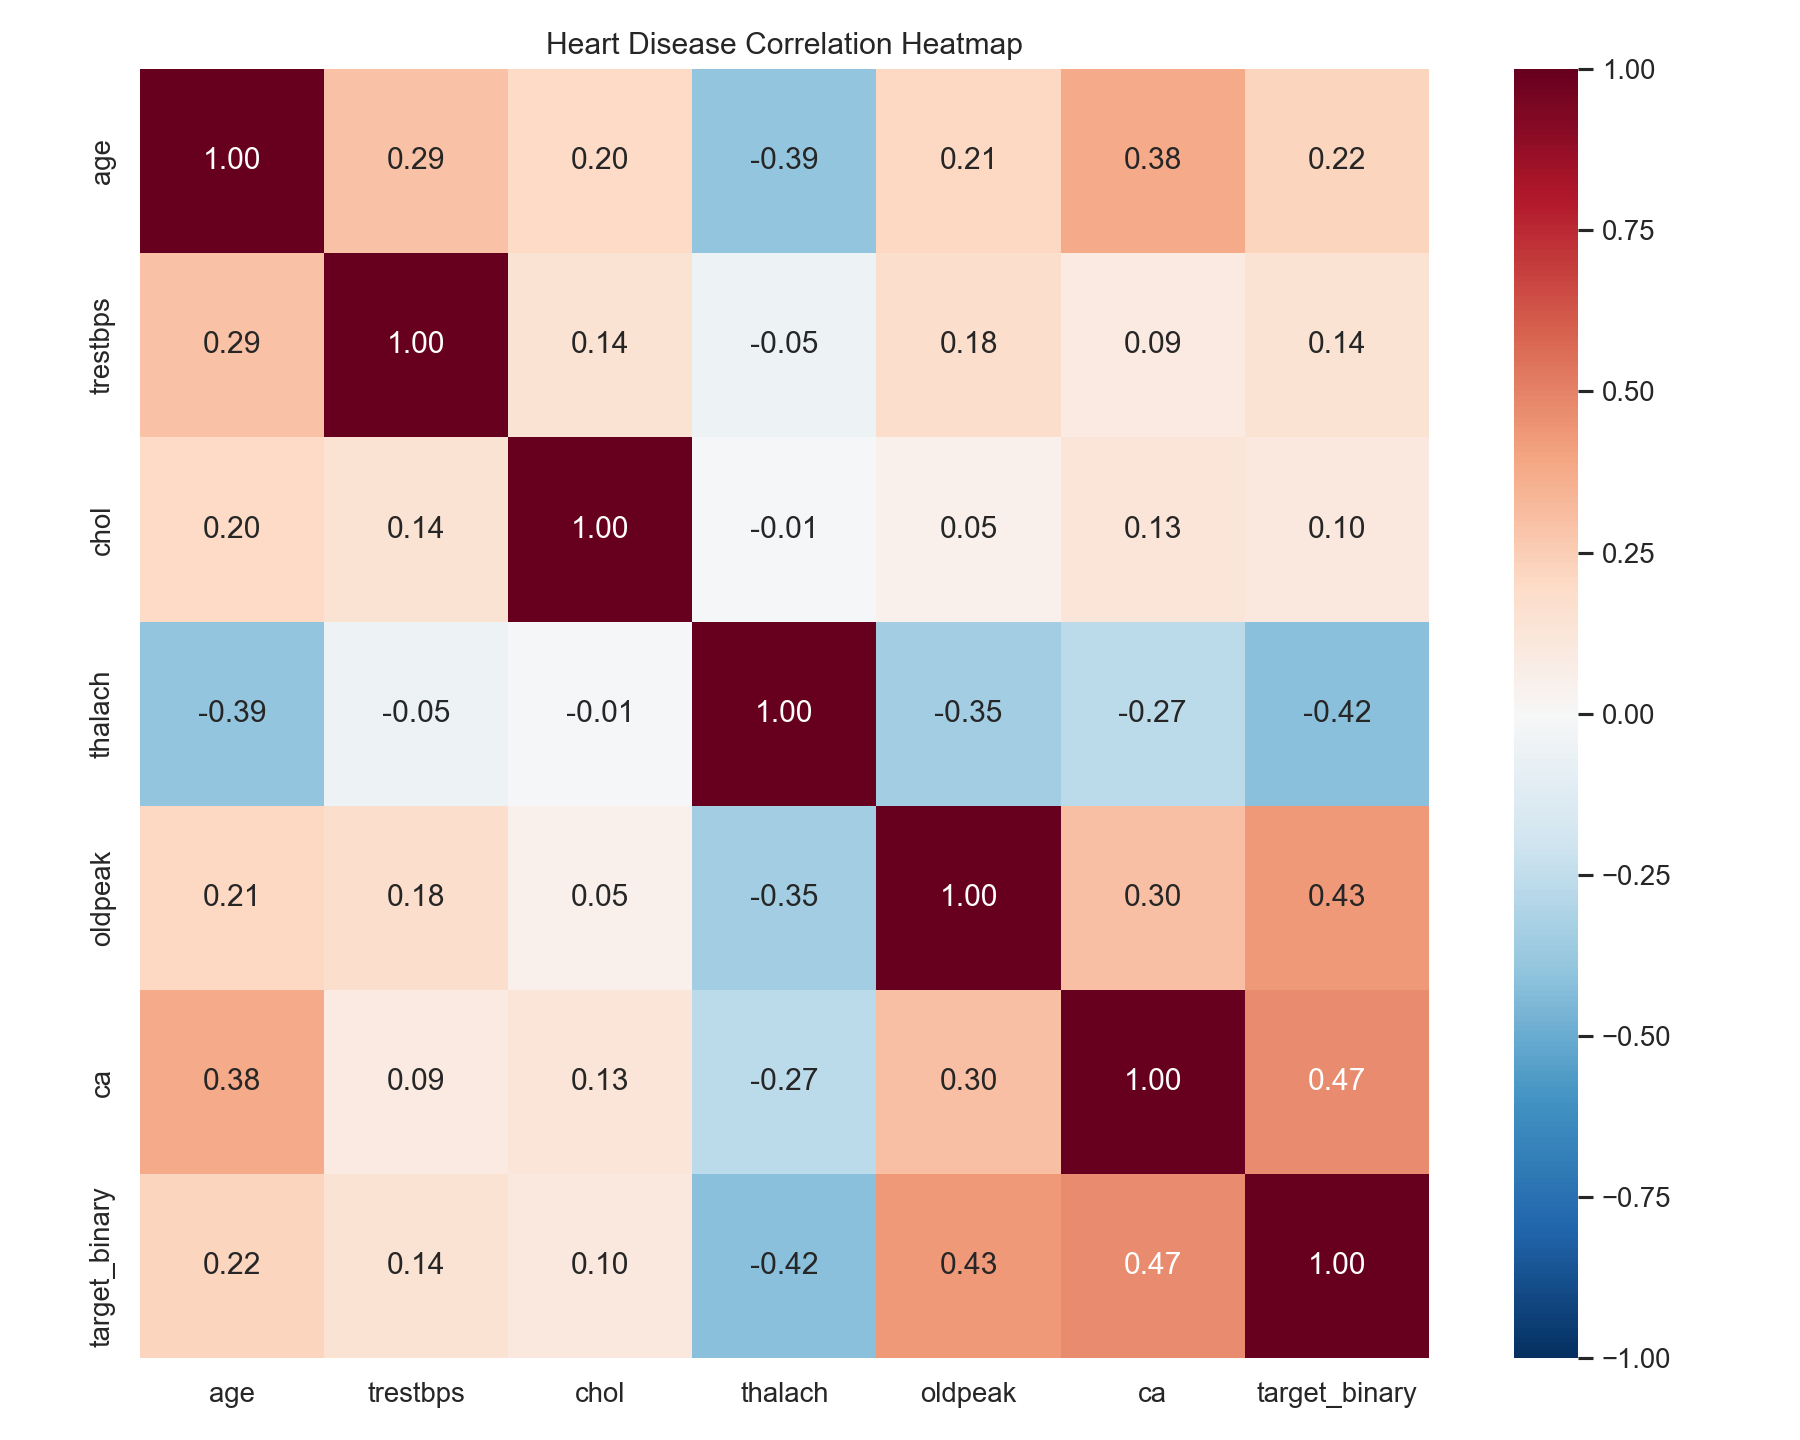
\includegraphics[width=0.95\textwidth]{images/ch1/heart_disease_correlation_heatmap.png}
\caption[Ví dụ correlation heatmap trên Heart Disease]{Ví dụ correlation heatmap trên Heart Disease.}
\label{fig:heart_corr_heatmap}
\end{figure}

\textbf{Lý do chọn biểu đồ.} Scatter plot phù hợp để kiểm tra quan hệ giữa hai biến định lượng \texttt{age} và \texttt{thalach}; heatmap phù hợp để xem nhanh toàn bộ ma trận tương quan.

\textbf{Nhận xét.} Hình \ref{fig:chapter1_scatter_heatmap} minh họa vai trò của trực quan hóa đa biến. Scatter plot cho phép quan sát mối quan hệ giữa tuổi và nhịp tim tối đa, đồng thời tô màu theo nhãn bệnh. Heatmap cho phép nhìn nhanh cặp biến nào có liên hệ tuyến tính mạnh. Trong quy trình phân tích, hai biểu đồ này giúp hình thành giả thuyết trước khi đưa dữ liệu vào mô hình học máy.

\section{Liên kết lý thuyết với các chương sau}

Chương 2 cung cấp ngôn ngữ chung để đọc các kết quả ở Chương 4 và Chương 5. Các chỉ số mean, median, IQR và standard deviation sẽ được dùng để so sánh trước/sau tiền xử lý. Các biểu đồ histogram, boxplot, line chart và heatmap sẽ được dùng để phát hiện đặc trưng dữ liệu. Các nhận xét này tiếp tục làm cơ sở cho lựa chọn mô hình, diễn giải sai số và so sánh với nghiên cứu liên quan.

